\documentclass[final,3p,times,twocolumn,fleqn]{elsarticle}
\usepackage[american]{babel}
\usepackage[font=normal]{caption}
\usepackage[font=normal]{subcaption}
\usepackage[tensorialbold]{userCommands}
\usepackage{empheq}
\usepackage{tikz} % geometrical figures
\usetikzlibrary{calc,trees,positioning,arrows,chains,shapes.geometric,decorations.pathreplacing,decorations.pathmorphing,shapes,
    matrix,shapes.symbols,shapes.multipart,patterns,shapes,snakes,pgfplots.groupplots,spy,backgrounds}
\usetikzlibrary{external}
\tikzexternalize[prefix=external/]
\usetikzlibrary{spy,backgrounds}
\usetikzlibrary{decorations.markings}
\usetikzlibrary{arrows.meta}
\tikzset{
  arrows along my path/.style={
    postaction={
      decorate,
      decoration={
        markings,
        mark=between positions 0.03 and 1 step 24pt with {\arrow{Stealth[length=8pt]}},
   }}}}

\usepackage{pgfplots} % pdf picture declaration

\usepackage{array}
\newcolumntype{M}[1]{>{\centering\arraybackslash}m{#1}}
\newcolumntype{N}{@{}m{0pt}@{}}


%% The amssymb package provides various useful mathematical symbols
\usepackage{amssymb}
\usepackage{lineno}
\usepackage{float}
% \linenumbers

\usepackage{float}


\usepackage{mathtools}
\mathtoolsset{showonlyrefs}

\journal{International Journal of Solids and Structures}

\pgfplotsset{%compat=1.3,
  %compat=1.8,
  compat=newest,
  grid=both,
  tick label style={font=\normalsize},
  label style={font=\normalsize},
  legend style={font=\normalsize},
  legend cell align={left},
  yticklabel style={/pgf/number format/fixed},
  %scaled y ticks=false,
  % define user colormap
  colormap={tol}{[1cm] rgb255(0cm)=(120,28,129) rgb255(1cm)=(63,96,174) rgb255(2cm)=(83,158,182) rgb255(3cm)=(109,179,136) rgb255(4cm)=(202,184,67) rgb255(5cm)=(231,133,50) rgb255(6cm)=(217,33,32)}
}

\definecolor{Purple}{RGB}{120,28,129}
\definecolor{Orange}{RGB}{231,133,50}
\definecolor{Blue}{RGB}{63,96,174}
\definecolor{Red}{RGB}{217,33,32}
\definecolor{Duck}{RGB}{83,158,182}
\definecolor{Green}{RGB}{109,179,136}
\definecolor{Yellow}{RGB}{202,184,67}

\newcommand{\review}[1]{\color{Red}#1\color{black}}

\newtheorem{remark}{Remark}


\begin{document}

\begin{frontmatter}


  %% Title, authors and addresses

  %% use the tnoteref command within \title for footnotes;
  %% use the tnotetext command for theassociated footnote;
  %% use the fnref command within \author or \address for footnotes;
  %% use the fntext command for theassociated footnote;
  %% use the corref command within \author for corresponding author footnotes;
  %% use the cortext command for theassociated footnote;
  %% use the ead command for the email address,
  %% and the form \ead[url] for the home page:
  %% \title{Title\tnoteref{label1}}
  %% \tnotetext[label1]{}
  %% \author{Name\corref{cor1}\fnref{label2}}
  %% \ead{email address}
  %% \ead[url]{home page}
  %% \fntext[label2]{}
  %% \cortext[cor1]{}
  %% \address{Address\fnref{label3}}
  %% \fntext[label3]{}
  
  %\title{Solving hyperbolic problems in hyperelastic-plastic solids with the Discontinuous Galerkin Material Point Method}
  \title{On the characteristic structure of solutions of hyperbolic systems in two-dimensional elastic-plastic solids.}
  
  %% use optional labels to link authors explicitly to addresses:
  %% \author[label1,label2]{}
  %% \address[label1]{}
  %% \address[label2]{}
  
  \author{Adrien Renaud$^1$, Thomas Heuz{\'e}, Laurent Stainier}
  
  \address{$^1$ Research Institute in Civil and Mechanical Engineering (GeM, UMR 6183 CNRS)\\
    Ecole Centrale de Nantes \\
    1 rue de la No\"e, Nantes\\
    e-mail: \{adrien.renaud,thomas.heuze,laurent.stainier\}@ec-nantes.fr}
  
  \begin{abstract}
  \end{abstract}
  
  \begin{keyword}
  \end{keyword}


\end{frontmatter}


%% Faire un historique des formulations faites.
%% Formuler le problème à notre sauce et identifier les cas évoqués en intro en particularisant les modules tangents etc. a ce moment, parler des trajets de chargement et des types d'ondes


\section{Introduction}
\label{sec:introduction}
The numerical simulation of physical problems modeled by means of hyperbolic partial differential equations involves the solution of possibly discontinuous waves.
%
The precise tracking of those waves is of major importance in solid mechanics, especially for history-dependent constitutive equations, as it allows to properly assess the residual states.
\review{More specifically, high-speed forming techniques such that electromagnetic forming \cite{Formage} also requires the tracking of solid interfaces.}   
% \note{(a) Examples of applications that involve large deformations}
% \note{Discontinuities + Large deformations!!}
%
Nevertheless, the accurate simulation of such problems can be prevented by several reasons.
%% Mesh-based Lagrangian
First, Lagrangian formulations of mesh-based approaches such as the widely used Finite Element (FEM) \cite{Belytschko} and Finite Volume (FVM) \cite{Leveque} methods become less accurate for very large deformations due to sever distortions of the mesh.
%% Mesh-based Eulerian and ALE
Although those instabilities can be avoided by resorting to Eulerian or Arbitrary Lagrangian-Eulerian formulations, other difficulties arise owing to additional diffusive projections of fields.
%% Time integration
Second, it is well-known that explicit finite element schemes can exhibit numerical noise near sharp solutions that can be hard to remove with artificial viscosity without loss of accuracy.
Such oscillations can nevertheless be removed from FVM solutions due to numerical fluxes involved in the formulation, allowing the building of Total Variation Diminishing (TVD) schemes \cite{Harten}.
%% DG
The Discontinuous Galerkin approximation in space \cite{NeutronDG}, combined with FEM (DGFEM), enables to take advantage of similar interface fluxes so as to construct Total Variation Diminishing in the Means (TVDM) finite element procedures \cite{Cockburn}.
%% Time integration in DGFEM -> STDG
While the introduction of the DG approximation within FEM schemes enables to avoid non-physical oscillations, providing the use of suitable limiters \cite{vanLeer_Limiters}, these approaches are constrained by a restrictive CFL condition \cite{DGFEM_CFL} and hence, suffer from numerical diffusion.
Space-time DGFEM formulations \cite{ST_DGFEM1} enable to circumvent this drawback but are nonetheless subject to mesh entanglement.
%\review{Moreover, the satisfaction of the compatibility condition between reference and updated configurations, through the Piola identity, is not a straightforward undertaking in Lagrangian formulations \cite{Vilar_PiolaIdentity,LagrangianDG_thesis}, which is also the case for finite volumes \cite{Haider_FVM}.
%In other words, updating the geometry based on discontinuous velocities and deformation gradients across element faces may lead to discontinuities in the displacement vector.}


%% MPM
One possibility to avoid mesh tangling instabilities while providing a material description of the motion is to use mesh-free approaches such as those of the Particle-In-Cell (PIC) family \cite{PIC} and, in particular, the Material Point Method \cite{Sulsky94}.
The MPM is based on a dual discretization of a domain made of a collection of material points lying in an arbitrary grid.
A discrete system is solved on the grid, whereas the loading history is stored at particles during the motion so that field projections, which introduce some freedom into the scheme, are required.
%
Indeed, the updated velocity at the grid level can be directly interpolated to the particles according to the original PIC procedure.
Alternatively, the particle velocities can be updated by interpolating the nodal acceleration resulting from the solution of the discrete system, as introduced in PIC by the FLuid Implicit Particle method (FLIP) \cite{FLIP}.
The latter allows to reduce numerical diffusion at the cost of spurious oscillations \cite{PIC_Nishiguchi}.
Recently, a tunable mapping procedure, based on a parameter $m$ that completely eliminates the noise in MPM solutions, has been proposed in the Extended PIC of order $m$ (XPIC(m)) \cite{XPIC}.
A classical interpolation is selected for $m=1$ whereas the mapping tends to FLIP one as $m\rightarrow \infty$.
Nevertheless, the numerical diffusion still prevents from capturing (discontinuous) waves.

%% DGMPM 
\review{
  %A different point of view, which is followed in the Discontinuous Galerkin Material Point Method (DGMPM) \cite{DGMPM,Thesis}, is that the numerical diffusion exhibited by the PIC can be limited by reducing the domain of influence of nodes rather than modifying the projections themselves.
  Note also that the numerical diffusion exhibited by the PIC can be limited by reducing the domain of influence of nodes rather than modifying the projections themselves.
  This approach is followed in the Discontinuous Galerkin Material Point Method (DGMPM) \cite{DGMPM,Thesis}.
  The introduction of the DG approximation within the MPM, combined with the use of the PIC projection, thus aims at providing non-oscillating discontinuous solutions with low numerical diffusion due to the support of the shape functions that reduces to one cell.
  Therefore, the DGMPM enables to take advantage of space-DGFEM and MPM in order to accurately follow waves in finite-deforming media.
}
%
In that method, the weak form of a system of conservation laws is written on an arbitrary grid and numerical fluxes arising from the DG approximation are computed at cell faces by means of an approximate Riemann solver.
Those intercell fluxes allow to take into account the characteristic structure of hyperbolic problems, and in particular the transverse propagation of waves through the use of the Corner Transport Upwind method (CTU) \cite{Colella_CTU} developed for finite volumes.
The CTU is however reformulated in order to fit the DGMPM approximation, in which fields are edge-wise constant in Riemann problems rather than cell-wise constant as it is the case for FVM.
%% Arbitrary grid
Furthermore, as in MPM, all the fields are stored at material points moving in the arbitrary grid, the mapping between nodes and particles being made with PIC projection so that non-oscillating solutions are provided.
\review{Hence, the geometry is updated at the particles level based on a single-valued velocity field. %, in such a way that the difficulties related to the Piola identity are expected to vanish, though it has not been shown so far.
  %% Total Lagrangian
  As a first development step, the DGMPM has been constructed upon a total Lagrangian formulation.
  %
  The numerical results provided by the method for a plane wave problem in a finite-deforming hyperelastic material showed excellent agreement with the exact solution consisting of either a shock or a rarefaction wave \cite{DGMPM}.
  It is worth noticing that similar results can be obtained with the FVM written in the reference configuration, the key point being however that the update of the geometry is straightforward in the DGMPM.
  %
  Furthermore, an interesting feature of the method consists in allowing the employment of mesh adaption strategies so that waves can be accurately captured in the current configuration.
  On the other hand, only linear shape functions leading to a first-order accuracy \cite{Thesis} have been considered, the extension of the method to higher-order approximations being the object of ongoing works.
  The low-order approximation is however not seen as a shortcoming for now since the development of the method has been focused so far on capturing discontinuous solutions for which the accuracy of any numerical scheme falls to one \cite{Leveque}.
}
%Although the equations of solid mechanics are solved in the reference configuration according to a total Lagrangian formulation, an interesting feature of the method consists in allowing the employment of mesh adaption strategies so that waves can be accurately captured in the current configuration.
%% CFL depending on the space discretization
Nonetheless, the stability of the DGMPM highly depends on the distribution of particles inside the computational grid.
Indeed, the stability analysis of the one-dimensional DGMPM scheme coupled to the forward Euler time integration \cite{DGMPM} yields a stability condition that depends on the space discretization and the CFL number.
%
Conversely, one can ensure the stability for a given distribution of material points by finding the CFL number satisfying the aforementioned relation.
%
Such a condition, which does not exist for the MPM and other DGMPM discretizations, is crucial since it allows to: (i) ensure the stability of the scheme while minimizing the numerical diffusion; (ii) adapt the Courant number when the grid is reconstructed; (iii) adapt the grid so that a given CFL condition is satisfied.
It is the purpose of this paper to provide the stability conditions for the one-dimensional DGMPM scheme combined with the two-stage second-order Runge-Kutta (RK2) time discretization and for the two-dimensional DGMPM coupled to the forward Euler algorithm.
\review{
  Although the solution of linear equations is considered here, the results presented must be put into the context of the problems aimed by the method, involving large deformation, and for which the DGMPM enables plenty of perspectives. 
  }

%% Organization of the paper
In the following, the DGMPM discrete system for the multi-dimensional scalar linear advection equation is derived and the computation of interface fluxes, as well as the solution scheme, are recalled in section \ref{sec:dgmpm}.
In particular, we shall see that the adaptation of the Corner Transport Upwind method (CTU) \cite{Colella_CTU} to DGMPM leads to the same corrections of intercell fluxes as for finite volumes.
Second, the system resulting from the combination of DGMPM and RK2 discretization is specialized to one-dimensional problems in section \ref{sec:1d_stab} so that the von Neumann linear stability analysis is carried out.
At last, the same approach is followed in section \ref{sec:2d_stab} for the DGMPM scheme coupled to the forward Euler time integration applied to the two-dimensional problem.


%%% Local Variables:
%%% mode: latex
%%% TeX-master: "manuscript"
%%% End:



\section{Elastic-plastic wave structure in two space dimensions}
\label{sec:charac_plast}
%% Comment the possibility of widening the approach to kinematic hardening ?
\subsection{Governing equations}
We are concerned with linear isotropic hardening materials which elastic domain is given by the von-Mises yield surface, under isothermal deformations in the linearized geometrical framework.
The balance equation of linear momentum with neglected body forces, and the geometrical balance equations are:  
\begin{equation}
  \label{eq:ch5_balance_equations}
  \left\lbrace \begin{aligned}
    %\label{eq:ch5_linear_momentum}
    & \rho \dot{\vect{v}} - \nablav \cdot \tens{\sigma} = \vect{0} \\
    %\label{eq:ch5_linear_momentum}
    &  \dot{\tens{\eps}} - \nablav \cdot \(\frac{\vect{v}\otimes \tens{I} + \tens{I} \otimes \vect{v}}{2}\) = \vect{0} 
  \end{aligned} \right.
\end{equation}
In addition, the elastic-plastic constitutive equations derived from thermodynamics in section \ref{sec:constitutive-equations} are recalled here:
\begin{subequations}
  \label{eq:ch5_plasticity_equations}
  \begin{empheq}[left=\empheqlbrace]{align}
    \label{eq:ch5_von-Mises_yield}
    & f\(\tens{\sigma},\Acb \)= \sqrt{\frac{3}{2}}\norm{\tens{s}} - \(R(p)+\sigma^y\) \equiv 0,\quad \text{with }\tens{s}=\tens{\sigma}-\frac{1}{3}\tr \tens{\sigma} \tens{I} \\
    % \label{eq:ch5_kin_hard}
    % & \tens{Y}=\frac{2}{3}C\tens{\eps}^p \\
    \label{eq:ch5_iso_hard}
    & R(p)=C \: p \\
    \label{eq:elastoplastic_tangent}
    & \tens{\dot{\sigma}}=\(\Cbb^{elast} - \beta\:\tens{s}\otimes\tens{s} \):\tens{\dot{\eps}} = \Cbb^{ep}:\tens{\dot{\eps}} \\
    \label{eq:ch5_plastic_flow}
    & \beta = \frac{6\mu^2}{3\mu +C}\times\frac{1}{\tens{s}:\tens{s}}\\
    \label{eq:ch5_EP_acoustic}
    & A_{ij}^{ep}=  A_{ij}^{elast} -  \beta (n_k s_{ki})(s_{jl}n_l)
  \end{empheq}
\end{subequations}
In the expression of von-Mises yield function \eqref{eq:ch5_von-Mises_yield}, the (positive) linear isotropic hardening law \eqref{eq:ch5_iso_hard} is considered.
Moreover, the elastoplastic acoustic tensor \eqref{eq:ch5_EP_acoustic} is decomposed as an elastic part $A_{ij}^{elast}$ and a plastic part depending on the direction of the plastic flow through the coefficient $\beta$ \eqref{eq:ch5_plastic_flow}.
%At last, the (isotropic)elasticity tensor $\Cbb$ in equation \eqref{eq:elastoplastic_tangent} can be inverted to yield the following elastic law:
By inverting the (isotropic)elasticity tensor $\Cbb$ involved in equation \eqref{eq:elastoplastic_tangent}, the following elastic law is written in the isotropic case:
\begin{equation}
  \label{eq:ch5_elastic_inverse}
  \tens{\eps}^e = \frac{1+\nu}{E} \tens{\sigma} - \frac{\nu}{E} \tr \tens{\sigma} \tens{I}
\end{equation}
with Young's modulus $E$ and Poisson's ration $\nu$.

The quasi-linear form of the sets of equations \eqref{eq:ch5_balance_equations} and \eqref{eq:ch5_plasticity_equations} in a Cartesian coordinates system and an arbitrary direction $\vect{n}$ is:
\begin{equation}
  \label{eq:ch5_quasilinear_normal}
  \Qcb_t + \Jbsf \drond{\Qcb}{x_n} = \vect{0} 
\end{equation}
where $x_n=\vect{x}\cdot\vect{n}$, $\Qcb=\matrice{\vect{v}\\ \tens{\sigma}}$, and $\Jbsf$ is the Jacobian matrix.
It has been shown in section \ref{sec:characteristic_analysis} that the $3$ eigenvalues $\omega^p$ and eigenvectors $\vect{l}^p$ of the acoustic tensor lead to $6$ left characteristic fields of the Jacobian matrix $\{c_K;\Lcb^K\}$ according to:
\begin{equation}
  \label{eq:ch5_left_eigenfields}
  \left\lbrace \pm \sqrt{\frac{\omega_p}{\rho}} ; \quad \[\: \pm \rho\sqrt{\frac{\omega_p}{\rho}} \vect{l}^p , -\vect{l}^p\otimes \vect{n} \:\]  \right\rbrace ,\quad p=1,2,3
\end{equation}
In addition, three independent left eigenvectors associated to the zero eigenvalue of system \eqref{eq:ch5_quasilinear_normal}, which is of multiplicity $3$, are found by solving:
\begin{equation}
  \label{eq:ch5_null_eigen}
  \tens{\sigma}^K:\(\Cbb^{ep}\cdot  \vect{n}\) =\vect{0},\quad K=1,2,3
\end{equation}

The present formulation differs from those of \textsc{Bleich} \cite{Bleich}, \textsc{Clifton} \cite{Clifton}, and hence these of \textsc{Ting} and \textsc{Nan} \cite{Ting68} and \textsc{Ting} \cite{Ting69}, in that equation  \eqref{eq:ch5_quasilinear_normal} is based on the elastoplastic stiffnesses rather than softenesses.
As a consequence, it will be seen in what follows that the equations can be easily specialized to plane strain and plane stress cases.
%In what follows, the above equations are specified to plane strain and plane stress cases.
\subsection{Problems in two space dimensions}
We now focus on the solid domain $x_1 \times x_2 \times x_3 \in [0,\infty[ \times [-h,h] \times [-e,e]$ in a Cartesian coordinates system, where $e$ and $h$ are arbitrary lengths.
%The solid is subject in the plane $x_1=0$ to a traction force $\vect{T}^1$ restricted to the $(\vect{e}_1,\vect{e}_2)$ plane, that is $T_3=0$.
It is assumed that all quantities depend solely on $x_1$ and $x_2$ except the velocity component $v_3$ that may depend on $x_3$.
In particular, it is the case for $e \ll h$.

The solid is under plane strain conditions, that is $\tens{\eps}\cdot\vect{e}_3=\vect{0}$, if the velocity $\vect{v}$ does not depend on $x_3$ and if $v_3$ vanishes.
Thus, combining the additive partition of the infinitesimal strain tensor: $\tens{\eps}=\tens{\eps}^e+\tens{\eps}^p$, with the elastic law \eqref{eq:ch5_elastic_inverse} and the kinematic condition $\eps_{33}=0$, one gets:
\begin{equation}
  \label{eq:plane_strain_stress33}
  \sigma_{33}=\nu\(\sigma_{11}+\sigma_{22}\) - E\eps^p_{33}
\end{equation}
Hence, the quasi-linear form \eqref{eq:ch5_quasilinear_normal} reduces for plane strain problems to a system of dimension $5$ with unknowns $v_1,v_2, \sigma_{11},\sigma_{12}$, and $\sigma_{22}$.


Alternatively, a plane stress state ($\tens{\sigma}\cdot\vect{e}_3=\vect{0}$) is assumed if the planes $x_3=\pm h$ are traction free and $e\ll h$.
As a result, the stress component $\sigma_{33}$ can be removed from the system \eqref{eq:ch5_quasilinear_normal}.
Nevertheless, the tangent modulus must account for the vanishing out-of-plane stress component.
Specialization of equation \eqref{eq:elastoplastic_tangent} to $\sigma_{33}$ yields:
\begin{equation*}
  \dot{\sigma}_{33}=C^{ep}_{33ij} \dot{\eps}_{ij} =0
\end{equation*}
from which one writes:
\begin{equation*}
  C^{ep}_{3333} \dot{\eps}_{33} = - C^{ep}_{33ij}\dot{\eps}_{ij} \quad i,j=\{1,2\}
\end{equation*}
Hence, the constitutive equations are rewritten by means of a two-dimensional tangent modulus $\widetilde{\Cbb}^{ep}$:
\begin{equation}
  \label{eq:CP_constitutive}
  \dot{\sigma}_{ij}=C^{ep}_{ijkl} \dot{\eps}_{kl} - \frac{C^{ep}_{ij33}C^{ep}_{33kl}}{C^{ep}_{3333}}\dot{\eps}_{kl}= \widetilde{C}^{ep}_{ijkl} \dot{\eps}_{kl}\qquad i,j,k,l=\{1,2\} 
\end{equation}
The characteristic structure of the problem is then given by this of the associated acoustic tensor $\tens{\widetilde{A}}^{ep}=\vect{n}\cdot\widetilde{\Cbb}^{ep}\cdot \vect{n}$.

The removal of $\sigma_{33}$ from system \eqref{eq:ch5_quasilinear_normal} for both plane strains and plane stresses allows to solve the problem in a two-dimensional setting.
Then, generically denoting the acoustic tensor by $\tens{A}$, the characteristic structures are given by the eigenvalues:
\begin{subequations}
  \begin{alignat}{1}
    \label{eq:ch5_eigenAcc1}
    &\omega_1 = \frac{1}{2}\(A_{11}+A_{22} + \sqrt{(A_{11}-A_{22})^2+{4A_{12}}^2}\) \\
    \label{eq:ch5_eigenAcc2}
    &\omega_2 = \frac{1}{2}\(A_{11}+A_{22} - \sqrt{(A_{11}-A_{22})^2+{4A_{12}}^2}\)     
  \end{alignat}
\end{subequations}
and the associated eigenvectors:
\begin{equation}
  \label{eq:ch5_eigenvectAcc}
   \vect{l}^1=[ A_{22}-  \omega_1 \:,\: -A_{12}] \qquad ;\qquad  \vect{l}^2=[ -A_{12} \:,\:A_{11}- \omega_2 ]
\end{equation}
From equation \eqref{eq:ch5_left_eigenfields}, we see that two families of waves with celerities $c_f=\pm \sqrt{\omega_1/\rho}$ and $c_s = \pm \sqrt{\omega_2/\rho}$ may travel in the domain.
Those waves are respectively referred to as fast and slow waves.
Note that subtracting equations \eqref{eq:ch5_eigenAcc1} and \eqref{eq:ch5_eigenAcc2} leads to:
\begin{equation}
  \label{eq:diff_celerities}
  \rho c_f^2 - \rho c_s^2 = \sqrt{(A_{11}-A_{22})^2+{4A_{12}}^2} \geq 0
\end{equation}
Hence, the characteristic speed associated to fast waves is always greater than of equal to that of slow waves.

The four left eigenfields of the Jacobian matrix thus read:
\begin{subequations}
  \begin{alignat}{1}
    \label{eq:ch5_Jac_eigenfield_fast}
    &\left\lbrace \pm c_f ; \quad \Lcb^{c_f^\pm}=\[\: \pm \rho c_f \vect{l}^1 , -\vect{l}^1\otimes \vect{n} \:\]  \right\rbrace \\
  \label{eq:ch5_Jac_eigenfield_slow}
    &\left\lbrace \pm c_s ; \quad \Lcb^{c_s^\pm}=\[\: \pm \rho c_s \vect{l}^2 , -\vect{l}^2\otimes \vect{n} \:\]  \right\rbrace
  \end{alignat}
\end{subequations}
where $\Lcb^{c_f^+}$ and $\Lcb^{c_f^-}$ are associated to the right-going and left-going fast waves respectively.
The same goes for $\Lcb^{c_s^+}$ and $\Lcb^{c_s^-}$.
Furthermore, one stationary wave associated to the zero eigenvalue of the Jacobian matrix, and which left eigenvector satisfies equation \eqref{eq:ch5_null_eigen}, has to be added:
\begin{equation}
  \label{eq:ch5_null_left_eigen}
  {\Lcb^0}^T = \matrice{v_1^0 \\[5.pt] v_2^0 \\[5.pt] \sigma_{11}^0 \\[5.pt] \sigma^0_{22} \\[5.pt] \sigma^0_{12} }= \matrice{0 \\[5.pt] 0 \\[5.pt] \(C_{121i}C_{222j}-C_{221i}C_{122j}\)n_in_j \\[5.pt] \(C_{111i}C_{122j}-C_{112i}C_{121j}\)n_in_j \\[5.pt] \(C_{112i}C_{221j}-C_{111i}C_{222j}\)\frac{n_in_j}{2}} = \matrice{0 \\ 0 \\ \alpha_{11} \\ \alpha_{22} \\ \alpha_{12} }
\end{equation}
with $\Cbb=\Cbb^{ep}$ for plain strain and $\Cbb=\widetilde{\Cbb}^{ep}$ for plane stress.
%In particular, $\Cbb$ reduces to the elastic stiffness tensor when no plastic flow occurs so that the characteristic structure involves the speeds of elastic pressure waves $c_1$ and shear waves $c_2$. 

It has been seen in section \ref{sec:SVK_solution} that the solution of non-linear problems may contain shock and/or simple waves.
Nevertheless, we restrict here to simple waves by assuming that: (i) the characteristic speeds satisfy $c_1 \geq c_f \geq c_2 \geq c_s $, where $c_1$ and $c_2$ are the speeds of elastic pressure and shear discontinuities respectively; (ii) $c_f$ and $c_s$ monotonically decrease with the hardening of the material; (ii) the computational domain is in an initial natural, plastic strain free state.

The characteristic equations $\Lcb^K \cdot d\Qcb = 0$ are then written:
\begin{subequations}
  %\label{eq:ch5_ODEs}
  \begin{alignat}{3}
    \label{eq:charac_fr}
    & \rho c_f \vect{l}^1 \cdot d\vect{v} - l^1_i n_j d\sigma_{ij} =0 \qquad && \text{along }\: dx/dt = c_f\\
    \label{eq:charac_fl}
    -& \rho c_f \vect{l}^1 \cdot d\vect{v} - l^1_i n_j d\sigma_{ij} =0 \qquad && \text{along }\: dx/dt = - c_f \\
    \label{eq:charac_sr}
    & \rho c_s \vect{l}^2 \cdot d\vect{v} - l^2_i n_j d\sigma_{ij} =0 \qquad  && \text{along }\: dx/dt =  c_s \\
    \label{eq:charac_sl}
    -& \rho c_s \vect{l}^2 \cdot d\vect{v} - l^2_i n_j d\sigma_{ij} =0 \qquad  && \text{along }\: dx/dt = - c_s \\
    \label{eq:charac_contact}
    &\alpha_{11}d\sigma_{11} + \alpha_{12}d\sigma_{12} + \alpha_{22}d\sigma_{22}=0 \qquad && \text{along }\: dx/dt =0 
  \end{alignat}
\end{subequations}
Integration of equations \eqref{eq:charac_fr} to \eqref{eq:charac_contact} leads to integral curves through simple waves in which several stress components vary, hence the name of combined-stress simple waves \cite{CRISTESCU19591605}.
Following \cite{Clifton}, the method of characteristic is applied by combining equations \eqref{eq:charac_fr} to \eqref{eq:charac_contact}.
\begin{figure}[h!]
  \centering
  \subcaptionbox{Slow simple wave \label{subfig:slowWave}}{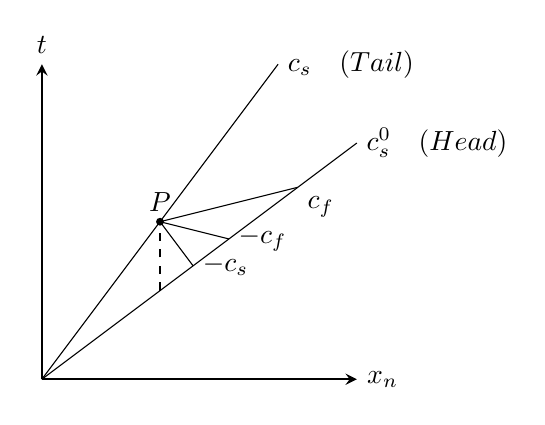
\begin{tikzpicture}[scale=1.,>=stealth] 
  \newcommand\shift{5.}
  %% Slow
  \draw[thick,->] (0,0) -- (4.,0) node[right] {$x_n$};
  \draw[thick,->] (0,0) -- (0.,4) node[above] {$t$};
  % Slope = 0.75
  \draw (0,0) -- (4,3.) node [right] {$c_s^0 \quad (Head)$};
  % Slope = 4./3.
  \draw (0,0) -- (3.,4.) node [right] {$c_s \quad (Tail)$};

  \fill[black] (1.5,1.5*4./3.) circle (0.05) node [above] {$P$};
  %% Other characteristics
  % stationary
  \draw[dashed] (1.5,0.75*1.5) -- (1.5,1.5*4./3.);
  % fast plus (slope =+-0.25)
  \newcommand\px{1.5}
  \newcommand\py{1.5*4./3.}
  \draw (2.*\py-0.5*\px,1.5*\py-3.*\px/8.) node [below right] {$c_f$}-- (1.5,1.5*4./3.) ;
  % fast minus
  \draw (\py+0.25*\px,0.75*\py+3.*\px/16.) node [right] {$-c_f$} -- (1.5,1.5*4./3.) ;
  % slow minus (slope=-4./3.)
  \draw (12.*\py/25.+16.*\px/25.,9.*\py/25.+36.*\px/75.) node [right] {$-c_s$} -- (1.5,1.5*4./3.) ;
\end{tikzpicture}


%%% Local Variables:
%%% mode: latex
%%% TeX-master: "../../mainManuscript"
%%% End:
} \qquad
  \subcaptionbox{Fast simple wave \label{subfig:fastWave}}{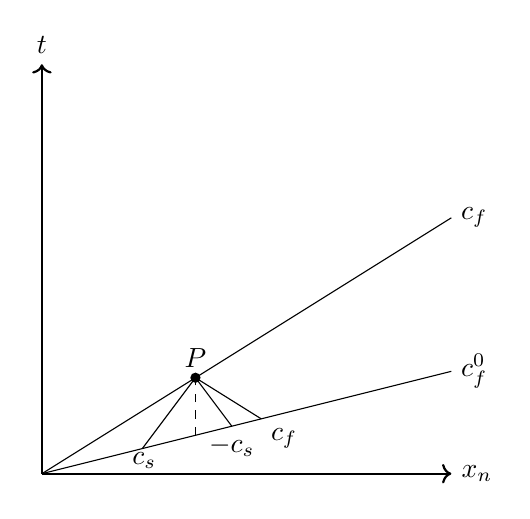
\begin{tikzpicture}[scale=1.3] 
  \newcommand\shift{5.}
  %% Fast
  \draw[thick,->] (0+\shift,0) -- (4.+\shift,0) node[right] {$x_n$};
  \draw[thick,->] (0+\shift,0) -- (0.+\shift,4) node[above] {$t$};
  % Slope = 0.25
  \draw (0+\shift,0) -- (4+\shift,1.) node [right] {$c_f^0$};
  % Slope = 5./8.
  \draw (0+\shift,0) -- (4+\shift,2.5) node [right] {$c_f$};
  
  \fill[black] (1.5+\shift,1.5*5./8.) circle (0.05) node [above] {$P$};
  %% Other characteristics
  \newcommand\pxx{1.5}
  \newcommand\pyy{1.5*5./8.}
  % stationary
  \draw[dashed] (1.5+\shift,1.5/4.) -- (\pxx+\shift,\pyy);
  % fast minus
  \draw (8.*\pyy/7.+5.*\pxx/7.+\shift,2.*\pyy/7.+10.*\pxx/56.) node [below right] {$c_f$}-- (\pxx+\shift,\pyy);
  % slow plus
  \draw (-12.0*\pyy/13.+16.*\pxx/13.+\shift,-3.*\pyy/13.+4.*\pxx/13.) -- (\pxx+\shift,\pyy);
  \node at (-12.0*\pyy/13.+16.*\pxx/13.+\shift+0.02,-3.*\pyy/13.+4.*\pxx/13.-0.12) {$c_s$};
  % slow minus
  \draw (12.0*\pyy/19.+16.*\pxx/19.+\shift,3.*\pyy/19.+4.*\pxx/19.)node [below] {$-c_s$} -- (\pxx+\shift,\pyy);
\end{tikzpicture}


%%% Local Variables:
%%% mode: latex
%%% TeX-master: "../../mainManuscript"
%%% End:
}
  \caption{The method of characteristics through slow and fast simple waves in the $(x_n,t)$ plane.}
  \label{fig:ch5_charac_method}
\end{figure}
The approach consists in tracing every characteristics from some downstream point of a wave where the state vector $\Qcb$ is known, to an upstream point where the solution is seeked. Figures \ref{fig:ch5_charac_method}\subref{subfig:slowWave} and \ref{fig:ch5_charac_method}\subref{subfig:fastWave} schematically illustrate the method for slow and fast simple waves in which the state is known along the head wave and is looked for at point $P$ lying on the tail wave. 
The integral curves through slow and fast simple waves are derived in the next section.

\subsection{Integral curves through simple waves}
The right-going slow waves are first looked at by adding equations \eqref{eq:charac_fr} and \eqref{eq:charac_fl}:
\begin{equation}
  l_i^1 n_j d\sigma_{ij}=0
\end{equation}
Given the geometry of the problem, the vector $\vect{n}$ may be reduced to $\vect{e}_1$ or $\vect{e}_2$.
It therefore comes out:
%In particular, for a vector $\vect{n}$ that is restricted to the axis of the $(\vect{e}_1,\vect{e}_2)$ plane, one gets:
\begin{subequations}
  \begin{alignat}{2}
    \label{eq:sigSlow_n=e1}
    & d\sigma_{11} = - \frac{l^1_2}{l_1^1} d\sigma_{12} = \psi^s_{1}d\sigma_{12} && \qquad \text{for } \:\vect{n}=\vect{e}_1 \\
    \label{eq:sigSlow_n=e2}
    & d\sigma_{22}=- \frac{l_1^1}{l_2^1}  d\sigma_{12} = \psi^s_{2}d\sigma_{12} && \qquad \text{for } \:\vect{n}=\vect{e}_2
  \end{alignat}
\end{subequations}
where $\psi^s_1$ and $\psi^s_2$ are functions of all components of $\tens{\sigma}$. 
Moreover, the $s$ and $f$ superscripts stand for slow and fast waves respectively in the remainder of the manuscript.
With the above equations, the characteristic equation related to the contact wave \eqref{eq:charac_contact} reads:
%Next, the characteristic equation related to the contact wave \eqref{eq:charac_contact} yields:
\begin{subequations}
  \begin{alignat}{2}
    \label{eq:sigContact_n=e1}
    & d\sigma_{22} = -\frac{\psi^s_{1}\alpha_{11}+\alpha_{12}}{\alpha_{22}}d\sigma_{12} && \qquad \text{for } \:\vect{n}=\vect{e}_1 \\
    \label{eq:sigContact_n=e2}
    & d\sigma_{11}= -\frac{\psi^s_{2}\alpha_{22}+\alpha_{12}}{\alpha_{11}} d\sigma_{12} && \qquad \text{for } \:\vect{n}=\vect{e}_2
  \end{alignat}
\end{subequations}
The sets of equations \eqref{eq:sigSlow_n=e1}-\eqref{eq:sigContact_n=e1} and \eqref{eq:sigSlow_n=e2}-\eqref{eq:sigContact_n=e2} show the combined-stress nature of slow simple waves.
% Hence, one stress component may be used as a driving parameter for the two others, as it is the case for $\sigma_{12}$ in equations \eqref{eq:sigSlow_n=e1}, \eqref{eq:sigSlow_n=e2}, \eqref{eq:sigContact_n=e1} and \eqref{eq:sigContact_n=e2}.
On the other hand, the subtraction of equations \eqref{eq:charac_fr} and \eqref{eq:charac_fl} leads to:
\begin{equation*}
  dv_1 = \psi^s_{1}dv_2 = \frac{1}{\psi^s_2}dv_2
\end{equation*}
which, once combined with equations \eqref{eq:sigSlow_n=e1}-\eqref{eq:sigSlow_n=e2} and introduced in \eqref{eq:charac_sl}, yields after simplifications:
\begin{subequations}
  \begin{alignat}{2}
    \label{eq:vSlow_n=e1}
    & dv_1 = -\frac{d\sigma_{11}}{\rho c_s^2} \quad ;\quad  dv_2 = -\frac{d\sigma_{12}}{\rho c_s^2} \qquad & \text{for } \vect{n}=\vect{e}_1\\
    \label{eq:vSlow_n=e2}
    & dv_1 = -\frac{d\sigma_{12}}{\rho c_s^2} \quad ;\quad  dv_2 = -\frac{d\sigma_{22}}{\rho c_s^2} \qquad & \text{for } \vect{n}=\vect{e}_2
  \end{alignat}
\end{subequations}

\begin{remark}
  The integral curves through a left-going slow wave result from the combination of equations \eqref{eq:sigSlow_n=e1}-\eqref{eq:sigSlow_n=e2} introduced in \eqref{eq:charac_sr} rather than \eqref{eq:charac_sl}.
  Therefore, the only difference lies in the signs in equations \eqref{eq:vSlow_n=e1} and \eqref{eq:vSlow_n=e2}
\end{remark}

Similar results are obtained for right-going fast simple waves by using $\vect{l}^2$ instead of $\vect{l}^1$ and $c_f$ rather than $c_s$.
%However, the integral curves involve $\vect{l}^2$ and $c_f$ instead of $\vect{l}^1$ and $c_s$. 
Hence, the evolution in slow and fast waves is governed by the \textit{loading functions}:
\begin{equation}
  \label{eq:loading_func}
  \psi^s_{1}=- \left.\frac{l^1_2}{l_1^1}\right\rvert_{\vect{n}=\vect{e}_1}\quad ,\quad  \psi^s_{2}=- \left.\frac{l_1^1}{l_2^1}\right\rvert_{\vect{n}=\vect{e}_2} \quad ,\quad \psi^f_1=-\left.\frac{l_2^2}{l_1^2}\right\rvert_{\vect{n}=\vect{e}_1} \quad ,\quad \psi^f_2=-\left.\frac{l_1^2}{l_2^2}\right\rvert_{\vect{n}=\vect{e}_2}
\end{equation}
The equations satisfied across right-going slow and fast simple waves are summarized in table \ref{tab:simpleWavesEquations}.
\begin{table}[h!]
  \centering
  \begin{tabular}{cc|ccN}
    \hline
    \multicolumn{2}{c}{Right-going slow wave} \vline& \multicolumn{2}{c}{Right-going fast wave} & \\
    $\vect{n}=\vect{e}_1$ & $\vect{n}=\vect{e}_2$ & $\vect{n}=\vect{e}_1$ & $\vect{n}=\vect{e}_2$&\\
    \hline
    \hline
    $dv_1 = -\frac{d\sigma_{11}}{\rho c_s^2}$ &  $dv_1 = -\frac{d\sigma_{12}}{\rho c_s^2}$ &$dv_1 = -\frac{d\sigma_{11}}{\rho c_f^2}$ &  $dv_1 = -\frac{d\sigma_{12}}{\rho c_f^2}$ &\\ [8pt]
    $dv_2 = -\frac{d\sigma_{12}}{\rho c_s^2}$ & $dv_2 = -\frac{d\sigma_{22}}{\rho c_s^2}$ & $dv_2 = -\frac{d\sigma_{12}}{\rho c_f^2}$ & $dv_2 = -\frac{d\sigma_{22}}{\rho c_f^2}$& \\ [8pt]
    $d\sigma_{11} = \psi^s_{1}d\sigma_{12}$&$d\sigma_{11}= -\frac{\psi^s_{2}\alpha_{22}+\alpha_{12}}{\alpha_{11}} d\sigma_{12}$ &  $d\sigma_{11} = \psi^f_{1}d\sigma_{12}$&$d\sigma_{11}= -\frac{\psi^f_{2}\alpha_{22}+\alpha_{12}}{\alpha_{11}} d\sigma_{12}$ & \\[8pt]
    $d\sigma_{22} = -\frac{\psi^s_{1}\alpha_{11}+\alpha_{12}}{\alpha_{22}}d\sigma_{12}$ & $d\sigma_{22}= \psi^s_{2}d\sigma_{12}$ & $d\sigma_{22} = -\frac{\psi^f_{1}\alpha_{11}+\alpha_{12}}{\alpha_{22}}d\sigma_{12}$ & $d\sigma_{22}= \psi^f_{2}d\sigma_{12}$ & \\[8pt]
    % & & \\
    % & & \\    
    \hline
\end{tabular}
%%% Local Variables:
%%% mode: latex
%%% TeX-master: "../manuscript"
%%% End:

  \caption{Summary of the ODEs satisfied inside right-going slow and fast simple waves.}
  \label{tab:simpleWavesEquations}
\end{table}

The integration of equations gathered in table \ref{tab:simpleWavesEquations} should provide the complete solution of a given problem by means of integral curves or loading paths.
For instance, the velocity resulting from the passage of right-going waves in the direction $\vect{e}_1$ obeys:
\begin{equation}
  \label{eq:integral_example}
  v_1 = v_1^0 - \int_{\tens{\sigma}^0}^{\tens{\sigma}} \frac{d \sigma_{11}}{\rho c^2} \quad ;\quad v_2 = v_2^0 - \int_{\tens{\sigma}^0}^{\tens{\sigma}} \frac{d \sigma_{12}}{\rho c^2}
\end{equation}
where the zero superscript denotes the downstream state.
Nevertheless, \textsc{Clifton} \cite{Clifton} emphasized that depending on the loading conditions, only one simple waves or both may arise in the solution.
Therefore, it is crucial to identify the stress path followed to properly compute integrals \eqref{eq:integral_example}.
%It is thus important to qualify the stress paths through fast and slow waves in order to properly define the upper bound of the integrals of the form \eqref{eq:integral_example}.
This is the purpose of the next section.



%%% Local Variables:
%%% mode: latex
%%% TeX-master: "../mainManuscript"
%%% End:


\section{Loading paths through simple waves}
\label{sec:stress_paths}
It has been highlighted that the complete solution of a hyperbolic system in elastic-plastic solids requires to know \textit{a priori} the wave structure.
The object of this section is to study the mathematical properties of the loading functions \eqref{eq:loading_func} in order to get some clues about the stress paths.
It is believed that the information thus earned could be used to accurately approximate the integration of equations \eqref{eq:integral_example}.
First, general properties holding regardless of the loading conditions are highlighted.
Next, the equations are specialized to plane stress and plane strain cases.

\subsection{The general case}
To begin with, let us look at the product of the two loading functions in a direction of space.
Given the left eigenvectors of the acoustic tensor in equation \eqref{eq:eigenvectAcc}, one has for instance:
%Indeed, considering the left eigenvectors of the acoustic tensor given in equation \eqref{eq:eigenvectAcc}, the product $\psi^s_1\psi^f_1$ reads:
\begin{equation*}
  \psi^s_1\psi^f_1 = \frac{l^1_2}{l^1_1}\: \frac{l_2^2}{l^2_1}  
\end{equation*}
Since the eigenvectors of symmetric second-order tensors all satisfy $\vect{l}^1 \cdot \vect{l}^2=0$, it comes out that the above product is equal to $-1$.
Hence, the loading paths resulting from the integration of the ODEs involving $\psi^s_1$ and $\psi^f_1$ are perpendicular in the stress space.
The same goes for $\psi^s_2 $ and $\psi^f_2 $.
Although this orthogonality has already been noticed for particular plane strain and plane stress cases \cite{Clifton,Ting68}, \emph{the generic formulation proposed here shows that this is valid for all problems in two space dimensions}. 
As a result, the study can be restricted to one function in each direction, say $\psi_1^s$ and $\psi_2^s$.


Second, if the function $\psi_1^s$ vanishes at some point of the stress space, the projection in the $(\sigma_{11},\sigma_{12})$ plane of the loading path followed within a slow wave is vertical according to the ODE \eqref{eq:sigSlow_n=e1} (\textit{i.e} $d\sigma_{11}=0$).
Conversely, if $\psi_1^s\rightarrow \infty$, the loading path is horizontal in the $(\sigma_{11},\sigma_{12})$ plane (\textit{i.e} $d\sigma_{12}=0$).
%Looking for vanishing $\psi^f_1$ or $1/\psi^f_1$ amounts to finding roots of the components of $\vect{l}^2$:
These situations respectively correspond to:
\begin{align}
  \label{eq:first_root}
  \psi_1^s = 0  & \Leftrightarrow A_{12} =0  \\
  \label{eq:second_root}
  \psi_1^s \rightarrow \infty & \Leftrightarrow A_{22} -\omega_1 =0
\end{align}
In particular, if $A_{12}=0$ the denominator of $\psi_1^s$ reads:
\begin{equation}
  A_{22} -\omega_1 = \frac{1}{2}\(A_{22} -A_{11} -\sqrt{(A_{11} -A_{22} )^2 + 4A_{12}^2 }\) = \frac{1}{2}\(A_{22} -A_{11} -\abs{A_{11} -A_{22}}\vphantom{\sqrt{(A_{11} -A_{22} )^2 + 4A_{12}^2 }}\) = -\left\langle A _{11}-A _{22}  \right\rangle
\end{equation}
where $\left\langle \bullet \right\rangle=\frac{1}{2}\(\bullet + \abs{\bullet}\)$ denotes the positive part operator.
Therefore, if $A_{12} =0$ and $A_{11} \neq A_{22} $, one has $\psi^s_1 =0$ and hence $\psi^f_1 \rightarrow -\infty $ by orthogonality.
If moreover $A_{11}  = A_{22} $, both components of the eigenvectors vanish and the functions $\psi^s_1$ and $\psi^f_1$ are undetermined.
Note also that in this case, the characteristic speeds of simple waves are identical according to  equations \eqref{eq:eigenAcc1} and \eqref{eq:eigenAcc2}.
  % \begin{equation}
  %   \label{eq:diff_celerities}
  %   \rho c_f^2 - \rho c_s^2 = \sqrt{(A_{11}-A_{22})^2+{4A_{12}}^2} 
  % \end{equation}
  % Then, it follows that the simultaneous satisfaction of conditions \eqref{eq:first_root} and \eqref{eq:second_root} leads to
As a result, the situation $c_f=c_s$ corresponds to a loss of hyperbolicity of the system.

Analogously, the function $\psi_2^s$ is such that:
\begin{align}
    \label{eq:first_root_psi2cp}
    \psi_2^s \rightarrow \infty  & \Leftrightarrow A_{12} =0  \\
    \label{eq:second_root_psi2cp}
    \psi_2^s =0 &  \Leftrightarrow A_{22} -\omega_1 =0
\end{align}
Therefore, if both conditions $A_{12}=0$ and $A_{11} =A_{22}$ are satisfied, the system is no longer hyperbolic with characteristic speeds of fast and slow waves that are identical.

According to the ODEs of table \ref{tab:simpleWavesEquations}, the particular values of the loading functions $\psi_i^{s,f}$ through the simple waves propagating in direction $\vect{e}_i$ for $i=\{1,2\}$, provide information about the loading paths in the stress space.
First, $\psi^{s,f}_i =0$ leads to $d\sigma_{ii}=0$ (no sum on $i$) so that the longitudinal stress is constant within the simple wave.
Conversely, with the loading functions tending to infinity, the stress $\sigma_{12}$ does not vary.
Notice that the coefficients $\alpha_{ij}$ of the left eigenvector of the Jacobian matrix associated with the zero eigenvalue \eqref{eq:null_left_eigen} also have to be regarded.
Nevertheless, those terms resulting from products of the components of the elastoplastic tangent modulus have complex expressions and are assumed to have non-zero values in the remainder of the paper.

The above discussions are now specified to the plane strain and plane stress cases, for which loading conditions leading to $A_{12} =0$ and $A _{11}-A _{22}=0$ are identified.



\subsection{The plane strain case}
The case of plane strain is first considered by using the elastoplastic tangent modulus so that the components of the acoustic tensor for $\vect{n}=\vect{e}_1$ read:
% The elastoplastic tangent modulus under consideration is now that given in equation \eqref{eq:elastoplastic_tangent}, so that the components of the acoustic tensor for $\vect{n}=\vect{e}_1$ read: 
\begin{align}
  \label{eq:DP_A11}
  & A_{11}^{ep}= C_{1111}^{ep} = \lambda + 2\mu -\beta s_{11}^2 \\
  \label{eq:DP_A22}
  & A_{22}^{ep}= C_{2121}^{ep}= \mu -\beta s_{12}^2 \\
  \label{eq:DP_A12}
  & A_{12}^{ep}= C_{1121}^{ep}=-\beta s_{11}s_{12}
\end{align}
The associated eigenvalues are then:
\begin{align}
  \label{eq:eigen_acc_DP1}
  & \rho c_s^2 =  - \frac{\sqrt{\[\lambda + \mu -\beta (s_{11}^2-s_{12}^2) \]^2 +4(\beta s_{11}s_{12})^2}}{2}  
   + \frac{\lambda +3\mu -\beta (s_{11}^2+ s_{12}^2)}{2}
   \\
  \label{eq:eigen_acc_DP2}
  & 
    \rho c_f^2 =    \frac{\sqrt{\[\lambda + \mu -\beta (s_{11}^2-s_{12}^2) \]^2 +4(\beta s_{11}s_{12})^2}}{2}  
     + \frac{\lambda +3\mu -\beta (s_{11}^2+ s_{12}^2)}{2}
\end{align}
Subtracting equations \eqref{eq:DP_A11} and \eqref{eq:DP_A22}, one gets: $A_{11}^{ep}-A_{22}^{ep}= \lambda + \mu -\beta \(s_{11}^2-s_{12}^2\)$.
Hence, the equation $A_{11}^{ep}-A_{22}^{ep}=0$ admits a set of solutions in the deviatoric stress space.
On the other hand, we see from equation \eqref{eq:DP_A12} that $A_{12}^{ep}$ vanishes for $s_{12}=0$ or $s_{11}=0$.
% Recall that $A^{ep}_{12}=0$ leads to vertical and horizontal loading paths across slow and fast waves respectively. 
Each solution is studied in more details below.

%% Sign of one of the functions psi... but not used afterwards
% We first study the sign of the functions $\psi^f$ by noticing that $\mu=\rho c_2^2$ so that $A_{22}^{ep}$ may be rewritten to yield:
% \begin{equation*}
%   \psi^f = -\frac{A_{12}^{ep}}{A_{22}-\rho c_f^2}= -\frac{\beta s_{11}s_{12}}{\rho c_f^2-\rho c_2^2 +\beta s_{12}^2 }
% \end{equation*}
% Since the denominator is positive for $c_f \geq c_2$, it comes out that $\sign (\psi^f) = - \sign(s_{12}) \sign(s_{11})$. Moreover, two roots of the loading function $\psi^f$ can be identified.

%\textbf{Condition $s_{12}=0$}: 
\subsubsection{Condition $s_{12}=0$}
% \review{According to \textsc{Raniecki} \cite[ch.3 p.173]{mandel_book}, this case leads to $c_s =c_2$.}

According to equations \eqref{eq:eigen_acc_DP1} and \eqref{eq:eigen_acc_DP2}, the eigenvalues of the acoustic tensor become:
\begin{align*}
  & \rho c_s^2 = \frac{1}{2}\( \lambda +3\mu -\beta s_{11}^2 - \abs{\lambda + \mu -\beta s_{11}^2 } \) \\
  & \rho c_f^2 = \frac{1}{2}\( \lambda +3\mu -\beta s_{11}^2 + \abs{\lambda + \mu -\beta s_{11}^2 } \)
\end{align*}
Two cases are to be considered:
\begin{itemize}
\item[(i)] if $\beta s_{11}^2 < \lambda + \mu$, the expression further reduces to:
  \begin{align*}
    & \rho c_s^2 = \mu \\
    & \rho c_f^2 = \lambda +2\mu -\beta s_{11}^2 
  \end{align*}
  The characteristic speed of slow waves is therefore equivalent to that of elastic shear waves for plane strain $c_s=c_2=\sqrt{\mu/\rho}$. 
\item[(ii)] if $ \lambda + \mu - \beta s_{11}^2 <0$, the characteristic speeds read: 
  \begin{align*}
    & \rho c_s^2 = \lambda +2\mu -\beta s_{11}^2  \\
    & \rho c_f^2 =  \mu 
  \end{align*}
  Therefore, the celerity of fast waves reduces to that of elastic shear waves.
  Note, however, that the characteristic speed of slow waves remains real if and only if $\lambda +2\mu >\beta s_{11}^2$.
  One then gets the following bounds: $\lambda +2\mu > \beta s_{11}^2 > \lambda +\mu$.
\end{itemize}
Note that the two above situations lead to the propagation of one neutral wave in the medium.
  
At last, the equality $\beta s_{11}^2 = \lambda + \mu$ leads to $A_{11}^{ep}-A_{22}^{ep}=0$ and hence, to undetermined loading functions. 
%% Set of admissible values for s11 (depends on s itself)
% It then appears that the values of $s_{11}$ ensuring hyperbolicity of the system are:
% \begin{equation}
%   s_{11} \in ]-\infty,-\sqrt{\frac{\lambda + \mu}{\beta}}[\: \cup\: ]-\sqrt{\frac{\lambda + \mu}{\beta}},\sqrt{\frac{\lambda + \mu}{\beta}}[\: \cup \:]\sqrt{\frac{\lambda + \mu}{\beta}} ,\infty[
% \end{equation}

%% Discussion about the loading path direction
% Recall that $\psi^f_1$ tending to infinity implies that the loading path are horizontal in $(\sigma_{11},\sigma_{12})$ plane and hence, the fast wave has no influence on the shear stress if, and only if, $\sigma_{12}=0$ downstream.
% Conversely, the stress paths through slow simple waves are vertical.
% Moreover, with regard the last row of table \ref{tab:simpleWavesEquations}, $\sigma_{22}$ is also unchanged in that case.
% As a consequence, if the initial state is shear-free the solution no longer contain combined waves, but longitudinal stress and shear stress simple waves.

% \textbf{Condition $s_{11}=0$}:
\subsubsection{Condition $s_{11}=0$}
Considering the relation \eqref{eq:plane_strain_stress33} between the stress components for plane strain, one writes:
\begin{equation*}
  s_{11}= \frac{2}{3}\sigma_{11}-\frac{1}{3}(\sigma_{22}+\nu(\sigma_{11}+\sigma_{22})-E\eps^p_{33})
\end{equation*}
so that $s_{11}=0$ is equivalent to:
\begin{equation}
  \label{eq:plane_strain_s11=0}
  \sigma_{11}=\frac{1+\nu}{2-\nu}\sigma_{22}-E\eps^p_{33}
\end{equation}
In contrast to what has been seen previously, the functions $\psi^{s,f}$ cannot be undetermined in the case $s_{11}=0$ since the equation $A_{11}^{ep}-A_{22}^{ep}=\lambda + \mu + \beta s_{12}^2=0$ does not admit real solutions.
Nevertheless, the stress state \eqref{eq:plane_strain_s11=0} yields the following characteristic speeds:
\begin{align*}
  & \rho c_s^2 = \mu -\beta s_{12}^2 \\
  & \rho c_f^2 = \lambda +2\mu 
\end{align*}
so that the celerity of fast waves identifies with that of elastic pressure waves under plane strain $c_f=c_1=\sqrt{(\lambda + 2\mu)/\rho}$. %$
Once again, this case corresponds to the propagation of a neutral wave.


%%%% n=e2
$\newline$
The same analysis can be carried out in the direction $\vect{n}=\vect{e}_2$ by considering the following acoustic tensor components:
\begin{align}
  \label{eq:DP_A11_n2}
  & A_{11}^{ep}= C_{1212}^{ep} = \mu -\beta s_{12}^2 \\
  \label{eq:DP_A22_n2}
  & A_{22}^{ep}= C_{2222}^{ep}= \lambda + 2\mu -\beta s_{22}^2 \\
  \label{eq:DP_A12_n2}
  & A_{12}^{ep}= C_{1222}^{ep}=-\beta s_{22}s_{12}
\end{align}
The characteristic speeds are then:
\begin{align}
  \label{eq:eigen_acc_DP1_n2}
  & \rho c_s^2 = - \frac{\sqrt{\[\lambda +\mu -\beta (s_{22}^2-s_{12}^2) \]^2 +4(\beta s_{22}s_{12})^2}}{2} 
    + \frac{\lambda +3\mu -\beta (s_{22}^2+ s_{12}^2)}{2}   
   \\
  \label{eq:eigen_acc_DP2_n2}
  &
      \rho c_f^2 =   \frac{\sqrt{\[\lambda +\mu -\beta (s_{22}^2-s_{12}^2) \]^2 +4(\beta s_{22}s_{12})^2}}{2}
      + \frac{\lambda +3\mu -\beta (s_{22}^2+ s_{12}^2)}{2}   
\end{align}
With these expressions, the same remarks as for $\vect{n}=\vect{e}_1$ can obviously be made by replacing $s_{11}$ with $s_{22}$.

Among the above results, the most significant arises from the condition $s_{12}=0$.
Indeed, it has been seen that $A_{12}^{ep}=0$ leads to $\psi_1^s=0$ and $\psi^s_2\rightarrow \infty$ in such a way that the corresponding loading paths in the $(\sigma_{11},\sigma_{12})$ plane are respectively vertical and horizontal.
Under the orthogonality property of the loading functions, the stress path followed in a fast wave propagating in the direction $\vect{e}_1$ is horizontal in the same plane.
Hence, if the path through a fast wave intersects the plane $\sigma_{12}=0$, the shear stress component remains constant afterwards.
The same result holds for the slow wave propagating in the direction $\vect{e}_2$.
The above conclusion are summarized in table \ref{tab:stress_paths_properties}.
\begin{table*}[h!]
  \centering
    \begin{tabular}{c|ccN}
    \hline
    & \multicolumn{2}{c}{Stress path in ($\sigma_{11},\sigma_{12}$) plane for $\sigma_{12}=0$} &\\ [8pt]
     & $\vect{n}=\vect{e}_1$ ($i=1$)& $\vect{n}=\vect{e}_2$ ($i=2$) &  \\
    \hline
    \hline
    Slow wave: $\ddroit{\sigma_{ii}}{\sigma_{12}}=\psi^s_i \: (i=\{1,2\} \text{ no sum on i})$ & $\psi_1^s=0 \Rightarrow$ vertical path & $\psi_2^s \rightarrow \infty \Rightarrow$ horizontal path &  \\ [15pt]
    Fast wave: $\ddroit{\sigma_{ii}}{\sigma_{12}}=\psi^f_i \: (i=\{1,2\} \text{ no sum on i})$ & $\psi_1^f\rightarrow \infty \Rightarrow$ horizontal path & $\psi_2^f=0 \Rightarrow$ vertical path & \\ [15pt]
    \hline
  \end{tabular}

%%% Local Variables:
%%% mode: latex
%%% TeX-master: "../../mainManuscript"
%%% End:

  \caption{Loading paths projected on the ($\sigma_{11},\sigma_{12}$) plane followed across slow and fast simple waves, under the condition $\sigma_{12}=0$ assuming that $A_{11}^{ep}-A_{22}^{ep}\neq 0$.}
  \label{tab:stress_paths_properties}
\end{table*}
\subsection{The plane stress case}
% The elastoplastic tangent modulus under consideration is now that given in equation \eqref{eq:CP_constitutive}.
As mentioned in section \ref{sec:2dproblem}, a suitable elastoplastic tangent modulus $\widetilde{\Cbb}^{ep}$ is now under consideration.
Let's first focus on $\psi_1^s$ related to the vector $\vect{n}=\vect{e}_1$.
Thus:
\begin{align}
  \label{eq:CP_A11}
  &
      \widetilde{A}_{11}^{ep}= \: C^{ep}_{1111} - \frac{(C^{ep}_{1133})^2}{C^{ep}_{3333}} =\:\lambda + 2\mu -\beta s_{11}^2 -\frac{\(\lambda -\beta s_{11}s_{33}\)^2}{\lambda + 2\mu - \beta s_{33}^2}  \\
  \label{eq:CP_A22}
  &
      \widetilde{A}_{22}^{ep}=  \: C^{ep}_{2121} - \frac{(C^{ep}_{2133})^2}{C^{ep}_{3333}} =\:\mu - \beta s_{12}^2 -\frac{\(\beta s_{12}s_{33}\)^2}{\lambda + 2\mu - \beta s_{33}^2}   
\\
  \label{eq:CP_A12}
  &
      \widetilde{A}_{12}^{ep} = \: C^{ep}_{1121} - \frac{C^{ep}_{1133}C^{ep}_{1233}}{C^{ep}_{3333}} =\:\beta s_{12} \frac{\lambda s_{33} - (\lambda + 2\mu)s_{11} }{\lambda + 2\mu - \beta s_{33}^2}
\end{align}
In order to ensure the hyperbolicity of the system, the components of the acoustic tensor also have to be defined, that is $C^{ep}_{3333}> 0$, which leads to:
\begin{equation*}
  \lambda + 2\mu - \beta s_{33}^2 > 0 \quad \Leftrightarrow \quad s_{33}^2 < \frac{\lambda + 2\mu}{\beta}
\end{equation*}
Second, from equation \eqref{eq:CP_A12}, $\widetilde{A}_{12}^{ep}$ admits two roots in terms of the components of the deviatoric stress tensor, namely: 
\begin{equation}
  s_{12}=0 \quad ; \quad s_{11}= \frac{\lambda}{\lambda+2\mu}s_{33}
\end{equation}
In terms of the components of the Cauchy stress tensor, these conditions read:
\begin{equation}
  \label{eq:CP_roots}
  \sigma_{12}=0 \quad ; \quad \sigma_{11}=\frac{2\mu}{3\lambda+4\mu}\sigma_{22}
\end{equation}
% Hence, the loading path through a slow simple wave is vertical, that is $\psi^s_1 = 0$, for stress values satisfying \eqref{eq:CP_roots}, providing that the $\widetilde{A}_{11}^{ep}$ and $\widetilde{A}_{22}^{ep}$ are not equal.
% Conversely, such stress states yield horizontal path through a fast wave.


% \textbf{Case $s_{12}=0$ :}
% \begin{align}
%   & \rho c_s^2 =\frac{1}{2}\(\widetilde{A}_{11}^{ep}+\widetilde{A}_{22}^{ep} - \abs{\widetilde{A}_{11}^{ep}-\widetilde{A}_{22}^{ep}}\) \\
%   & \rho c_f^2 =\frac{1}{2}\(\widetilde{A}_{11}^{ep}+\widetilde{A}_{22}^{ep} + \abs{\widetilde{A}_{11}^{ep}-\widetilde{A}_{22}^{ep}}\)
% \end{align}

If on the other hand the vector $\vect{n}=\vect{e}_2$ is considered, the acoustic tensor components read:
\begin{align}
    \label{eq:CP_A11_n=e2}
    & \widetilde{A}_{11}^{ep}= C^{ep}_{1212} - \frac{(C^{ep}_{1233})^2}{C^{ep}_{3333}} = \mu -\beta s_{12}^2 -\frac{\(\lambda -\beta s_{12}s_{33}\)^2}{\lambda + 2\mu - \beta s_{33}^2} \\
    \label{eq:CP_A22_n=e2}
    & \widetilde{A}_{22}^{ep}= C^{ep}_{2222} - \frac{(C^{ep}_{2233})^2}{C^{ep}_{3333}}= \lambda +2\mu - \beta s_{22}^2 -\frac{\(\beta s_{22}s_{33}\)^2}{\lambda + 2\mu - \beta s_{33}^2} \\
    \label{eq:CP_A12_n=e2}
    & \widetilde{A}_{12}^{ep} = C^{ep}_{1222} - \frac{C^{ep}_{1233}C^{ep}_{2233}}{C^{ep}_{3333}} =\beta s_{12} \frac{\lambda s_{33} - (\lambda + 2\mu)s_{22} }{\lambda + 2\mu - \beta s_{33}^2}
    %     \label{eq:CP_A11_n=e2}
    % & \widetilde{A}_{11}^{ep}=  \mu -\beta s_{12}^2 -\frac{\(\lambda -\beta s_{12}s_{33}\)^2}{\lambda + 2\mu - \beta s_{33}^2} \\
    % \label{eq:CP_A22_n=e2}
    % & \widetilde{A}_{22}^{ep}= \lambda +2\mu - \beta s_{22}^2 -\frac{\(\beta s_{22}s_{33}\)^2}{\lambda + 2\mu - \beta s_{33}^2} \\
    % \label{eq:CP_A12_n=e2}
    % & \widetilde{A}_{12}^{ep} = \beta s_{12} \frac{\lambda s_{33} - (\lambda + 2\mu)s_{22} }{\lambda + 2\mu - \beta s_{33}^2}
\end{align}
These expressions are similar to those obtained before with $s_{22}$ instead of $s_{11}$.
It comes out that $\widetilde{A}_{12}^{ep}$ admits two roots in the case $\vect{n}=\vect{e}_2$:
\begin{equation}
  \label{eq:CP_roots_n=e2}
  \sigma_{12}=0 \quad ; \quad \sigma_{22}=\frac{2\mu}{3\lambda+4\mu}\sigma_{11}
\end{equation}

The complexity introduced by the plane stress tangent modulus prevents finding other singular configurations for the hyperbolic system. 
In particular, it is difficult to deal with the equation $\widetilde{A}^{ep}_{11}=\widetilde{A}^{ep}_{22}$ due to the expressions given in equations \eqref{eq:CP_A11} and \eqref{eq:CP_A22}.
Nevertheless, since the stress state $s_{12}=0$ also constitutes a singular point for plane stress, the same remarks as those made for the plane strain loading path hold.
Namely, $\sigma_{12}$ becomes constant if it falls to zero along the loading path followed inside a fast (\textit{resp. slow}) wave propagating in direction $\vect{e}_1$ (\textit{resp. $\vect{e}_2$}), as summarized in table \ref{tab:stress_paths_properties}.
%Namely, if $\sigma_{12}$ falls to zero along the loading path followed inside a fast (\textit{resp. slow}) wave propagating in direction $\vect{e}_1$ (\textit{resp. $\vect{e}_2$}), is restricted to that value.
%As we shall see below, more singular behaviors can be identified for plane strain.



%%% Local Variables:
%%% mode: latex
%%% TeX-master: "manuscript"
%%% End:



\section{Numerical integration of stress paths}
\label{sec:numerical_results}
Although some properties of the simple waves have been given in section \ref{sec:stress_paths}, the complexity of the equations prevents the complete characterization of the loading paths followed.
In order to get additional information about the evolution of the stress states within, the systems of ODEs gathered in table \ref{tab:simpleWavesEquations} are numerically integrated in this section for plane stress and plane strain loadings, based on the material parameters used in chapter \ref{chap:chap3}.
In particular, the thin-walled tube problem considered by Clifton \cite{Clifton} is first looked at so that the above developments can be validated.
Next, the plane stress and plane strain cases are treated.
The identified behaviors should provide some simplification assumptions for the building of a procedure that lead to approximate solutions of the problems.
The values of the elastic properties considered here are those use in the previous chapter (see table \ref{tab:material}).
On the other hand, the tensile yield stress $\sigma^y=10^{8} \: Pa$ and the hardening modulus $C=1\times10^8 \: Pa$ are set here arbitrarily.
Finally, we restrict here to positive shear stress $\sigma_{12}\geq 0$.
\subsection{Thin-walled tube problem}
%% Hypothèses du problème
Consider the semi-infinite domain in Cartesian coordinate system: $x_1 \times x_2 \times x_3 \in [0,\infty[ \times ]-\infty,\infty[ \times [-\infty,\infty]$, being acted upon by a traction vector $\vect{T}^d$ at $x_1=0 $.
Only the first two components of $\vect{T}^d$ are non-null so that the stress and strain tensor within the medium are of the form:
\begin{equation}
  \tens{\sigma} = \matrice{\sigma_{11} & \sigma_{12} & \\ \sigma_{12} & 0 & \\ & & 0} \quad ;\quad\tens{\eps} = \matrice{\eps_{11} & \eps_{12} & \\ \eps_{12} & \eps_{22}& \\ & & \eps_{33}}
\end{equation}
Such a state corresponds to that holding in a hollow cylinder with radius and length much bigger that its thickness, submitted to combined longitudinal and torsional loads.
Hence the name of thin-walled tube problem. 
As a particular plane stress case, the set of ODEs along characteristic derived in section \ref{sec:stress_paths} applies with nevertheless, taking into account the vanishing stress component $\sigma_{22}$.
Indeed, for plane stress one has:
\begin{equation*}
  \dot{\sigma}_{22}=\widetilde{C}^{ep}_{22ij} \dot{\eps}_{ij} =0 \quad i,j=\{1,2\}
\end{equation*}
where $\widetilde{\Cbb}^{ep}$ is the plane stress tangent modulus \eqref{eq:CP_constitutive}.
\begin{equation*}
  \widetilde{C}^{ep}_{2222} \dot{\eps}_{22} = - \widetilde{C}^{ep}_{22ij}\dot{\eps}_{ij} \quad ij=\{11,12,21\}
\end{equation*}
Thus, inverting the above equation and introducing it in the constitutive equation, we are left with the following law:
\begin{equation}
  \label{eq:ch5_TW_tangent}
  \dot{\sigma}_{ij}=\widetilde{C}^{ep}_{ijkl} \dot{\eps}_{kl} - \frac{\widetilde{C}^{ep}_{ij22}\widetilde{C}^{ep}_{22kl}}{\widetilde{C}^{ep}_{2222}}\dot{\eps}_{kl}= \widehat{C}^{ep}_{ijkl} \dot{\eps}_{kl}\qquad ij,kl=\{11,12,21\} 
\end{equation}
where $\widetilde{\Cbb}^{ep}$ is referred to as the thin-walled tube tangent modulus.
The characteristic analysis of the hyperbolic system based on this tangent modulus also leads to loading paths followed across slow and fast waves, involving nevertheless two components of stress only. For the sake of simplicity, the stress components are denoted by $\sigma_{11}=\sigma$ and $\sigma_{12}=\tau$ whereas the velocity components reads $v_1=u$ and $v_2=v$ in what follows.

Those equations as well as these of Clifton \cite{Clifton} have been numerically integrated numerically, starting from several points lying on the initial yield surface.
The loading functions are odd functions of $\sigma$ and $\tau$ \cite{Clifton} so that the loading paths have axial symmetries.
Hence, the study is restricted to the quarter-plane $\sigma>0,\tau>0$.

\begin{figure}[h!]
  \centering
  \subcaptionbox{Stress path in $(\sigma,\tau)$ plane \label{subfig:tw_fast_stress}}{\begin{tikzpicture}[scale=0.9]
  \begin{axis}[ymajorgrids=true,xmajorgrids=true,ylabel=$\tau \: (Pa)$,xlabel=$\sigma \: (Pa)$,legend style={legend pos=south west}]
    %%
    \addplot[Blue,mark=x,only marks,mark repeat=10,very thick,mark size=3pt] table [x=sigma_11,y=sigma_12] {chapter5/pgfFigures/pgf_thinWalledTubeFastWave/fastStressPlane_Stress.pgf};
    \addlegendentry{Present work}
    \addplot[arrows along my path,Red,thick] table [x=sigma_11,y=sigma_12] {chapter5/pgfFigures/pgf_thinWalledTubeFastWave/TWfastStressPlane_Stress.pgf};
    \addlegendentry{Clifton}
    %% Yield surface
    \addplot[black,dashed] table  [x=sigma_11,y=sigma_12] {chapter5/pgfFigures/pgf_thinWalledTubeSlowWave/TWslow_yield0.pgf};
    \addlegendentry{initial yield surface}
  \end{axis}
\end{tikzpicture}

%%% Local Variables:
%%% mode: latex
%%% TeX-master: "../../mainManuscript"
%%% End:} \qquad
  \subcaptionbox{Stress path in deviatoric plane\label{subfig:tw_fast_dev}}{\tikzset{cross/.style={cross out, draw=black, minimum size=2*(#1-\pgflinewidth), inner sep=0pt, outer sep=0pt},
%default radius will be 1pt. 
cross/.default={2.5pt}}
\begin{tikzpicture}[scale=0.8]
  \begin{axis}[width=.75\textwidth,view={135}{35.2643},xlabel=$s_1 $,
    ylabel=$s_2 $,zlabel=$s_3$,xmin=-1.e8,xmax=1.e8,ymin=-1.e8,ymax=1.e8,axis equal,axis lines=center,axis on top,xtick=\empty,ytick=\empty,ztick=\empty,
    every axis y label/.style={at={(rel axis cs:0.,.5,-0.65)}, anchor=west},
    every axis x label/.style={at={(rel axis cs:0.5,.,-0.65)}, anchor=east},
    every axis z label/.style={at={(rel axis cs:0.,.0,.18)}, anchor=north},
    legend style={at={(1.125,.59)}}
    ]
    \node[below] at (axis cs:1.1e8,0.,0.) {$\sigma^y$};
    \node[above] at (axis cs:-1.1e8,0.,0.) {$-\sigma^y$};
    \draw (axis cs:1.e8,0.,0.) node[cross,rotate=10] {};
    \draw (axis cs:-1.e8,0.,0.) node[cross,rotate=10] {};
    \node[white]  at (axis cs:0,0.,1.42e8) {};
    %%
    \addplot3[black,mark=x,only marks,mark repeat=20,thick,mark size=3pt] file {section7/pgfFigures/pgf_thinWalledTubeFastWave/TWfastDevPlane_Stress.pgf};
    \addplot3[black,arrows along my path,thick] file {section7/pgfFigures/pgf_thinWalledTubeFastWave/fastDevPlane_Stress.pgf};
    \addlegendentry{Clifton}
    \addlegendentry{This work}
    %% Yield surface
    \addplot3[black,dashed] file {section7/pgfFigures/pgf_thinWalledTubeSlowWave/TWCylindreDevPlane.pgf};
    \addlegendentry{Initial yield surface}
    \newcommand\radius{0.82e8}
    \addplot3[dotted,thick] coordinates {(0.75*\radius,-0.75*\radius,0.) (-0.75*\radius,0.75*\radius,0.)};
    \addplot3[dotted,thick] coordinates {(0.,-0.75*\radius,0.75*\radius) (0.,0.75*\radius,-0.75*\radius)};
    \addplot3[dotted,thick] coordinates {(-0.75*\radius,0.,0.75*\radius) (0.75*\radius,0.,-0.75*\radius)};

  \end{axis}
  \begin{scope}[shift={(8.5,0.)}]
    \begin{axis}[width=.75\textwidth,view={135}{35.2643},xlabel=$s_1 $,
    ylabel=$s_2 $,zlabel=$s_3$,xmin=-1.e8,xmax=1.e8,ymin=-1.e8,ymax=1.e8,axis equal,axis lines=center,axis on top,xtick=\empty,ytick=\empty,ztick=\empty,
    every axis y label/.style={at={(rel axis cs:0.,.5,-0.65)}, anchor=west},
    every axis x label/.style={at={(rel axis cs:0.5,.,-0.65)}, anchor=east},
    every axis z label/.style={at={(rel axis cs:0.,.0,.18)}, anchor=north}
    ]
    \node[below] at (axis cs:1.1e8,0.,0.) {$\sigma^y$};
    \node[above] at (axis cs:-1.1e8,0.,0.) {$-\sigma^y$};
    \draw (axis cs:1.e8,0.,0.) node[cross,rotate=10] {};
    \draw (axis cs:-1.e8,0.,0.) node[cross,rotate=10] {};
    \node[white]  at (axis cs:0,0.,1.42e8) {};
    %%
    \addplot3[black,mark=x,only marks,mark repeat=30,thick] file {section7/pgfFigures/pgf_thinWalledTubeSlowWave/TWslowDevPlane_Stress0.pgf};
    \addplot3[black,arrows along my path,thick] file {section7/pgfFigures/pgf_thinWalledTubeSlowWave/slowDevPlane_Stress0.pgf};
    %%
    \addplot3[black,mark=x,only marks,mark repeat=30,thick] file {section7/pgfFigures/pgf_thinWalledTubeSlowWave/TWslowDevPlane_Stress1.pgf};
    \addplot3[black,arrows along my path,thick] file {section7/pgfFigures/pgf_thinWalledTubeSlowWave/slowDevPlane_Stress1.pgf};
    %%
    \addplot3[black,mark=x,only marks,mark repeat=30,thick] file {section7/pgfFigures/pgf_thinWalledTubeSlowWave/TWslowDevPlane_Stress2.pgf};
    \addplot3[black,arrows along my path,thick] file {section7/pgfFigures/pgf_thinWalledTubeSlowWave/slowDevPlane_Stress2.pgf};
    %%
    \addplot3[black,mark=x,only marks,mark repeat=30,thick] file {section7/pgfFigures/pgf_thinWalledTubeSlowWave/TWslowDevPlane_Stress3.pgf};
    \addplot3[black,arrows along my path,thick] file {section7/pgfFigures/pgf_thinWalledTubeSlowWave/slowDevPlane_Stress3.pgf};
    %%
    \addplot3[black,mark=x,only marks,mark repeat=30,thick] file {section7/pgfFigures/pgf_thinWalledTubeSlowWave/TWslowDevPlane_Stress4.pgf};
    \addplot3[black,arrows along my path,thick] file {section7/pgfFigures/pgf_thinWalledTubeSlowWave/slowDevPlane_Stress4.pgf};
    %% 
    \addplot3[black,mark=x,only marks,mark repeat=30,thick] file {section7/pgfFigures/pgf_thinWalledTubeSlowWave/TWslowDevPlane_Stress5.pgf};
    \addplot3[black,arrows along my path,thick] file {section7/pgfFigures/pgf_thinWalledTubeSlowWave/slowDevPlane_Stress5.pgf};
    %% 
    \addplot3[black,mark=x,only marks,mark repeat=5,thick] file {section7/pgfFigures/pgf_thinWalledTubeSlowWave/TWslowDevPlane_Stress6.pgf};
    \addplot3[black,arrows along my path,thick] file {section7/pgfFigures/pgf_thinWalledTubeSlowWave/slowDevPlane_Stress6.pgf};
    %% Yield surface
    \addplot3[black,dashed] file {section7/pgfFigures/pgf_thinWalledTubeSlowWave/TWCylindreDevPlane.pgf};
    \newcommand\radius{0.82e8}
    \addplot3[dotted,thick] coordinates {(0.75*\radius,-0.75*\radius,0.) (-0.75*\radius,0.75*\radius,0.)};
    \addplot3[dotted,thick] coordinates {(0.,-0.75*\radius,0.75*\radius) (0.,0.75*\radius,-0.75*\radius)};
    \addplot3[dotted,thick] coordinates {(-0.75*\radius,0.,0.75*\radius) (0.75*\radius,0.,-0.75*\radius)};

    % \newcommand\radius{0.82e8}
    % \addplot3[dotted,very thick] coordinates {(1.05*\radius,-1.05*\radius,0.) (-1.05*\radius,1.05*\radius,0.)};

  \end{axis}
\end{scope}
\node at (4.95,6.75) {\text{Fast wave}};
\node at (14.35,6.75) {\text{Slow waves}};
\end{tikzpicture}

%%% Local Variables:
%%% mode: latex
%%% TeX-master: "../../presentation"
%%% End:}
  \caption{Stress path followed in a fast simple wave for the thin-walled tube problem. Comparison between the equations of table \ref{tab:simpleWavesEquations} and these of \cite{Clifton}.}
  \label{fig:fast_clifton}
\end{figure}
Figure \ref{fig:fast_clifton} shows one stress path resulting from the integration of the right-going fast wave with $\sigma$ used as a driving parameter.
The initial stress state lies on the yield surface at $\sigma=0$ and the fast wave ODE is discretized by means of backward Euler method, the integration being performed until the stress reaches the value $\sigma=\sigma^y$.
The path is respectively depicted in the stress space and in the deviatoric plane in figures \ref{fig:fast_clifton}\subref{subfig:tw_fast_stress} and \ref{fig:fast_clifton}\subref{subfig:tw_fast_dev}.
The deviatoric plane projection is obtained by drawing the paths in the principal deviatoric stress space and projecting them onto the plane perpendicular to the hydrostatic axis $s_1+s_2+s_3=0$.
In this plane, the von-Mises yield surface is a cricle drawn with dashed lines.
The ODEs derived in section \ref{sec:stress_paths} for plane stress problems thus allow to retrieve the solution originally proposed for thin-walled tubes undergoing combined longitudinal and torsional loading.
%Furthermore, the direction of the path is given by the arrows in figure \ref{sec:stress_paths}.
Furthermore, as observed by Clifton, the path inside fast waves first follows the initial yield surface until the intersection of $\sigma=0$ axis.
Then, the loading path is such that $d\tau=0$ while $\sigma$ increase as far as hyperbolicity holds, that is for $c_f < c_2 = \sqrt{\mu/\rho} $ \cite{Clifton}.

Adopting the same approach with $\tau$ as driving parameter, some stress paths through slow waves have been reported in figure \ref{fig:tw_slow}.
\begin{figure}[h!]
  \centering
  \subcaptionbox{Stress path in $(\sigma,\tau)$ plane \label{subfig:tw_slow_stress}}{\begin{tikzpicture}[scale=0.7]
  \begin{axis}[ymajorgrids=true,xmajorgrids=true,ylabel=$\tau \: (Pa)$,xlabel=$\sigma \: (Pa)$,xmin=-0.1e8,xmax=2.e8,ymin=0.,ymax=7.5e7]
    %%
    \addplot[very thick] table [x=sigma_11,y=sigma_12] {section5/pgfFigures/pgf_thinWalledTubeSlowWave/TWslowStressPlane_Stress0.pgf};
    %%
    \addplot[very thick] table [x=sigma_11,y=sigma_12] {section5/pgfFigures/pgf_thinWalledTubeSlowWave/TWslowStressPlane_Stress1.pgf};
    %%
    \addplot[very thick] table [x=sigma_11,y=sigma_12] {section5/pgfFigures/pgf_thinWalledTubeSlowWave/TWslowStressPlane_Stress2.pgf};
    %%
    \addplot[very thick] table [x=sigma_11,y=sigma_12] {section5/pgfFigures/pgf_thinWalledTubeSlowWave/TWslowStressPlane_Stress3.pgf};
    %%
    \addplot[very thick] table [x=sigma_11,y=sigma_12] {section5/pgfFigures/pgf_thinWalledTubeSlowWave/TWslowStressPlane_Stress4.pgf};
    %%
    \addplot[very thick] table [x=sigma_11,y=sigma_12] {section5/pgfFigures/pgf_thinWalledTubeSlowWave/TWslowStressPlane_Stress5.pgf};
    %%
    \addplot[very thick] table [x=sigma_11,y=sigma_12] {section5/pgfFigures/pgf_thinWalledTubeSlowWave/TWslowStressPlane_Stress6.pgf};
    %% Yield surface
    \addplot[black,dashed] table  [x=sigma_11,y=sigma_12] {section5/pgfFigures/pgf_thinWalledTubeSlowWave/TWslow_yield0.pgf};

    %\addplot[very thick,Orange,restrict y to domain=4.e7:6.75e7] table [x=sigma_11,y=sigma_12]{section5/pgfFigures/pgf_thinWalledTubeSlowWave/TWslowStressPlane_Stress1.pgf};


  \end{axis}
\end{tikzpicture}

%%% Local Variables:
%%% mode: latex
%%% TeX-master: "../../presentation"
%%% End:} \qquad
  \subcaptionbox{Stress path in deviatoric plane \label{subfig:tw_slow_dev}}{\tikzset{cross/.style={cross out, draw=black, minimum size=2*(#1-\pgflinewidth), inner sep=0pt, outer sep=0pt},
%default radius will be 1pt. 
cross/.default={2.5pt}}
\begin{tikzpicture}[scale=0.9]
  \begin{axis}[width=.75\textwidth,view={135}{35.2643},xlabel=$s_1 $,
    ylabel=$s_2 $,zlabel=$s_3$,xmin=-1.e8,xmax=1.e8,ymin=-1.e8,ymax=1.e8,axis equal,axis lines=center,axis on top,xtick=\empty,ytick=\empty,ztick=\empty,
    every axis y label/.style={at={(rel axis cs:0.,.5,-0.65)}, anchor=west},
    every axis x label/.style={at={(rel axis cs:0.5,.,-0.65)}, anchor=east},
    every axis z label/.style={at={(rel axis cs:0.,.0,.18)}, anchor=north}
    ]
    \node[below] at (1.1e8,0.,0.) {$\sigma^y$};
    \node[above] at (-1.1e8,0.,0.) {$-\sigma^y$};
    \draw (1.e8,0.,0.) node[cross,rotate=10] {};
    \draw (-1.e8,0.,0.) node[cross,rotate=10] {};
    \node[white]  at (0,0.,1.42e8) {};
    %%
    \addplot3[Green,mark=x,only marks,mark repeat=20,very thick] file {chapter5/pgfFigures/pgf_thinWalledTubeSlowWave/slowDevPlane_Stress0.pgf};
    \addplot3[Green,thick] file {chapter5/pgfFigures/pgf_thinWalledTubeSlowWave/slowDevPlane_Stress0.pgf};
    %%
    \addplot3[Duck,mark=x,only marks,mark repeat=20,very thick] file {chapter5/pgfFigures/pgf_thinWalledTubeSlowWave/slowDevPlane_Stress1.pgf};
    \addplot3[Duck,thick] file {chapter5/pgfFigures/pgf_thinWalledTubeSlowWave/slowDevPlane_Stress1.pgf};
    %%
    \addplot3[Red,mark=x,only marks,mark repeat=20,very thick] file {chapter5/pgfFigures/pgf_thinWalledTubeSlowWave/slowDevPlane_Stress2.pgf};
    \addplot3[Red,thick] file {chapter5/pgfFigures/pgf_thinWalledTubeSlowWave/slowDevPlane_Stress2.pgf};
    %%
    \addplot3[Purple,mark=x,only marks,mark repeat=20,very thick] file {chapter5/pgfFigures/pgf_thinWalledTubeSlowWave/slowDevPlane_Stress3.pgf};
    \addplot3[Purple,thick] file {chapter5/pgfFigures/pgf_thinWalledTubeSlowWave/slowDevPlane_Stress3.pgf};
    %%
    \addplot3[Blue,mark=x,only marks,mark repeat=20,very thick] file {chapter5/pgfFigures/pgf_thinWalledTubeSlowWave/slowDevPlane_Stress4.pgf};
    \addplot3[Blue,thick] file {chapter5/pgfFigures/pgf_thinWalledTubeSlowWave/slowDevPlane_Stress4.pgf};
    %% 
    \addplot3[Orange,mark=x,only marks,mark repeat=20,very thick] file {chapter5/pgfFigures/pgf_thinWalledTubeSlowWave/slowDevPlane_Stress5.pgf};
    \addplot3[Orange,thick] file {chapter5/pgfFigures/pgf_thinWalledTubeSlowWave/slowDevPlane_Stress5.pgf};
    %% 
    \addplot3[Yellow,mark=x,only marks,mark repeat=5,very thick] file {chapter5/pgfFigures/pgf_thinWalledTubeSlowWave/slowDevPlane_Stress6.pgf};
    \addplot3[Yellow,thick] file {chapter5/pgfFigures/pgf_thinWalledTubeSlowWave/slowDevPlane_Stress6.pgf};
    %% Yield surface
    \addplot3[black,dashed] file {chapter5/pgfFigures/pgf_thinWalledTubeSlowWave/TWCylindreDevPlane.pgf};
    \newcommand\radius{0.82e8}
    \addplot3[dotted,thick] coordinates {(0.75*\radius,-0.75*\radius,0.) (-0.75*\radius,0.75*\radius,0.)};
    \addplot3[dotted,thick] coordinates {(0.,-0.75*\radius,0.75*\radius) (0.,0.75*\radius,-0.75*\radius)};
    \addplot3[dotted,thick] coordinates {(-0.75*\radius,0.,0.75*\radius) (0.75*\radius,0.,-0.75*\radius)};

    % \newcommand\radius{0.82e8}
    % \addplot3[dotted,very thick] coordinates {(1.05*\radius,-1.05*\radius,0.) (-1.05*\radius,1.05*\radius,0.)};

  \end{axis}
\end{tikzpicture}

%%% Local Variables:
%%% mode: latex
%%% TeX-master: "../../mainManuscript"
%%% End:}
  \caption{Stress paths followed in a slow simple wave for the thin-walled tube problem. Comparison between the equations of table \ref{tab:simpleWavesEquations} (cross markers) and these of \cite{Clifton} (solid lines).}
  \label{fig:tw_slow}
\end{figure}
Starting from several stress values along the initial yield surface, the orthogonality of the loading functions leads to stresses moving away from the elastic convex.
Since the stress path in a fast wave follow the yield surface, those of a slow wave are perpendicular to the yield surface in figure \ref{fig:tw_slow}\subref{subfig:tw_slow_stress}.
This is however not the case in the deviatoric plane (\ref{fig:tw_slow}\subref{subfig:tw_slow_dev}).
Furthermore, we see that the initial condition $\sigma=0$ leads to a stress path following the direction of pure shear in the deviatoric plane (horizontal dotted line in figure \ref{fig:tw_slow}\subref{subfig:tw_slow_dev}).

The behavior highlighted above allows the solution of the Picard problem in a thin-walled cylinder, that is:
\begin{itemize}
\item initial conditions $\tens{\sigma}(\vect{x},t=0)=\tens{0}$, $\vect{v}(\vect{x},t=0)=\vect{0}$
\item step-loading boundary conditions $\sigma(x_1=0,t)=\sigma^d$ and $\tau(x_1=0,t)=\tau^d$
\end{itemize}
Indeed, with given $\sigma^d,\tau^d$ outside of the initial yield surface, one can integrate backward the loading path through a simple wave since it is the last, because the slowest, wave that can be met in the solution.
Then, if the integration leads to some point of the initial yield surface, which can be reached by elastic discontinuities, the solution is complete.
Conversely, if the slow wave connects $\sigma^d,\tau^d$ to the $\sigma$-axis at some point lying outside of the initial yield surface, then a fast wave must be integrated backward to the initial elastic convex.
At last, the cases $\tau^d=0$ and $\sigma^d=0$ respectively lead to one single fast wave and one single slow wave.
Once the characteristic structure of the problem has been determined (\textit{i.e. one fast wave, one slow wave, or both}), the complete set of ODEs can be integrated so that a solution is found.
It is worth emphasizing the complexity introduced by waves of combined stress since the characteristic structure of the solution of a Picard problem now depends on the boundary conditions.
Hence, for developing a Riemann solver that would provide the stationary solution, additional computational effort must be made.

Lin and Ballman \cite{Lin_et_Ballman} proposed an iterative procedure to solve Riemann problems with the stress states considered above.
The left and right initial conditions of that problem satisfy equations similar to \eqref{eq:integral_example}:
\begin{subequations}
  \label{eq:lin_ballman}
  \begin{alignat}{1}
    \label{eq:lin_ballman_left}
    & u^* = u^L + \int_{\tens{\sigma}^L}^{\tens{\sigma}^*} \frac{d\sigma}{\rho c} \quad ; \quad v^* = v^L + \int_{\tens{\sigma}^L}^{\tens{\sigma}^*} \frac{d\tau}{\rho c} \\
    \label{eq:lin_ballman_right}
    & u^* = u^R - \int_{\tens{\sigma}^R}^{\tens{\sigma}^*} \frac{d\sigma}{\rho c} \quad ; \quad v^* = v^R - \int_{\tens{\sigma}^R}^{\tens{\sigma}^*} \frac{d\tau}{\rho c}
  \end{alignat}
\end{subequations}
where the asterisk denotes the stationary state of the Riemann problem.
First, a stress state ($\bar{\sigma},\bar{\tau}$) is assumed to be connected to $\tens{\sigma}^L$ and $\tens{\sigma}^R$ (see figure \ref{fig:lin_et_ballman} for the illustration of the method).
\begin{figure}[h!]
  \centering
  % \begin{tikzpicture}[scale=1.5]
  %   \draw[->] (0,0) --(3,0);
  %   \draw[->] (0,0) --(0,3);
  %   \node[below] at (1,0) {$v^L$};
  % \end{tikzpicture}
  \begin{tikzpicture}[scale=1.5]
  %% (u,sigma) plane
  \draw[->,thick] (0,0)-- (3,0) node [right] {$u$};
  \draw[->,thick] (0,0)-- (0,3) node [above] {$\sigma$};
  \fill[black] (0.25,0.3) circle (0.05) ;
  \fill[black] (2.5,0.5) circle (0.05) ;
  \fill[black] (1.,2.8) circle (0.05) ;
  \fill[black] (1.75,2.8) circle (0.05) ;
  %% Left states
  \draw[dotted] (0.25,0.3) -- (0.25,0.) node [below] {$u^L$};
  \draw[dotted] (1.75,2.8) -- (1.75,0) node [below] {$u^1$};
  %% Right states
  \draw[dotted] (2.5,0.5) -- (2.5,0.) node [below] {$u^R$};
  \draw[dotted] (1,2.8) -- (1.,0) node [below] {$u^2$};
  \draw[dotted] (0,2.8) node [left] {$\bar{\sigma}_{11}$} -- (1.75,2.8) ;
  \draw[dashed] (0.25,0.3) .. controls (0.3,0.33) and (1.5,2.8) .. (1.75,2.8);
  \draw[dashed] (2.5,0.5) .. controls (2.,0.5) and (1,2.5) .. (1,2.8);
  %% Intersection of integral curves
  \draw[dotted] (0.,2.125) node [left] {$\widehat{\sigma}$}-- (2.5,2.125);

  %% (v,tau) plane
  \newcommand\shift{6}
  \draw[->,thick] (0+\shift,0)-- (3+\shift,0) node [right] {$v$};
  \draw[->,thick] (0+\shift,0)-- (0+\shift,3) node [above] {$\tau$};
  \fill[black] (0.25+\shift,2.3) circle (0.05) ;
  \fill[black] (1.75+\shift,1.5) circle (0.05) ;
  \fill[black] (2.8+\shift,0.8) circle (0.05) ;
  \fill[black] (1.+\shift,0.8) circle (0.05) ;
  %% Left states
  \draw[dotted] (0.25+\shift,2.3) -- (0.25+\shift,0.) node [below] {$v^L$};
  \draw[dotted] (2.8+\shift,0.8) -- (2.8+\shift,0) node [below] {$v^1$};
  %% Right states
  \draw[dotted] (1.75+\shift,1.5) -- (1.75+\shift,0.) node [below] {$v^R$};
  \draw[dotted] (1.+\shift,0.8) -- (1.+\shift,0.0) node [below] {$v^2$};
  \draw[dotted] (0+\shift,0.8) node [left] {$\bar{\sigma}_{12}$} -- (3.+\shift,0.8) ;
  %% integral curves
  \draw[dashed] (0.25+\shift,2.3) .. controls (0.75+\shift,1.3) and (2.5+\shift,0.8) .. (2.8+\shift,0.8);
  \draw[dashed] (1.75+\shift,1.5) .. controls (1.5+\shift,1.5) and (1+\shift,1.5) .. (1.+\shift,0.8);
  %% Intersection of integral curves
  \draw[dotted] (0.+\shift,1.38) node [left] {$\widehat{\tau}$}-- (1.55+\shift,1.38);
\end{tikzpicture}



%%% Local Variables:
%%% mode: latex
%%% TeX-master: "../../mainManuscript"
%%% End:
 
  \caption{Schematic representation of the iterative Riemann solver proposed in \cite{Lin_et_Ballman}.}
  \label{fig:lin_et_ballman}
\end{figure}
The considerations made above enable to identify the loading paths followed so that equations \eqref{eq:lin_ballman_left} and \eqref{eq:lin_ballman_right} can be integrated in order to determined velocities $\vect{v}^1$ and $\vect{v}^2$.
Thus, virtual integral curves are built in ($u,\sigma$) and ($v,\tau$) planes as depicted with dashed lines in figure \ref{fig:lin_et_ballman}.
Second, the intersection of the curves joining respectively $\vect{v}^L$ to $\vect{v}^1$ and $\vect{v}^R$ to $\vect{v}^2$ gives a stress state ($\widehat{\sigma},\widehat{\tau}$) that is used to apply the procedure again until some criterion $\norm{\vect{v}^1-\vect{v}^2}\leq \epsilon $ is achieved.
At last, the sate obtained $(\widehat{\vect{v}},\widehat{\tens{\sigma}})$ corresponds to the stationary state of the Riemann problem and can be used to compute numerical fluxes.
Notice that in this procedure, the intersection of integral curves is found by means of the tangent lines approximation so that this solver does not fully account for the exact solution.

\subsection{Plane stress}
We now move on to a more general plane stress case for which the stress $\sigma_{22} $ is not zero.
Although the equations of section \ref{sec:stress_paths} have been derived for two directions of propagation $\vect{n}=\vect{e}_1$ and $\vect{n}=\vect{e}_2 $, attention is paid here to the first one only.
Indeed, it has been seen that similar properties of the loading paths inside the simple waves hold for both directions.

One path through a fast simple wave is first looked at by assuming an initially free-stress state, brought to the yield surface at the point $ \sigma_{11}=\sigma_{22}=0 $.
The ODEs of table \ref{tab:simpleWavesEquations} are thus integrated implicitly with $\sigma_{12}$ as driving parameter by means of the backward Euler algorithm, until the shear component $\sigma_{12}$ vanishes.
Two situations are considered for which the stress $\sigma_{11}$ increases or decreases.
The resulting loading paths are depicted in figure \ref{fig:fast_path_plane_stress}\subref{subfig:CP_fast_stress} in $(\sigma_{11},\sigma_{12})$ and $(\sigma_{22},\sigma_{12})$ planes, while the projection in the deviatoric plane can be seen in figure \ref{fig:fast_path_plane_stress}\subref{subfig:CP_fast_dev}.
In addition, figure \ref{fig:fast_path_plane_stress}\subref{subfig:CP_fast_stress} shows the evolution of the characteristic speed associated to the fast wave along the path by means of a colored gradient.
Thus, it can be seen that for the loadings under consideration, the waves celerities are decreasing functions of the stress so that the simple wave solutions are valid.
Second, it appears that the paths have axial symmetry, although the property has not been shown mathematically.
At last, analagously to the thin-walled cylinder solution, the stress components follow the initial yield surface, which is obvious in the deviatoric plane (figure \ref{fig:fast_path_plane_stress}\subref{subfig:CP_fast_dev}).
Furthermore, according to the property \eqref{eq:CP_roots} the stress path must be horizontal in the $(\sigma_{11},\sigma_{12})$ and $(\sigma_{22},\sigma_{12})$ planes, once the intersection of with the $\sigma_{11}$-axis is reached.
As depicted in figure \ref{fig:fast_path_plane_stress}\subref{subfig:CP_fast_dev}, this point correspond to a direction of pure shear in the deviatoric plane.
%As a result, the plastic flow becomes significant once a direction of pure shear is reached.
Nevertheless, the numerical integration of ODEs once the shear stress $\sigma_{12}$ vanishes is not possible owing to an indeterminacy of the loading function $\psi_1^f$ that has not been identified so far.
%condition \eqref{eq:CP_roots} yields $\psi^f_1 \rightarrow \infty$ and associated numerical issues so that the loading path cannot be integrated further.
%The integration performed here nevertheless stops once $\sigma_{12}=0$ due to a singularity that has not been identified and leads to an undefined loading function $\psi_1^f$.
\begin{figure}[h!]
  \centering
  \subcaptionbox{Projections of loading paths in ($\sigma_{11},\sigma_{12}$) and ($\sigma_{22},\sigma_{12}$) planes \label{subfig:CP_fast_stress}}{\begin{tikzpicture}[scale=0.9]
\begin{groupplot}[group style={group size=2 by 1,
ylabels at=edge left, yticklabels at=edge left,horizontal sep=3.ex,
xticklabels at=edge bottom,xlabels at=edge bottom},
ymajorgrids=true,xmajorgrids=true,ylabel=$\sigma_{12} \: (Pa)$,
axis on top,scale only axis,width=0.4\linewidth,ymin=0,ymax=63499406.78820015
, every x tick scale label/.style={at={(xticklabel* cs:1.05,0.75cm)},anchor=near yticklabel},colormap name=viridis]
\nextgroupplot[xlabel=$\sigma_{11} (Pa)$]
\addplot[arrows along my path,black,thick] table[x=sigma_11,y=sigma_12] {chapter5/pgfFigures/pgf_fastWavesPlaneStress/CPfastStressPlane_frame0_Stress0.pgf};\addplot[mesh,point meta = \thisrow{p},very thick,no markers] table[x=sigma_11,y=sigma_12] {chapter5/pgfFigures/pgf_fastWavesPlaneStress/CPfastStressPlane_frame0_Stress0.pgf} node[above right,black] {$\textbf{1}$};
\addplot[arrows along my path,black,thick] table[x=sigma_11,y=sigma_12] {chapter5/pgfFigures/pgf_fastWavesPlaneStress/CPfastStressPlane_frame1_Stress0.pgf};\addplot[mesh,point meta = \thisrow{p},very thick,no markers] table[x=sigma_11,y=sigma_12] {chapter5/pgfFigures/pgf_fastWavesPlaneStress/CPfastStressPlane_frame1_Stress0.pgf} node[above right,black] {$\textbf{2}$};
\addplot[gray,dashed,thin] table[x=sigma_11,y=sigma_12] {chapter5/pgfFigures/pgf_fastWavesPlaneStress/CPfast_yield0_s11s12_Stress0.pgf};

\nextgroupplot[colorbar,colorbar style={title= {$c_f \: (m/s)$},every y tick scale label/.style={at={(2.,-.1125)}} },xlabel=$\sigma_{22}  (Pa)$]
\addplot[arrows along my path,black,thick] table[x=sigma_22,y=sigma_12] {chapter5/pgfFigures/pgf_fastWavesPlaneStress/CPfastStressPlane_frame0_Stress0.pgf};\addplot[mesh,point meta = \thisrow{p},very thick,no markers] table[x=sigma_22,y=sigma_12] {chapter5/pgfFigures/pgf_fastWavesPlaneStress/CPfastStressPlane_frame0_Stress0.pgf} node[above right,black] {$\textbf{1}$};
\addplot[arrows along my path,black,thick] table[x=sigma_22,y=sigma_12] {chapter5/pgfFigures/pgf_fastWavesPlaneStress/CPfastStressPlane_frame1_Stress0.pgf};\addplot[mesh,point meta = \thisrow{p},very thick,no markers] table[x=sigma_22,y=sigma_12] {chapter5/pgfFigures/pgf_fastWavesPlaneStress/CPfastStressPlane_frame1_Stress0.pgf} node[above right,black] {$\textbf{2}$};
\end{groupplot}
\end{tikzpicture}
%%% Local Variables:
%%% mode: latex
%%% TeX-master: "../../mainManuscript"
%%% End:
}
  \subcaptionbox{Loading paths in deviatoric plane \label{subfig:CP_fast_dev}}{\tikzset{cross/.style={cross out, draw=black, minimum size=2*(#1-\pgflinewidth), inner sep=0pt, outer sep=0pt},cross/.default={2.5pt}}
\begin{tikzpicture}[scale=0.9]
\begin{axis}[width=.75\textwidth,view={135}{35.2643},xlabel=$s_1 $,ylabel=$s_2 $,zlabel=$s_3$,xmin=-1.e8,xmax=1.e8,ymin=-1.e8,ymax=1.e8,axis equal,axis lines=center,axis on top,xtick=\empty,ytick=\empty,ztick=\empty,every axis y label/.style={at={(rel axis cs:0.,.5,-0.65)}, anchor=west}, every axis x label/.style={at={(rel axis cs:0.5,.,-0.65)}, anchor=east}, every axis z label/.style={at={(rel axis cs:0.,.0,.18)}, anchor=north},legend style={at={(.225,.59)}}]
\node[below] at (1.1e8,0.,0.) {$\sigma^y$};
\node[above] at (-1.1e8,0.,0.) {$-\sigma^y$};
\draw (1.e8,0.,0.) node[cross,rotate=10] {};
\draw (-1.e8,0.,0.) node[cross,rotate=10] {};
\node[white]  at (0,0.,1.1e8) {};
\addplot3[gray,dashed,thin,no markers] file {chapter5/pgfFigures/pgf_fastWavesPlaneStress/CPCylindreDevPlane.pgf};\addlegendentry{initial yield surface}
%\addplot3[Red,mark=star,mark repeat=20,mark size=3pt,very thick] file {chapter5/pgfFigures/pgf_fastWavesPlaneStress/CPfastDevPlane_frame0_Stress0.pgf};
\addplot3[arrows along my path,Red,very thick] file {chapter5/pgfFigures/pgf_fastWavesPlaneStress/CPfastDevPlane_frame0_Stress0.pgf};
\addlegendentry{loading path 1}
%\addplot3[Blue,mark=asterisk,mark repeat=20,mark size=3pt,very thick] file {chapter5/pgfFigures/pgf_fastWavesPlaneStress/CPfastDevPlane_frame1_Stress0.pgf};
\addplot3[arrows along my path,Blue,very thick] file {chapter5/pgfFigures/pgf_fastWavesPlaneStress/CPfastDevPlane_frame1_Stress0.pgf};
\addlegendentry{loading path 2}
\newcommand\radius{1.*0.82e8}
\addplot3[dotted,thick] coordinates {(0.75*\radius,-0.75*\radius,0.) (-0.75*\radius,0.75*\radius,0.)};
\addplot3[dotted,thick] coordinates {(0.,-0.75*\radius,0.75*\radius) (0.,0.75*\radius,-0.75*\radius)};
\addplot3[dotted,thick] coordinates {(-0.75*\radius,0.,0.75*\radius) (0.75*\radius,0.,-0.75*\radius)};
\end{axis}
\end{tikzpicture}
%%% Local Variables:
%%% mode: latex
%%% TeX-master: "../../mainManuscript"
%%% End:
}
  \caption{Loading paths through a fast simple wave starting from the initial yield surface with initial condition $\sigma_{11}=\sigma_{22}=0$ in directions of decreasing and increasing $\sigma_{11}$.}
  \label{fig:fast_path_plane_stress}
\end{figure}

%% integration jusqu'à \tau=2\sigma^y pour \sigma_{22}=\{\pm 57735026.919,0\}
We now focus on the stress evolution in slow waves.
The same procedure is followed for several starting points on the initial yield surface.
In addition, various initial values are considered for $\sigma_{22}$ since, even for a solid in a free stress state at $t=0$, a fast wave may lead, as seen above, to $\sigma_{22}\neq 0$.
The loading paths thus obtained for the arbitrary initial values $\sigma_{22}=-5.8\times 10^7 \: Pa$, $\sigma_{22}=0$ and $\sigma_{22}=5.8\times 10^7 \: Pa$, are respecticely depicted in figures \ref{fig:slow_path_plane_stress1}, \ref{fig:slow_path_plane_stress2} and \ref{fig:slow_path_plane_stress3}.
The projections in the stress space and the deviatoric plane are shown.
\begin{figure}[h!]
  \centering
  \subcaptionbox{Projections of loading paths in ($\sigma_{11},\sigma_{12}$) and ($\sigma_{22},\sigma_{12}$) planes \label{subfig:CP_slow_stress1}}{\begin{tikzpicture}[scale=0.9]
\begin{groupplot}[group style={group size=2 by 1,
ylabels at=edge left, yticklabels at=edge left,horizontal sep=3.ex,
xticklabels at=edge bottom,xlabels at=edge bottom},
ymajorgrids=true,xmajorgrids=true,ylabel=$\sigma_{12} \: (Pa)$,
axis on top,scale only axis,width=0.4\linewidth,ymin=0,ymax=109528891.78848386
, every x tick scale label/.style={at={(xticklabel* cs:1.05,0.75cm)},anchor=near yticklabel},colormap name=viridis]
, every x tick scale label/.style={at={(xticklabel* cs:1.05,0.75cm)},anchor=near yticklabel},colormap name=viridis]
\nextgroupplot[xlabel=$\sigma_{11} \: (Pa)$]
\addplot[arrows along my path,black,thick] table[x=sigma_11,y=sigma_12] {chapter5/pgfFigures/pgf_slowWavesPlaneStress/CPslowStressPlane_frame0_Stress1.pgf};
\addplot[mesh,point meta = \thisrow{p},very thick,no markers] table[x=sigma_11,y=sigma_12] {chapter5/pgfFigures/pgf_slowWavesPlaneStress/CPslowStressPlane_frame0_Stress1.pgf} node[above right,black] {$\textbf{1}$};
\addplot[arrows along my path,black,thick] table[x=sigma_11,y=sigma_12] {chapter5/pgfFigures/pgf_slowWavesPlaneStress/CPslowStressPlane_frame1_Stress1.pgf};
\addplot[mesh,point meta = \thisrow{p},very thick,no markers] table[x=sigma_11,y=sigma_12] {chapter5/pgfFigures/pgf_slowWavesPlaneStress/CPslowStressPlane_frame1_Stress1.pgf} node[above right,black] {$\textbf{2}$};
\addplot[arrows along my path,black,thick] table[x=sigma_11,y=sigma_12] {chapter5/pgfFigures/pgf_slowWavesPlaneStress/CPslowStressPlane_frame2_Stress1.pgf};
\addplot[mesh,point meta = \thisrow{p},very thick,no markers] table[x=sigma_11,y=sigma_12] {chapter5/pgfFigures/pgf_slowWavesPlaneStress/CPslowStressPlane_frame2_Stress1.pgf} node[above right,black] {$\textbf{3}$};
\addplot[arrows along my path,black,thick] table[x=sigma_11,y=sigma_12] {chapter5/pgfFigures/pgf_slowWavesPlaneStress/CPslowStressPlane_frame3_Stress1.pgf};
\addplot[mesh,point meta = \thisrow{p},very thick,no markers] table[x=sigma_11,y=sigma_12] {chapter5/pgfFigures/pgf_slowWavesPlaneStress/CPslowStressPlane_frame3_Stress1.pgf} node[above right,black] {$\textbf{4}$};
\addplot[gray,dashed,thin] table[x=sigma_11,y=sigma_12] {chapter5/pgfFigures/pgf_slowWavesPlaneStress/CPslow_yield0_s11s12_Stress1.pgf};

\nextgroupplot[colorbar,colorbar style={title= {$ c_s \: (m/s)$},every y tick scale label/.style={at={(2.,-.1125)}} },xlabel=$\sigma_{22} \: (Pa)$]
\addplot[arrows along my path,black,thick] table[x=sigma_22,y=sigma_12] {chapter5/pgfFigures/pgf_slowWavesPlaneStress/CPslowStressPlane_frame0_Stress1.pgf};
\addplot[mesh,point meta = \thisrow{p},very thick,no markers] table[x=sigma_22,y=sigma_12] {chapter5/pgfFigures/pgf_slowWavesPlaneStress/CPslowStressPlane_frame0_Stress1.pgf} node[above right,black] {$\textbf{1}$};
\addplot[arrows along my path,black,thick] table[x=sigma_22,y=sigma_12] {chapter5/pgfFigures/pgf_slowWavesPlaneStress/CPslowStressPlane_frame1_Stress1.pgf};
\addplot[mesh,point meta = \thisrow{p},very thick,no markers] table[x=sigma_22,y=sigma_12] {chapter5/pgfFigures/pgf_slowWavesPlaneStress/CPslowStressPlane_frame1_Stress1.pgf} node[above right,black] {$\textbf{2}$};
\addplot[arrows along my path,black,thick] table[x=sigma_22,y=sigma_12] {chapter5/pgfFigures/pgf_slowWavesPlaneStress/CPslowStressPlane_frame2_Stress1.pgf};
\addplot[mesh,point meta = \thisrow{p},very thick,no markers] table[x=sigma_22,y=sigma_12] {chapter5/pgfFigures/pgf_slowWavesPlaneStress/CPslowStressPlane_frame2_Stress1.pgf} node[above right,black] {$\textbf{3}$};
\addplot[arrows along my path,black,thick] table[x=sigma_22,y=sigma_12] {chapter5/pgfFigures/pgf_slowWavesPlaneStress/CPslowStressPlane_frame3_Stress1.pgf};
\addplot[mesh,point meta = \thisrow{p},very thick,no markers] table[x=sigma_22,y=sigma_12] {chapter5/pgfFigures/pgf_slowWavesPlaneStress/CPslowStressPlane_frame3_Stress1.pgf} node[above right,black] {$\textbf{4}$};
\end{groupplot}
\end{tikzpicture}
%%% Local Variables:
%%% mode: latex
%%% TeX-master: "../../mainManuscript"
%%% End:
}
  \subcaptionbox{Loading paths in deviatoric plane \label{subfig:CP_slow_dev1}}{\begin{tikzpicture}[scale=0.9]
\begin{axis}[width=.75\textwidth,view={135}{35.2643},xlabel=$s_1 $,ylabel=$s_2 $,zlabel=$s_3$,xmin=-1.e8,xmax=1.e8,ymin=-1.e8,ymax=1.e8,axis equal,axis lines=center,axis on top,ztick=\empty,legend style={at={(.225,.59)}}]
\addplot3+[Red,mark=star,mark repeat=20,mark size=3pt,very thick] file {chapter5/pgfFigures/pgf_slowWavesPlaneStress/CPslowDevPlane_frame0_Stress1.pgf};
\addlegendentry{loading path 1}
\addplot3+[Blue,mark=asterisk,mark repeat=20,mark size=3pt,very thick] file {chapter5/pgfFigures/pgf_slowWavesPlaneStress/CPslowDevPlane_frame1_Stress1.pgf};
\addlegendentry{loading path 2}
\addplot3+[Orange,mark=+,mark repeat=20,mark size=3pt,very thick] file {chapter5/pgfFigures/pgf_slowWavesPlaneStress/CPslowDevPlane_frame2_Stress1.pgf};
\addlegendentry{loading path 3}
\addplot3+[Purple,mark=x,mark repeat=20,mark size=3pt,very thick] file {chapter5/pgfFigures/pgf_slowWavesPlaneStress/CPslowDevPlane_frame3_Stress1.pgf};
\addlegendentry{loading path 4}
\addplot3+[gray,dashed,thin,no markers] file {chapter5/pgfFigures/pgf_slowWavesPlaneStress/CPCylindreDevPlane.pgf};\addlegendentry{initial yield surface}
\end{axis}
\end{tikzpicture}
%%% Local Variables:
%%% mode: latex
%%% TeX-master: "../../mainManuscript"
%%% End:
}
  \caption{Stress paths in a slow simple wave for various starting point lying on the initial yield surface for $\sigma_{22}=-5.8\times 10^7 \: Pa$. Projections in the stress space (figure \subref{subfig:CP_slow_stress2})  and deviatoric plane (figure \subref{subfig:CP_slow_dev1}).}
  \label{fig:slow_path_plane_stress1}
\end{figure}
The evolution of the characteristic speed associated to the slow wave is also depicted by means of a color gradient.
Once again the simple wave solution appears to be valid with the considered loading conditions.
One can see that the stress paths are more complex in those case.
For instance, for a negative initial value of the stress $\sigma_{22}$ (figure \ref{fig:slow_path_plane_stress1}), the projection in the $(\sigma_{11},\sigma_{12})$ plane does not allow to identify some symmetry.
Moreover, the behavior is even more complex in the $(\sigma_{22},\sigma_{12})$ plane where first, the variations rather concern $\sigma_{22}$ and next, the slopes of curves roughly change so that the path are almost vertical.
This sharp change in slopes is also notable in the deviatoric plane in figure \ref{fig:slow_path_plane_stress1}\subref{subfig:CP_slow_dev1}.
%However, this figure does not help in finding some interpretations. 

On the other hand, the observations made above no longer hold if the initial stress $\sigma_{22}$ is zero.
Indeed, figure \ref{fig:slow_path_plane_stress2}\subref{subfig:CP_slow_stress2} shows that in this case, $\sigma_{22}$ is identically null.
Hence, the results in figure \ref{fig:slow_path_plane_stress2} are these of the thin-walled cylinder problem already met in figure \ref{fig:tw_slow}.
No break in slopes are then visible in stress plane as well as in the deviatoric plane and the paths are symmetrical in the $(\sigma_{11},\sigma_{12})$ plane.
At last, the values taken by the characteristic speed $c_s$ are much lower for $\sigma_{22}=0$ than for the results depicted in figures \ref{fig:slow_path_plane_stress1} and \ref{fig:slow_path_plane_stress3}.
Since the magnitudes of the initial stresses $\sigma_{11}$ and $\sigma_{12}$ are quite similar for the three simulations, namely those of figures \ref{fig:slow_path_plane_stress1}, \ref{fig:slow_path_plane_stress2} and \ref{fig:slow_path_plane_stress3}, this indicates that $\sigma_{22}$ has a great influence on the slow wave celerity.
\begin{figure}[h!]
  \centering
  \subcaptionbox{Projections of loading paths in ($\sigma_{11},\sigma_{12}$) and ($\sigma_{22},\sigma_{12}$) planes \label{subfig:CP_slow_stress2}}{\begin{tikzpicture}[scale=0.9]
\begin{groupplot}[group style={group size=2 by 1,
ylabels at=edge left, yticklabels at=edge left,horizontal sep=3.ex,
xticklabels at=edge bottom,xlabels at=edge bottom},
ymajorgrids=true,xmajorgrids=true,ylabel=$\sigma_{12} \: (Pa)$,
axis on top,scale only axis,width=0.4\linewidth,ymin=0,ymax=126473070.316
, every x tick scale label/.style={at={(xticklabel* cs:1.05,0.75cm)},anchor=near yticklabel}
,colormap name =viridis]
\nextgroupplot[xlabel=$\sigma_{11} \: (Pa)$]
%\addplot[arrows along my path,black,thick] table[x=sigma_11,y=sigma_12] {chapter5/pgfFigures/pgf_slowWavesPlaneStress/CPslowStressPlane_frame0_Stress2.pgf};
\addplot[mesh,point meta = \thisrow{p},very thick,no markers] table[x=sigma_11,y=sigma_12] {chapter5/pgfFigures/pgf_slowWavesPlaneStress/CPslowStressPlane_frame0_Stress2.pgf} node[above,black] {$\textbf{1}$};
%\addplot[arrows along my path,black,thick] table[x=sigma_11,y=sigma_12] {chapter5/pgfFigures/pgf_slowWavesPlaneStress/CPslowStressPlane_frame1_Stress2.pgf};
\addplot[mesh,point meta = \thisrow{p},very thick,no markers] table[x=sigma_11,y=sigma_12] {chapter5/pgfFigures/pgf_slowWavesPlaneStress/CPslowStressPlane_frame1_Stress2.pgf} node[above,black] {$\textbf{2}$};
%\addplot[arrows along my path,black,thick] table[x=sigma_11,y=sigma_12] {chapter5/pgfFigures/pgf_slowWavesPlaneStress/CPslowStressPlane_frame2_Stress2.pgf};
\addplot[mesh,point meta = \thisrow{p},very thick,no markers] table[x=sigma_11,y=sigma_12] {chapter5/pgfFigures/pgf_slowWavesPlaneStress/CPslowStressPlane_frame2_Stress2.pgf} node[above,black] {$\textbf{3}$};
%\addplot[arrows along my path,black,thick] table[x=sigma_11,y=sigma_12] {chapter5/pgfFigures/pgf_slowWavesPlaneStress/CPslowStressPlane_frame3_Stress2.pgf};
\addplot[mesh,point meta = \thisrow{p},very thick,no markers] table[x=sigma_11,y=sigma_12] {chapter5/pgfFigures/pgf_slowWavesPlaneStress/CPslowStressPlane_frame3_Stress2.pgf} node[above,black] {$\textbf{4}$};
\addplot[gray,dashed,thin] table[x=sigma_11,y=sigma_12] {chapter5/pgfFigures/pgf_slowWavesPlaneStress/CPslow_yield0_s11s12_Stress2.pgf};

\nextgroupplot[colorbar,colorbar style={title= {$ c_s \: (m/s)$},every y tick scale label/.style={at={(2.,-.1125)}} },xlabel=$\sigma_{22} \: (Pa)$]
\addplot[arrows along my path,black!70,thick] table[x=sigma_22,y=sigma_12] {chapter5/pgfFigures/pgf_slowWavesPlaneStress/CPslowStressPlane_frame0_Stress2.pgf};\addplot[mesh,point meta = \thisrow{p},very thick,no markers] table[x=sigma_22,y=sigma_12] {chapter5/pgfFigures/pgf_slowWavesPlaneStress/CPslowStressPlane_frame0_Stress2.pgf};
\addplot[arrows along my path,black!70,thick] table[x=sigma_22,y=sigma_12] {chapter5/pgfFigures/pgf_slowWavesPlaneStress/CPslowStressPlane_frame1_Stress2.pgf};\addplot[mesh,point meta = \thisrow{p},very thick,no markers] table[x=sigma_22,y=sigma_12] {chapter5/pgfFigures/pgf_slowWavesPlaneStress/CPslowStressPlane_frame1_Stress2.pgf} ;
\addplot[arrows along my path,black!70,thick] table[x=sigma_22,y=sigma_12] {chapter5/pgfFigures/pgf_slowWavesPlaneStress/CPslowStressPlane_frame2_Stress2.pgf};\addplot[mesh,point meta = \thisrow{p},very thick,no markers] table[x=sigma_22,y=sigma_12] {chapter5/pgfFigures/pgf_slowWavesPlaneStress/CPslowStressPlane_frame2_Stress2.pgf} ;
\addplot[arrows along my path,black!70,thick] table[x=sigma_22,y=sigma_12] {chapter5/pgfFigures/pgf_slowWavesPlaneStress/CPslowStressPlane_frame3_Stress2.pgf};\addplot[mesh,point meta = \thisrow{p},very thick,no markers] table[x=sigma_22,y=sigma_12] {chapter5/pgfFigures/pgf_slowWavesPlaneStress/CPslowStressPlane_frame3_Stress2.pgf} ;
\end{groupplot}
\end{tikzpicture}
%%% Local Variables:
%%% mode: latex
%%% TeX-master: "../../mainManuscript"
%%% End:
}
  \subcaptionbox{Loading paths in deviatoric plane  \label{subfig:CP_slow_dev2}}{\tikzset{cross/.style={cross out, draw=black, minimum size=2*(#1-\pgflinewidth), inner sep=0pt, outer sep=0pt},cross/.default={2.5pt}}
\begin{tikzpicture}[scale=0.9]
\begin{axis}[width=.75\textwidth,view={135}{35.2643},xlabel=$s_1 $,ylabel=$s_2 $,zlabel=$s_3$,xmin=-1.e8,xmax=1.e8,ymin=-1.e8,ymax=1.e8,axis equal,axis lines=center,axis on top,xtick=\empty,ytick=\empty,ztick=\empty,every axis y label/.style={at={(rel axis cs:0.,.5,-0.65)}, anchor=west}, every axis x label/.style={at={(rel axis cs:0.5,.,-0.65)}, anchor=east}, every axis z label/.style={at={(rel axis cs:0.,.0,.18)}, anchor=north},legend style={at={(.225,.59)}}]
\node[below] at (1.1e8,0.,0.) {$\sigma^y$};
\node[above] at (-1.1e8,0.,0.) {$-\sigma^y$};
\draw (1.e8,0.,0.) node[cross,rotate=10] {};
\draw (-1.e8,0.,0.) node[cross,rotate=10] {};
\node[white]  at (0,0.,1.42e8) {};
\addplot3+[Red,mark=star,mark repeat=20,mark size=3pt,very thick] file {chapter5/pgfFigures/pgf_slowWavesPlaneStress/CPslowDevPlane_frame0_Stress2.pgf};
\addlegendentry{loading path 1}
\addplot3+[Blue,mark=asterisk,mark repeat=20,mark size=3pt,very thick] file {chapter5/pgfFigures/pgf_slowWavesPlaneStress/CPslowDevPlane_frame1_Stress2.pgf};
\addlegendentry{loading path 2}
\addplot3+[Orange,mark=+,mark repeat=20,mark size=3pt,very thick] file {chapter5/pgfFigures/pgf_slowWavesPlaneStress/CPslowDevPlane_frame2_Stress2.pgf};
\addlegendentry{loading path 3}
\addplot3+[Purple,mark=x,mark repeat=20,mark size=3pt,very thick] file {chapter5/pgfFigures/pgf_slowWavesPlaneStress/CPslowDevPlane_frame3_Stress2.pgf};
\addlegendentry{loading path 4}
\addplot3+[gray,dashed,thin,no markers] file {chapter5/pgfFigures/pgf_slowWavesPlaneStress/CPCylindreDevPlane.pgf};\addlegendentry{initial yield surface}
\newcommand\radius{0.82e8}
\addplot3[dotted,thick] coordinates {(0.75*\radius,-0.75*\radius,0.) (-0.75*\radius,0.75*\radius,0.)};
\addplot3[dotted,thick] coordinates {(0.,-0.75*\radius,0.75*\radius) (0.,0.75*\radius,-0.75*\radius)};
\addplot3[dotted,thick] coordinates {(-0.75*\radius,0.,0.75*\radius) (0.75*\radius,0.,-0.75*\radius)};
\end{axis}
\end{tikzpicture}
%%% Local Variables:
%%% mode: latex
%%% TeX-master: "../../mainManuscript"
%%% End:
}
  \caption{Stress paths in a slow simple wave for various starting point lying on the initial yield surface for $\sigma_{22}=0$. Projections in the stress space (figure \subref{subfig:CP_slow_stress2}) and deviatoric plane (figure \subref{subfig:CP_slow_dev2}).}
  \label{fig:slow_path_plane_stress2}
\end{figure}

The last set of results obtained with the initial data $\sigma_{22}<0$, which can be see in figure \ref{fig:slow_path_plane_stress3}, shows a similar behavior to that of figure \ref{fig:slow_path_plane_stress1}.
However, the paths now follow a direction opposite to the previous case in the $(\sigma_{22},\sigma_{12})$ plane, since $\sigma_{22}$ decreases rather than increases before the slopes of paths break (see figure \ref{fig:slow_path_plane_stress3}\subref{subfig:CP_slow_stress3}).
The previous remark is also valid in the deviatoric plane in figure \ref{fig:slow_path_plane_stress3}\subref{subfig:CP_slow_dev3}.
Indeed, the integral curves first describe clock-wise curved lines until the break in slopes occurs, after which a behavior closed to straight lines is seen.
\begin{figure}[h!]
  \centering
  \subcaptionbox{Projections of loading paths in ($\sigma_{11},\sigma_{12}$) and ($\sigma_{22},\sigma_{12}$) planes \label{subfig:CP_slow_stress3}}{\begin{tikzpicture}[scale=0.9]
\begin{groupplot}[group style={group size=2 by 1,
ylabels at=edge left, yticklabels at=edge left,horizontal sep=3.ex,
xticklabels at=edge bottom,xlabels at=edge bottom},
ymajorgrids=true,xmajorgrids=true,ylabel=$\sigma_{12} \: (Pa)$,
axis on top,scale only axis,width=0.4\linewidth,ymin=0,ymax=109528891.788
, every x tick scale label/.style={at={(xticklabel* cs:1.05,0.75cm)},anchor=near yticklabel}
,colormap name =viridis]
\nextgroupplot[xlabel=$\sigma_{11} \: (Pa)$]
%\addplot[arrows along my path,black,thick] table[x=sigma_11,y=sigma_12] {chapter5/pgfFigures/pgf_slowWavesPlaneStress/CPslowStressPlane_frame0_Stress3.pgf};
\addplot[mesh,point meta = \thisrow{p},very thick,no markers] table[x=sigma_11,y=sigma_12] {chapter5/pgfFigures/pgf_slowWavesPlaneStress/CPslowStressPlane_frame0_Stress3.pgf} node[above,black] {$\textbf{1}$};
%\addplot[arrows along my path,black,thick] table[x=sigma_11,y=sigma_12] {chapter5/pgfFigures/pgf_slowWavesPlaneStress/CPslowStressPlane_frame1_Stress3.pgf};
\addplot[mesh,point meta = \thisrow{p},very thick,no markers] table[x=sigma_11,y=sigma_12] {chapter5/pgfFigures/pgf_slowWavesPlaneStress/CPslowStressPlane_frame1_Stress3.pgf} node[above,black] {$\textbf{2}$};
%\addplot[arrows along my path,black,thick] table[x=sigma_11,y=sigma_12] {chapter5/pgfFigures/pgf_slowWavesPlaneStress/CPslowStressPlane_frame2_Stress3.pgf};
\addplot[mesh,point meta = \thisrow{p},very thick,no markers] table[x=sigma_11,y=sigma_12] {chapter5/pgfFigures/pgf_slowWavesPlaneStress/CPslowStressPlane_frame2_Stress3.pgf} node[above,black] {$\textbf{3}$};
%\addplot[arrows along my path,black,thick] table[x=sigma_11,y=sigma_12] {chapter5/pgfFigures/pgf_slowWavesPlaneStress/CPslowStressPlane_frame3_Stress3.pgf};
\addplot[mesh,point meta = \thisrow{p},very thick,no markers] table[x=sigma_11,y=sigma_12] {chapter5/pgfFigures/pgf_slowWavesPlaneStress/CPslowStressPlane_frame3_Stress3.pgf} node[above,black] {$\textbf{4}$};
\addplot[gray,dashed,thin] table[x=sigma_11,y=sigma_12] {chapter5/pgfFigures/pgf_slowWavesPlaneStress/CPslow_yield0_s11s12_Stress3.pgf};

\nextgroupplot[colorbar,colorbar style={title= {$ c_s \: (m/s)$},every y tick scale label/.style={at={(2.,-.1125)}} },xlabel=$\sigma_{22} \: (Pa)$]
\addplot[arrows along my path,black!70,thick] table[x=sigma_22,y=sigma_12] {chapter5/pgfFigures/pgf_slowWavesPlaneStress/CPslowStressPlane_frame0_Stress3.pgf};\addplot[mesh,point meta = \thisrow{p},very thick,no markers] table[x=sigma_22,y=sigma_12] {chapter5/pgfFigures/pgf_slowWavesPlaneStress/CPslowStressPlane_frame0_Stress3.pgf} node[above,black] {$\textbf{1}$};
\addplot[arrows along my path,black!70,thick] table[x=sigma_22,y=sigma_12] {chapter5/pgfFigures/pgf_slowWavesPlaneStress/CPslowStressPlane_frame1_Stress3.pgf};\addplot[mesh,point meta = \thisrow{p},very thick,no markers] table[x=sigma_22,y=sigma_12] {chapter5/pgfFigures/pgf_slowWavesPlaneStress/CPslowStressPlane_frame1_Stress3.pgf} node[above,black] {$\textbf{2}$};
\addplot[arrows along my path,black!70,thick] table[x=sigma_22,y=sigma_12] {chapter5/pgfFigures/pgf_slowWavesPlaneStress/CPslowStressPlane_frame2_Stress3.pgf};\addplot[mesh,point meta = \thisrow{p},very thick,no markers] table[x=sigma_22,y=sigma_12] {chapter5/pgfFigures/pgf_slowWavesPlaneStress/CPslowStressPlane_frame2_Stress3.pgf} node[above,black] {$\textbf{3}$};
\addplot[arrows along my path,black!70,thick] table[x=sigma_22,y=sigma_12] {chapter5/pgfFigures/pgf_slowWavesPlaneStress/CPslowStressPlane_frame3_Stress3.pgf};\addplot[mesh,point meta = \thisrow{p},very thick,no markers] table[x=sigma_22,y=sigma_12] {chapter5/pgfFigures/pgf_slowWavesPlaneStress/CPslowStressPlane_frame3_Stress3.pgf} node[above,black] {$\textbf{4}$};
\end{groupplot}
\end{tikzpicture}
%%% Local Variables:
%%% mode: latex
%%% TeX-master: "../../mainManuscript"
%%% End:
}
  \subcaptionbox{Loading paths in deviatoric plane  \label{subfig:CP_slow_dev3}}{\tikzset{cross/.style={cross out, draw=black, minimum size=2*(#1-\pgflinewidth), inner sep=0pt, outer sep=0pt},cross/.default={2.5pt}}
\begin{tikzpicture}[scale=0.9]
\begin{axis}[width=.75\textwidth,view={135}{35.2643},xlabel=$s_1 $,ylabel=$s_2 $,zlabel=$s_3$,xmin=-1.e8,xmax=1.e8,ymin=-1.e8,ymax=1.e8,axis equal,axis lines=center,axis on top,xtick=\empty,ytick=\empty,ztick=\empty,every axis y label/.style={at={(rel axis cs:0.,.5,-0.65)}, anchor=west}, every axis x label/.style={at={(rel axis cs:0.5,.,-0.65)}, anchor=east}, every axis z label/.style={at={(rel axis cs:0.,.0,.18)}, anchor=north},legend style={at={(.225,.59)}}]
\node[below] at (1.1e8,0.,0.) {$\sigma^y$};
\node[above] at (-1.1e8,0.,0.) {$-\sigma^y$};
\draw (1.e8,0.,0.) node[cross,rotate=10] {};
\draw (-1.e8,0.,0.) node[cross,rotate=10] {};
\node[white]  at (0,0.,1.42e8) {};
\addplot3+[Red,mark=star,mark repeat=20,mark size=3pt,very thick] file {chapter5/pgfFigures/pgf_slowWavesPlaneStress/CPslowDevPlane_frame0_Stress3.pgf};
\addlegendentry{loading path 1}
\addplot3+[Blue,mark=asterisk,mark repeat=20,mark size=3pt,very thick] file {chapter5/pgfFigures/pgf_slowWavesPlaneStress/CPslowDevPlane_frame1_Stress3.pgf};
\addlegendentry{loading path 2}
\addplot3+[Orange,mark=+,mark repeat=20,mark size=3pt,very thick] file {chapter5/pgfFigures/pgf_slowWavesPlaneStress/CPslowDevPlane_frame2_Stress3.pgf};
\addlegendentry{loading path 3}
\addplot3+[Purple,mark=x,mark repeat=20,mark size=3pt,very thick] file {chapter5/pgfFigures/pgf_slowWavesPlaneStress/CPslowDevPlane_frame3_Stress3.pgf};
\addlegendentry{loading path 4}
\addplot3+[gray,dashed,thin,no markers] file {chapter5/pgfFigures/pgf_slowWavesPlaneStress/CPCylindreDevPlane.pgf};\addlegendentry{initial yield surface}
\newcommand\radius{1.*0.82e8}
\addplot3[dotted,thick] coordinates {(0.75*\radius,-0.75*\radius,0.) (-0.75*\radius,0.75*\radius,0.)};
\addplot3[dotted,thick] coordinates {(0.,-0.75*\radius,0.75*\radius) (0.,0.75*\radius,-0.75*\radius)};
\addplot3[dotted,thick] coordinates {(-0.75*\radius,0.,0.75*\radius) (0.75*\radius,0.,-0.75*\radius)};
\end{axis}
\end{tikzpicture}
%%% Local Variables:
%%% mode: latex
%%% TeX-master: "../../mainManuscript"
%%% End:
}
  \caption{Stress paths in a slow simple wave for various starting point lying on the initial yield surface for $\sigma_{22}=5.8\times 10^7 \: Pa$. Projections in the stress space (figure \subref{subfig:CP_slow_stress3}) and deviatoric plane (figure \subref{subfig:CP_slow_dev3}).}
  \label{fig:slow_path_plane_stress3}
\end{figure}

More generally, the loading paths resulting from the integration of ODEs governing the behavior inside simple waves in plane stress can be summarized as follows.
Whereas the integral curves inside a fast wave first exhibits a phase in which the stress is restricted to the initial yield surface, the passage of a slow wave make the stress leave the elastic convex quasi-instantaneously.
It is moreover noteworthy that the shear stress component $\sigma_{12}$ undergoes the biggest variation through a slow wave, though the visible combined-stress nature of the corresponding paths.
In addition, rough change in the slopes of the integral curves associated to slow waves occur.
However, such phenomena may also be observed for fast waves once the shear waves vanishes but have not been highlighted in figure \ref{fig:fast_path_plane_stress} due to numerical issues in integrating a function tending to infinity.
%Indeed, the theory (equation \eqref{eq:CP_roots}) predicts that this situation would lead to loading paths (locally) perpendicular to the yield surface rather than parallel.
Furthermore, after the slopes of slow waves integral cruves broke, the paths are straight in both $(\sigma_{22},\sigma_{12})$ and deviatoric planes.

\newpage
\subsection{Plane strain}
Assuming that a solid initially at rest undergoes external loads leading to a plane strain case, the above approach is now repeated.
However, the derivation of the hyperbolic system in a two-dimensional setting lies on the writing of the out-of-plane stress component as a function of plastic strain.
Hence, the integral curves associated to simple waves are integrated implicitly, along with the plastic flow.

Since a fast wave propagates faster than a slow one, a material particle is first acted upon by the effects of the former. 
Thus, figure \ref{fig:fast_path_plane_strains} shows the evolution of stress resulting from integration using $\sigma_{11}$ as driving parameter, for several starting points on the yield surface.
The evolution of the celerity of fast waves along the integral curve confirms the validity of the simple wave solution.
Furthermore, the starting are chosen in such a way that a symmetry of the loading path with respect to $\sigma_{11}=0$ and $\sigma_{22}=0$ planes is notable.
Although the stress path depicted in figure \ref{fig:fast_path_plane_strains}\subref{subfig:fastDP_stress} are rather different to these resulting from a fast wave in plane strain, the behavior in the deviatoric plane is the same as can be seen in figure \ref{fig:fast_path_plane_strains}\subref{subfig:fastDP_dev}. 
Indeed, the fact that the computed loading paths through a fast wave is parallel to the initial yield surface is obvious when looking at the deviatoric plane.
More specifically, the von-Mises circle is traced by the integral curve even once the shear component $\sigma_{12}$ is zero (see paths $1$ and $6$ in figure \ref{fig:fast_path_plane_strains})).
Notice that the integration of loading path in the plane $\sigma_{12}=0$ is here possible with contrast to plane stress.
The integral curves of figure \ref{fig:fast_path_plane_strains} however exhibit a cusp that cannot be explained (see the two external arrows pointing toward axes of pure tensile/compression).
%Nevertheless, the results of figure \ref{fig:fast_path_plane_strains} must be taken carefully since the loading paths exhibits a cusp that is not explained so far (see the two external arrows pointing toward axes of pure tensile/compression).
\begin{figure}[h!]
  \centering
  \subcaptionbox{Projections of loading paths in ($\sigma_{11},\sigma_{12}$) and ($\sigma_{22},\sigma_{12}$) planes \label{subfig:fastDP_stress}}{\begin{tikzpicture}[scale=0.9]
\begin{groupplot}[group style={group size=2 by 1,
ylabels at=edge left, yticklabels at=edge left,horizontal sep=3.ex,
xticklabels at=edge bottom,xlabels at=edge bottom},
ymajorgrids=true,xmajorgrids=true,ylabel=$\sigma_{12} \: (Pa)$,
axis on top,scale only axis,width=0.4\linewidth,ymin=0,ymax=100000000.0
, every x tick scale label/.style={at={(xticklabel* cs:1.05,0.75cm)},anchor=near yticklabel},colormap={ry}{rgb255(0cm)=(255,255,0);rgb255(1cm)=(255,0,0)}]
\nextgroupplot[xlabel=$\sigma_{11} (Pa)$]
\addplot[mesh,point meta = \thisrow{p},very thick,no markers] table[x=sigma_11,y=sigma_12] {chapter5/pgfFigures/pgf_fastWavesPlaneStrain/DPfastStressPlane_frame0_Stress0.pgf} node[above right,black] {$\textbf{1}$};
\addplot[mesh,point meta = \thisrow{p},very thick,no markers] table[x=sigma_11,y=sigma_12] {chapter5/pgfFigures/pgf_fastWavesPlaneStrain/DPfastStressPlane_frame1_Stress0.pgf} node[above right,black] {$\textbf{2}$};
\addplot[mesh,point meta = \thisrow{p},very thick,no markers] table[x=sigma_11,y=sigma_12] {chapter5/pgfFigures/pgf_fastWavesPlaneStrain/DPfastStressPlane_frame2_Stress0.pgf} node[above right,black] {$\textbf{3}$};
\addplot[mesh,point meta = \thisrow{p},very thick,no markers] table[x=sigma_11,y=sigma_12] {chapter5/pgfFigures/pgf_fastWavesPlaneStrain/DPfastStressPlane_frame3_Stress0.pgf} node[above right,black] {$\textbf{4}$};
\addplot[mesh,point meta = \thisrow{p},very thick,no markers] table[x=sigma_11,y=sigma_12] {chapter5/pgfFigures/pgf_fastWavesPlaneStrain/DPfastStressPlane_frame4_Stress0.pgf} node[above right,black] {$\textbf{5}$};
\addplot[mesh,point meta = \thisrow{p},very thick,no markers] table[x=sigma_11,y=sigma_12] {chapter5/pgfFigures/pgf_fastWavesPlaneStrain/DPfastStressPlane_frame5_Stress0.pgf} node[above right,black] {$\textbf{6}$};
\addplot[gray,dashed,thin] table[x=sigma_11,y=sigma_12] {chapter5/pgfFigures/pgf_fastWavesPlaneStrain/DPfast_yield0_s11s12_Stress0.pgf};

\nextgroupplot[colorbar,colorbar style={title= {$ c_f \: (m/s)$},every y tick scale label/.style={at={(2.,-.1125)}} },xlabel=$\sigma_{22}  (Pa)$]
\addplot[mesh,point meta = \thisrow{p},very thick,no markers] table[x=sigma_22,y=sigma_12] {chapter5/pgfFigures/pgf_fastWavesPlaneStrain/DPfastStressPlane_frame0_Stress0.pgf} node[above right,black] {$\textbf{1}$};
\addplot[mesh,point meta = \thisrow{p},very thick,no markers] table[x=sigma_22,y=sigma_12] {chapter5/pgfFigures/pgf_fastWavesPlaneStrain/DPfastStressPlane_frame1_Stress0.pgf} node[above right,black] {$\textbf{2}$};
\addplot[mesh,point meta = \thisrow{p},very thick,no markers] table[x=sigma_22,y=sigma_12] {chapter5/pgfFigures/pgf_fastWavesPlaneStrain/DPfastStressPlane_frame2_Stress0.pgf} node[above right,black] {$\textbf{3}$};
\addplot[mesh,point meta = \thisrow{p},very thick,no markers] table[x=sigma_22,y=sigma_12] {chapter5/pgfFigures/pgf_fastWavesPlaneStrain/DPfastStressPlane_frame3_Stress0.pgf} node[above right,black] {$\textbf{4}$};
\addplot[mesh,point meta = \thisrow{p},very thick,no markers] table[x=sigma_22,y=sigma_12] {chapter5/pgfFigures/pgf_fastWavesPlaneStrain/DPfastStressPlane_frame4_Stress0.pgf} node[above right,black] {$\textbf{5}$};
\addplot[mesh,point meta = \thisrow{p},very thick,no markers] table[x=sigma_22,y=sigma_12] {chapter5/pgfFigures/pgf_fastWavesPlaneStrain/DPfastStressPlane_frame5_Stress0.pgf} node[above right,black] {$\textbf{6}$};
\addplot[gray,dashed,thin] table[x=sigma_22,y=sigma_12] {chapter5/pgfFigures/pgf_fastWavesPlaneStrain/DPfast_yield0_s22s12_frame0_Stress0.pgf};

\addplot[gray,dashed,thin] table[x=sigma_22,y=sigma_12] {chapter5/pgfFigures/pgf_fastWavesPlaneStrain/DPfast_yield0_s22s12_frame1_Stress0.pgf};

\addplot[gray,dashed,thin] table[x=sigma_22,y=sigma_12] {chapter5/pgfFigures/pgf_fastWavesPlaneStrain/DPfast_yield0_s22s12_frame2_Stress0.pgf};

\addplot[gray,dashed,thin] table[x=sigma_22,y=sigma_12] {chapter5/pgfFigures/pgf_fastWavesPlaneStrain/DPfast_yield0_s22s12_frame3_Stress0.pgf};

\addplot[gray,dashed,thin] table[x=sigma_22,y=sigma_12] {chapter5/pgfFigures/pgf_fastWavesPlaneStrain/DPfast_yield0_s22s12_frame4_Stress0.pgf};

\addplot[gray,dashed,thin] table[x=sigma_22,y=sigma_12] {chapter5/pgfFigures/pgf_fastWavesPlaneStrain/DPfast_yield0_s22s12_frame5_Stress0.pgf};

\end{groupplot}
\end{tikzpicture}
%%% Local Variables:
%%% mode: latex
%%% TeX-master: "../../mainManuscript"
%%% End:
}
  \subcaptionbox{Loading path in deviatoric plane \label{subfig:fastDP_dev}}{\tikzset{cross/.style={cross out, draw=black, minimum size=2*(#1-\pgflinewidth), inner sep=0pt, outer sep=0pt},cross/.default={2.5pt}}
\begin{tikzpicture}[spy using outlines={rectangle, magnification=3, size=2.cm, connect spies},scale=0.9]
\begin{axis}[width=.75\textwidth,view={135}{35.2643},xlabel=$s_1 $,ylabel=$s_2 $,zlabel=$s_3$,xmin=-1.e8,xmax=1.e8,ymin=-1.e8,ymax=1.e8,axis equal,axis lines=center,axis on top,xtick=\empty,ytick=\empty,ztick=\empty,every axis y label/.style={at={(rel axis cs:0.,.5,-0.65)}, anchor=west}, every axis x label/.style={at={(rel axis cs:0.5,.,-0.65)}, anchor=east}, every axis z label/.style={at={(rel axis cs:0.,.0,.18)}, anchor=north},legend style={at={(.2,.68)}}]
\node[below] at (1.1e8,0.,0.) {$\sigma^y$};
\node[above] at (-1.1e8,0.,0.) {$-\sigma^y$};
\draw (1.e8,0.,0.) node[cross,rotate=10] {};
\draw (-1.e8,0.,0.) node[cross,rotate=10] {};
\node[white]  at (0,0.,1.42e8) {};
\addplot3[Red,thick,arrows along my path] file {chapter5/pgfFigures/pgf_fastWavesPlaneStrain/DPfastDevPlane_frame0_Stress0.pgf};\addlegendentry{loading path 1}
\addplot3[Blue,thick,arrows along my path] file {chapter5/pgfFigures/pgf_fastWavesPlaneStrain/DPfastDevPlane_frame1_Stress0.pgf};\addlegendentry{loading path 2}
\addplot3[Orange,thick,arrows along my path] file {chapter5/pgfFigures/pgf_fastWavesPlaneStrain/DPfastDevPlane_frame2_Stress0.pgf};\addlegendentry{loading path 3}
\addplot3[Purple,thick,arrows along my path] file {chapter5/pgfFigures/pgf_fastWavesPlaneStrain/DPfastDevPlane_frame3_Stress0.pgf};\addlegendentry{loading path 4}
\addplot3[Green,thick,arrows along my path] file {chapter5/pgfFigures/pgf_fastWavesPlaneStrain/DPfastDevPlane_frame4_Stress0.pgf};\addlegendentry{loading path 5}
\addplot3[Duck,thick,arrows along my path] file {chapter5/pgfFigures/pgf_fastWavesPlaneStrain/DPfastDevPlane_frame5_Stress0.pgf};\addlegendentry{loading path 6}
\addplot3+[gray,dashed,thin,no markers] file {chapter5/pgfFigures/pgf_fastWavesPlaneStrain/CylindreDevPlane.pgf};\addlegendentry{initial yield surface}
\newcommand\radius{1.*0.82e8}
\addplot3[dotted,thick] coordinates {(0.75*\radius,-0.75*\radius,0.) (-0.75*\radius,0.75*\radius,0.)};
\addplot3[dotted,thick] coordinates {(0.,-0.75*\radius,0.75*\radius) (0.,0.75*\radius,-0.75*\radius)};
\addplot3[dotted,thick] coordinates {(-0.75*\radius,0.,0.75*\radius) (0.75*\radius,0.,-0.75*\radius)};
\begin{scope}
\spy[black,size=1.75cm] on (6.75,3.2) in node [fill=none] at (9.5,5.5);
\end{scope}

\end{axis}
\end{tikzpicture}
%%% Local Variables:
%%% mode: latex
%%% TeX-master: "../../mainManuscript"
%%% End:
}
  \caption{Loading paths through a fast simple wave with initial condition $\sigma_{22}=0$ for different starting points on the initial yield surface.}
  \label{fig:fast_path_plane_strains}
\end{figure}

%% For slow waves, integrated by driving with a decreasing \tau yields an increasing celerity (it goes for fast waves driven with tau in plane stress)
On the other hand, some loading paths resulting from the integration of slow waves ODEs are depicted in figures \ref{fig:slow_path_plane_strains1}, \ref{fig:slow_path_plane_strains2} and \ref{fig:slow_path_plane_strains3}.
Analogously to plane stress cases, three initial values $\sigma_{22}=-1.3 \times 10^{8} \: Pa$, $\sigma_{22}=0$ and $\sigma_{22}=1.3 \times 10^8 \: Pa$ are considered since a fast wave may modify the stress.
The integration of loading paths through slow waves in plane strain is performed by using $\sigma_{12}$ as driving parameter.
However, numerical difficulties arise since the characteristic speed associated to slow waves may start increasing rather than decreasing at some point along the path (it was the case for every results presented below).
In order to circumvent this issue, the last stress state leading to a decreasing celerity was used as an initial condition for a second integration driven by means of $\sigma_{11}$.
The final value of $\sigma_{11}$ was set so that the path followed up to that singularity is continued.
This strategy enables to carry on the integration further.
Nevertheless, the same problem of increasing characteristic speed again occurs and the computation must be aborted.

The integral curves depicted in figure \ref{fig:slow_path_plane_strains1} results from the negative initial value $\sigma_{22}=-1.3 \times 10^{8} \: Pa$ for several starting points on the initial yield surface.
While the stress $\sigma_{11}$ varies little, as shown by the projection of the path in the ($\sigma_{11},\sigma_{12}$) plane, it is not the case for $\sigma_{22}$ (see figure \ref{fig:slow_path_plane_strains1}\subref{subfig:slowDP_stress1}).
Indeed, the projections of the integral curves in ($\sigma_{22},\sigma_{12}$) plane exhibit complex paths.
In addition, it can be seen in figure \ref{fig:slow_path_plane_strains1}\subref{subfig:slowDP_dev1} that, as for fast waves in plane strain, the integral curves are first restricted to the initial yield surface.
%A negative initial value of the transverse stress $\sigma_{22}=-1.3 \times 10^{8} \: Pa$ has been considered for obtaining the curves depicted in figure \ref{fig:slow_path_plane_strains}.
%% Symmetry of the integral curve
% The projections of integral curves in the ($\sigma_{11},\sigma_{12}$) plane in figure \ref{fig:slow_path_plane_strains}\subref{subfig:slowDP_stress1} show, roughly speaking, linear by part curves.
% Conversely, the loading paths exhibit more complex shapes in the ($\sigma_{22},\sigma_{12}$) plane.
% Analogously to the plane stress case, the slope of integral curves break at some point and then seems to be vertical in that plane.
% On the other hand, it appears in figure \ref{fig:slow_path_plane_strains}\subref{subfig:slowDP_dev1} that as for fast waves, the stress state remains on the initial yield surface until the direction of pure shear is reached.
% The direction next changes so that the loading paths are radial regardless of the initial conditions considered.
%% Trajectoire hors plan du déviateur donc on n'est pas purement déviatoric s12-s3 et s12-p pour voir ça
% The Lode angle $\Theta$, based the second and third invariants of the stress deviator $J_2 = \frac{1}{2} \tens{s} : \tens{s}$ and $J_3 = \frac{1}{3}\det(\tens{s})$, and defined as:
% \begin{equation*}
%   \cos(3\Theta)=\frac{J_3}{2}\(\frac{3}{J_2}\)^{3/2}
% \end{equation*}
% can be used if the breaks in slopes arising in both ($\sigma_{22},\sigma_{12}$) and deviatoric planes are linked.
% Indeed, Lode angle $\Theta$ measures the angle to the middle eigenvalue $s_2$ in the deviatoric plane so that it should reach a constant value of $30^o$ for the stress paths depicted in figure \ref{fig:slow_path_plane_strains}.
% \begin{figure}[h!]
%   \centering
%   \subcaptionbox{Projections of loading paths in ($\sigma_{11},\sigma_{12}$) and ($\sigma_{22},\sigma_{12}$) planes \label{subfig:slowDP_stress1}}{\begin{tikzpicture}[scale=0.9]
\begin{groupplot}[group style={group size=2 by 1,
ylabels at=edge left, yticklabels at=edge left,horizontal sep=3.ex,
xticklabels at=edge bottom,xlabels at=edge bottom},
ymajorgrids=true,xmajorgrids=true,ylabel=$\sigma_{12} \: (Pa)$,
axis on top,scale only axis,width=0.45\linewidth,ymin=0,ymax=68618075.3103
, every x tick scale label/.style={at={(xticklabel* cs:1.05,0.75cm)},anchor=near yticklabel}]
\nextgroupplot[xlabel=$\sigma_{11} (Pa)$]
\addplot[mesh,point meta = \thisrow{p},very thick,no markers] table[x=sigma_11,y=sigma_12] {chapter5/pgfFigures/pgf_slowWavesPlaneStrain/DPslowStressPlane_frame0_Stress1.pgf};
\addplot[mesh,point meta = \thisrow{p},very thick,no markers] table[x=sigma_11,y=sigma_12] {chapter5/pgfFigures/pgf_slowWavesPlaneStrain/DPslowStressPlane_frame1_Stress1.pgf};
\addplot[mesh,point meta = \thisrow{p},very thick,no markers] table[x=sigma_11,y=sigma_12] {chapter5/pgfFigures/pgf_slowWavesPlaneStrain/DPslowStressPlane_frame2_Stress1.pgf};
\addplot[mesh,point meta = \thisrow{p},very thick,no markers] table[x=sigma_11,y=sigma_12] {chapter5/pgfFigures/pgf_slowWavesPlaneStrain/DPslowStressPlane_frame3_Stress1.pgf};
\addplot[gray,thin] table[x=sigma_11,y=sigma_12] {chapter5/pgfFigures/pgf_slowWavesPlaneStrain/DPslow_yield0_s11s12_Stress1.pgf};

\nextgroupplot[colorbar,colorbar style={title= {$\rho c^2$},every y tick scale label/.style={at={(2.,-.1125)}} },xlabel=$\sigma_{22}  (Pa)$]
\addplot[mesh,point meta = \thisrow{p},very thick,no markers] table[x=sigma_22,y=sigma_12] {chapter5/pgfFigures/pgf_slowWavesPlaneStrain/DPslowStressPlane_frame0_Stress1.pgf};
\addplot[mesh,point meta = \thisrow{p},very thick,no markers] table[x=sigma_22,y=sigma_12] {chapter5/pgfFigures/pgf_slowWavesPlaneStrain/DPslowStressPlane_frame1_Stress1.pgf};
\addplot[mesh,point meta = \thisrow{p},very thick,no markers] table[x=sigma_22,y=sigma_12] {chapter5/pgfFigures/pgf_slowWavesPlaneStrain/DPslowStressPlane_frame2_Stress1.pgf};
\addplot[mesh,point meta = \thisrow{p},very thick,no markers] table[x=sigma_22,y=sigma_12] {chapter5/pgfFigures/pgf_slowWavesPlaneStrain/DPslowStressPlane_frame3_Stress1.pgf};
\end{groupplot}
\end{tikzpicture}
%%% Local Variables:
%%% mode: latex
%%% TeX-master: "../../mainManuscript"
%%% End:
}
%   \subcaptionbox{Loading path in deviatoric plane \label{subfig:slowDP_dev1}}{\begin{tikzpicture}[scale=0.9]
\begin{axis}[width=.75\textwidth,view={135}{35.2643},xlabel=$s_1 $,ylabel=$s_2 $,zlabel=$s_3$,xmin=-1.e8,xmax=1.e8,ymin=-1.e8,ymax=1.e8,axis equal,axis lines=center,axis on top,ztick=\empty]
\addplot3+[Red,very thick,no markers] file {chapter5/pgfFigures/pgf_slowWavesPlaneStrain/DPslowDevPlane_frame0_Stress1.pgf};
\addplot3+[Blue,very thick,no markers] file {chapter5/pgfFigures/pgf_slowWavesPlaneStrain/DPslowDevPlane_frame1_Stress1.pgf};
\addplot3+[Orange,very thick,no markers] file {chapter5/pgfFigures/pgf_slowWavesPlaneStrain/DPslowDevPlane_frame2_Stress1.pgf};
\addplot3+[Purple,very thick,no markers] file {chapter5/pgfFigures/pgf_slowWavesPlaneStrain/DPslowDevPlane_frame3_Stress1.pgf};
\addplot3+[gray,dashed,thin,no markers] file {chapter5/pgfFigures/pgf_slowWavesPlaneStrain/CylindreDevPlane.pgf};
\end{axis}
\end{tikzpicture}
%%% Local Variables:
%%% mode: latex
%%% TeX-master: "../../mainManuscript"
%%% End:
}
%   \caption{Loading paths through slow simple waves with initial condition $\sigma_{22}=-1.3\times 10^{8} \: Pa$ for different starting points on the initial yield surface.}
%   \label{fig:slow_path_plane_strains}
% \end{figure}
\begin{figure}[h!]
  \centering
  \subcaptionbox{Projections of loading paths in ($\sigma_{11},\sigma_{12}$) and ($\sigma_{22},\sigma_{12}$) planes \label{subfig:slowDP_stress1}}{\begin{tikzpicture}[scale=0.9]
\begin{groupplot}[group style={group size=2 by 1,
ylabels at=edge left, yticklabels at=edge left,horizontal sep=3.ex,
xticklabels at=edge bottom,xlabels at=edge bottom},
ymajorgrids=true,xmajorgrids=true,ylabel=$\sigma_{12} \: (Pa)$,
axis on top,scale only axis,width=0.45\linewidth,ymin=0,ymax=68618075.3103
, every x tick scale label/.style={at={(xticklabel* cs:1.05,0.75cm)},anchor=near yticklabel}]
\nextgroupplot[xlabel=$\sigma_{11} (Pa)$]
\addplot[mesh,point meta = \thisrow{p},very thick,no markers] table[x=sigma_11,y=sigma_12] {chapter5/pgfFigures/pgf_slowWavesPlaneStrain/DPslowStressPlane_frame0_Stress1.pgf};
\addplot[mesh,point meta = \thisrow{p},very thick,no markers] table[x=sigma_11,y=sigma_12] {chapter5/pgfFigures/pgf_slowWavesPlaneStrain/DPslowStressPlane_frame1_Stress1.pgf};
\addplot[mesh,point meta = \thisrow{p},very thick,no markers] table[x=sigma_11,y=sigma_12] {chapter5/pgfFigures/pgf_slowWavesPlaneStrain/DPslowStressPlane_frame2_Stress1.pgf};
\addplot[mesh,point meta = \thisrow{p},very thick,no markers] table[x=sigma_11,y=sigma_12] {chapter5/pgfFigures/pgf_slowWavesPlaneStrain/DPslowStressPlane_frame3_Stress1.pgf};
\addplot[gray,thin] table[x=sigma_11,y=sigma_12] {chapter5/pgfFigures/pgf_slowWavesPlaneStrain/DPslow_yield0_s11s12_Stress1.pgf};

\nextgroupplot[colorbar,colorbar style={title= {$\rho c^2$},every y tick scale label/.style={at={(2.,-.1125)}} },xlabel=$\sigma_{22}  (Pa)$]
\addplot[mesh,point meta = \thisrow{p},very thick,no markers] table[x=sigma_22,y=sigma_12] {chapter5/pgfFigures/pgf_slowWavesPlaneStrain/DPslowStressPlane_frame0_Stress1.pgf};
\addplot[mesh,point meta = \thisrow{p},very thick,no markers] table[x=sigma_22,y=sigma_12] {chapter5/pgfFigures/pgf_slowWavesPlaneStrain/DPslowStressPlane_frame1_Stress1.pgf};
\addplot[mesh,point meta = \thisrow{p},very thick,no markers] table[x=sigma_22,y=sigma_12] {chapter5/pgfFigures/pgf_slowWavesPlaneStrain/DPslowStressPlane_frame2_Stress1.pgf};
\addplot[mesh,point meta = \thisrow{p},very thick,no markers] table[x=sigma_22,y=sigma_12] {chapter5/pgfFigures/pgf_slowWavesPlaneStrain/DPslowStressPlane_frame3_Stress1.pgf};
\end{groupplot}
\end{tikzpicture}
%%% Local Variables:
%%% mode: latex
%%% TeX-master: "../../mainManuscript"
%%% End:
}
  \subcaptionbox{Loading path in deviatoric plane \label{subfig:slowDP_dev1}}{\begin{tikzpicture}[scale=0.9]
\begin{axis}[width=.75\textwidth,view={135}{35.2643},xlabel=$s_1 $,ylabel=$s_2 $,zlabel=$s_3$,xmin=-1.e8,xmax=1.e8,ymin=-1.e8,ymax=1.e8,axis equal,axis lines=center,axis on top,ztick=\empty]
\addplot3+[Red,very thick,no markers] file {chapter5/pgfFigures/pgf_slowWavesPlaneStrain/DPslowDevPlane_frame0_Stress1.pgf};
\addplot3+[Blue,very thick,no markers] file {chapter5/pgfFigures/pgf_slowWavesPlaneStrain/DPslowDevPlane_frame1_Stress1.pgf};
\addplot3+[Orange,very thick,no markers] file {chapter5/pgfFigures/pgf_slowWavesPlaneStrain/DPslowDevPlane_frame2_Stress1.pgf};
\addplot3+[Purple,very thick,no markers] file {chapter5/pgfFigures/pgf_slowWavesPlaneStrain/DPslowDevPlane_frame3_Stress1.pgf};
\addplot3+[gray,dashed,thin,no markers] file {chapter5/pgfFigures/pgf_slowWavesPlaneStrain/CylindreDevPlane.pgf};
\end{axis}
\end{tikzpicture}
%%% Local Variables:
%%% mode: latex
%%% TeX-master: "../../mainManuscript"
%%% End:
}
  \caption{Loading paths through slow simple waves for different starting points on the initial yield surface for the initial condition $\sigma_{22}=-1.3 \times 10^{8} \: Pa$.}
  \label{fig:slow_path_plane_strains1}
\end{figure}
A second phase then occurs once the direction of pure shear in the deviatoric plane is reached, during which the loading path is radial.
For the stress paths $1$ and $4$ in figure \ref{fig:slow_path_plane_strains1}\subref{subfig:slowDP_dev1}, the integration goes well in the radial direction and then stops owing to the singularities mentioned above.

The same behavior is observed in figures \ref{fig:slow_path_plane_strains2} and \ref{fig:slow_path_plane_strains3} which respectively show the loading paths resulting form the zero and the positive initial values of $\sigma_{22}$.
Nevertheless, the integral curves of figure \ref{fig:slow_path_plane_strains2} reveals that numerical issues occur faster than in the previous case.
Indeed, the characteristic speeds quickly start increasing so that the stress paths depicted are short.
Furthermore, the projection in ($\sigma_{22},\sigma_{12}$) plane of the integral curves $2$ and $3$ show that the slow wave mainly influence $\sigma_{22}$.
The projections in deviatoric plane in figure \ref{fig:slow_path_plane_strains2} however show that the stress paths first follow the initial yield surface until the direction of pure shear is reached, and next follow tha radial direction.
In addition, considering figures \ref{fig:slow_path_plane_strains1}, \ref{fig:slow_path_plane_strains2} and \ref{fig:slow_path_plane_strains3}, it can be seen that the loading paths in $(\sigma_{22},\sigma_{12})$ plane lead to an increasing $\sigma_{22}$ if the initial condition is such that $\sigma_{11}$ is greater than that corresponding to the maximum shear on the initial yield surface in projection in the $(\sigma_{11},\sigma_{12})$ plane.
Conversely, an initial condition $\sigma_{11}$ lower than that associated to the maximum shear stress on the initial yield surface in the plane $(\sigma_{11},\sigma_{12})$ results in a decreasing $\sigma_{22}$ along the integral curves.
Note that the same goes for $\sigma_{11}$.
Thus, it seems that the property $\sign(d\sigma_{22})=\sign(d\sigma_{11})$ holds along the loading path followed inside a slow simple wave in plane strain, though this has not been shown mathematically.

Generally speaking, it appears that for the ranges of stress considered here, the hardening of the material is mainly due to slow simple waves for plane strain cases.
Indeed, the latter may lead to radial loading paths that greatly increase the radius of the von-Mises cylinder in principal stress space, whereas the integral curves corresponding to fast waves are restricted to the initial yield surface. Notice, however, that the above results have been obtained by using a rather low hardening modulus.

\begin{figure}[h!]
  \centering
  % \subcaptionbox{Projections of loading paths in ($\sigma_{11},\sigma_{12}$) and ($\sigma_{22},\sigma_{12}$) planes \label{subfig:slowDP_stress2}}{\begin{tikzpicture}[scale=0.9]
\begin{groupplot}[group style={group size=2 by 1,
ylabels at=edge left, yticklabels at=edge left,horizontal sep=3.ex,
xticklabels at=edge bottom,xlabels at=edge bottom},
ymajorgrids=true,xmajorgrids=true,ylabel=$\sigma_{12} \: (Pa)$,
axis on top,scale only axis,width=0.4\linewidth,ymin=0,ymax=94979909.10761759
, every x tick scale label/.style={at={(xticklabel* cs:1.05,0.75cm)},anchor=near yticklabel},colormap name=viridis]
\nextgroupplot[xlabel=$\sigma_{11} (Pa)$]
\addplot[mesh,point meta = \thisrow{p},very thick,no markers] table[x=sigma_11,y=sigma_12] {chapter5/pgfFigures/pgf_slowWavesPlaneStrain/DPslowStressPlane_frame0_Stress2.pgf} node[above,black] {$\textbf{1}$};
\addplot[mesh,point meta = \thisrow{p},very thick,no markers] table[x=sigma_11,y=sigma_12] {chapter5/pgfFigures/pgf_slowWavesPlaneStrain/DPslowStressPlane_frame1_Stress2.pgf} node[above,black] {$\textbf{2}$};
\addplot[mesh,point meta = \thisrow{p},very thick,no markers] table[x=sigma_11,y=sigma_12] {chapter5/pgfFigures/pgf_slowWavesPlaneStrain/DPslowStressPlane_frame2_Stress2.pgf} node[above,black] {$\textbf{3}$};
\addplot[mesh,point meta = \thisrow{p},very thick,no markers] table[x=sigma_11,y=sigma_12] {chapter5/pgfFigures/pgf_slowWavesPlaneStrain/DPslowStressPlane_frame3_Stress2.pgf} node[above,black] {$\textbf{4}$};
\addplot[gray,dashed,thin] table[x=sigma_11,y=sigma_12] {chapter5/pgfFigures/pgf_slowWavesPlaneStrain/DPslow_yield0_s11s12_Stress2.pgf};

\addplot[gray,dashed,thin] table[x=sigma_11,y=sigma_12] {chapter5/pgfFigures/pgf_slowWavesPlaneStrain/DPslow_yieldfin_s11s12_frame0_Stress2.pgf};

\addplot[gray,dashed,thin] table[x=sigma_11,y=sigma_12] {chapter5/pgfFigures/pgf_slowWavesPlaneStrain/DPslow_yieldfin_s11s12_frame1_Stress2.pgf};

\addplot[gray,dashed,thin] table[x=sigma_11,y=sigma_12] {chapter5/pgfFigures/pgf_slowWavesPlaneStrain/DPslow_yieldfin_s11s12_frame2_Stress2.pgf};

\addplot[gray,dashed,thin] table[x=sigma_11,y=sigma_12] {chapter5/pgfFigures/pgf_slowWavesPlaneStrain/DPslow_yieldfin_s11s12_frame3_Stress2.pgf};

\nextgroupplot[colorbar,colorbar style={title= {$ c_s \: (m/s)$},every y tick scale label/.style={at={(2.,-.1125)}} },xlabel=$\sigma_{22}  (Pa)$]
\addplot[mesh,point meta = \thisrow{p},very thick,no markers] table[x=sigma_22,y=sigma_12] {chapter5/pgfFigures/pgf_slowWavesPlaneStrain/DPslowStressPlane_frame0_Stress2.pgf} node[above,black] {$\textbf{1}$};
\addplot[mesh,point meta = \thisrow{p},very thick,no markers] table[x=sigma_22,y=sigma_12] {chapter5/pgfFigures/pgf_slowWavesPlaneStrain/DPslowStressPlane_frame1_Stress2.pgf} node[above,black] {$\textbf{2}$};
\addplot[mesh,point meta = \thisrow{p},very thick,no markers] table[x=sigma_22,y=sigma_12] {chapter5/pgfFigures/pgf_slowWavesPlaneStrain/DPslowStressPlane_frame2_Stress2.pgf} node[above,black] {$\textbf{3}$};
\addplot[mesh,point meta = \thisrow{p},very thick,no markers] table[x=sigma_22,y=sigma_12] {chapter5/pgfFigures/pgf_slowWavesPlaneStrain/DPslowStressPlane_frame3_Stress2.pgf} node[above,black] {$\textbf{4}$};
\addplot[gray,dashed,thin] table[x=sigma_22,y=sigma_12] {chapter5/pgfFigures/pgf_slowWavesPlaneStrain/DPslow_yieldfin_s22s12_frame0_Stress2.pgf};

\addplot[gray,dashed,thin] table[x=sigma_22,y=sigma_12] {chapter5/pgfFigures/pgf_slowWavesPlaneStrain/DPslow_yieldfin_s22s12_frame1_Stress2.pgf};

\addplot[gray,dashed,thin] table[x=sigma_22,y=sigma_12] {chapter5/pgfFigures/pgf_slowWavesPlaneStrain/DPslow_yieldfin_s22s12_frame2_Stress2.pgf};

\addplot[gray,dashed,thin] table[x=sigma_22,y=sigma_12] {chapter5/pgfFigures/pgf_slowWavesPlaneStrain/DPslow_yieldfin_s22s12_frame3_Stress2.pgf};

\end{groupplot}
\end{tikzpicture}
%%% Local Variables:
%%% mode: latex
%%% TeX-master: "../../mainManuscript"
%%% End:
}
  % \subcaptionbox{Loading path in deviatoric plane \label{subfig:slowDP_dev2}}{\tikzset{cross/.style={cross out, draw=black, minimum size=2*(#1-\pgflinewidth), inner sep=0pt, outer sep=0pt},cross/.default={2.5pt}}
\begin{tikzpicture}[scale=0.9]
\begin{axis}[width=.75\textwidth,view={135}{35.2643},xlabel=$s_1 $,ylabel=$s_2 $,zlabel=$s_3$,xmin=-1.e8,xmax=1.e8,ymin=-1.e8,ymax=1.e8,axis equal,axis lines=center,axis on top,xtick=\empty,ytick=\empty,ztick=\empty,every axis y label/.style={at={(rel axis cs:0.,.5,-0.65)}, anchor=west}, every axis x label/.style={at={(rel axis cs:0.5,.,-0.65)}, anchor=east}, every axis z label/.style={at={(rel axis cs:0.,.0,.18)}, anchor=north},legend style={at={(.2,.68)}}]
\node[below] at (1.1e8,0.,0.) {$\sigma^y$};
\node[above] at (-1.1e8,0.,0.) {$-\sigma^y$};
\draw (1.e8,0.,0.) node[cross,rotate=10] {};
\draw (-1.e8,0.,0.) node[cross,rotate=10] {};
\node[white]  at (0,0.,1.1e8) {};
\addplot3[arrows along my path,Red,very thick] file {chapter5/pgfFigures/pgf_slowWavesPlaneStrain/DPslowDevPlane_frame0_Stress2.pgf};\addlegendentry{loading path 1}
\addplot3[arrows along my path,Blue,very thick] file {chapter5/pgfFigures/pgf_slowWavesPlaneStrain/DPslowDevPlane_frame1_Stress2.pgf};\addlegendentry{loading path 2}
\addplot3[arrows along my path,Orange,very thick] file {chapter5/pgfFigures/pgf_slowWavesPlaneStrain/DPslowDevPlane_frame2_Stress2.pgf};\addlegendentry{loading path 3}
\addplot3[arrows along my path,Purple,very thick] file {chapter5/pgfFigures/pgf_slowWavesPlaneStrain/DPslowDevPlane_frame3_Stress2.pgf};\addlegendentry{loading path 4}
\addplot3[arrows along my path,Green,very thick] file {chapter5/pgfFigures/pgf_slowWavesPlaneStrain/DPslowDevPlane_frame4_Stress2.pgf};\addlegendentry{loading path 5}
\addplot3+[gray,dashed,thin,no markers] file {chapter5/pgfFigures/pgf_slowWavesPlaneStrain/CylindreDevPlane.pgf};\addlegendentry{initial yield surface}
\newcommand\radius{1.*0.82e8}
\addplot3[dotted,thick] coordinates {(0.75*\radius,-0.75*\radius,0.) (-0.75*\radius,0.75*\radius,0.)};
\addplot3[dotted,thick] coordinates {(0.,-0.75*\radius,0.75*\radius) (0.,0.75*\radius,-0.75*\radius)};
\addplot3[dotted,thick] coordinates {(-0.75*\radius,0.,0.75*\radius) (0.75*\radius,0.,-0.75*\radius)};
\end{axis}
\end{tikzpicture}
%%% Local Variables:
%%% mode: latex
%%% TeX-master: "../../mainManuscript"
%%% End:
}
  {\begin{tikzpicture}[scale=0.9]
\begin{groupplot}[group style={group size=2 by 1,
ylabels at=edge left, yticklabels at=edge left,horizontal sep=3.ex,
xticklabels at=edge bottom,xlabels at=edge bottom},
ymajorgrids=true,xmajorgrids=true,ylabel=$\sigma_{12} \: (Pa)$,
axis on top,scale only axis,width=0.4\linewidth,ymin=0,ymax=94979909.10761759
, every x tick scale label/.style={at={(xticklabel* cs:1.05,0.75cm)},anchor=near yticklabel},colormap name=viridis]
\nextgroupplot[xlabel=$\sigma_{11} (Pa)$]
\addplot[mesh,point meta = \thisrow{p},very thick,no markers] table[x=sigma_11,y=sigma_12] {chapter5/pgfFigures/pgf_slowWavesPlaneStrain/DPslowStressPlane_frame0_Stress2.pgf} node[above,black] {$\textbf{1}$};
\addplot[mesh,point meta = \thisrow{p},very thick,no markers] table[x=sigma_11,y=sigma_12] {chapter5/pgfFigures/pgf_slowWavesPlaneStrain/DPslowStressPlane_frame1_Stress2.pgf} node[above,black] {$\textbf{2}$};
\addplot[mesh,point meta = \thisrow{p},very thick,no markers] table[x=sigma_11,y=sigma_12] {chapter5/pgfFigures/pgf_slowWavesPlaneStrain/DPslowStressPlane_frame2_Stress2.pgf} node[above,black] {$\textbf{3}$};
\addplot[mesh,point meta = \thisrow{p},very thick,no markers] table[x=sigma_11,y=sigma_12] {chapter5/pgfFigures/pgf_slowWavesPlaneStrain/DPslowStressPlane_frame3_Stress2.pgf} node[above,black] {$\textbf{4}$};
\addplot[gray,dashed,thin] table[x=sigma_11,y=sigma_12] {chapter5/pgfFigures/pgf_slowWavesPlaneStrain/DPslow_yield0_s11s12_Stress2.pgf};

\addplot[gray,dashed,thin] table[x=sigma_11,y=sigma_12] {chapter5/pgfFigures/pgf_slowWavesPlaneStrain/DPslow_yieldfin_s11s12_frame0_Stress2.pgf};

\addplot[gray,dashed,thin] table[x=sigma_11,y=sigma_12] {chapter5/pgfFigures/pgf_slowWavesPlaneStrain/DPslow_yieldfin_s11s12_frame1_Stress2.pgf};

\addplot[gray,dashed,thin] table[x=sigma_11,y=sigma_12] {chapter5/pgfFigures/pgf_slowWavesPlaneStrain/DPslow_yieldfin_s11s12_frame2_Stress2.pgf};

\addplot[gray,dashed,thin] table[x=sigma_11,y=sigma_12] {chapter5/pgfFigures/pgf_slowWavesPlaneStrain/DPslow_yieldfin_s11s12_frame3_Stress2.pgf};

\nextgroupplot[colorbar,colorbar style={title= {$ c_s \: (m/s)$},every y tick scale label/.style={at={(2.,-.1125)}} },xlabel=$\sigma_{22}  (Pa)$]
\addplot[mesh,point meta = \thisrow{p},very thick,no markers] table[x=sigma_22,y=sigma_12] {chapter5/pgfFigures/pgf_slowWavesPlaneStrain/DPslowStressPlane_frame0_Stress2.pgf} node[above,black] {$\textbf{1}$};
\addplot[mesh,point meta = \thisrow{p},very thick,no markers] table[x=sigma_22,y=sigma_12] {chapter5/pgfFigures/pgf_slowWavesPlaneStrain/DPslowStressPlane_frame1_Stress2.pgf} node[above,black] {$\textbf{2}$};
\addplot[mesh,point meta = \thisrow{p},very thick,no markers] table[x=sigma_22,y=sigma_12] {chapter5/pgfFigures/pgf_slowWavesPlaneStrain/DPslowStressPlane_frame2_Stress2.pgf} node[above,black] {$\textbf{3}$};
\addplot[mesh,point meta = \thisrow{p},very thick,no markers] table[x=sigma_22,y=sigma_12] {chapter5/pgfFigures/pgf_slowWavesPlaneStrain/DPslowStressPlane_frame3_Stress2.pgf} node[above,black] {$\textbf{4}$};
\addplot[gray,dashed,thin] table[x=sigma_22,y=sigma_12] {chapter5/pgfFigures/pgf_slowWavesPlaneStrain/DPslow_yieldfin_s22s12_frame0_Stress2.pgf};

\addplot[gray,dashed,thin] table[x=sigma_22,y=sigma_12] {chapter5/pgfFigures/pgf_slowWavesPlaneStrain/DPslow_yieldfin_s22s12_frame1_Stress2.pgf};

\addplot[gray,dashed,thin] table[x=sigma_22,y=sigma_12] {chapter5/pgfFigures/pgf_slowWavesPlaneStrain/DPslow_yieldfin_s22s12_frame2_Stress2.pgf};

\addplot[gray,dashed,thin] table[x=sigma_22,y=sigma_12] {chapter5/pgfFigures/pgf_slowWavesPlaneStrain/DPslow_yieldfin_s22s12_frame3_Stress2.pgf};

\end{groupplot}
\end{tikzpicture}
%%% Local Variables:
%%% mode: latex
%%% TeX-master: "../../mainManuscript"
%%% End:
}
  {\tikzset{cross/.style={cross out, draw=black, minimum size=2*(#1-\pgflinewidth), inner sep=0pt, outer sep=0pt},cross/.default={2.5pt}}
\begin{tikzpicture}[scale=0.9]
\begin{axis}[width=.75\textwidth,view={135}{35.2643},xlabel=$s_1 $,ylabel=$s_2 $,zlabel=$s_3$,xmin=-1.e8,xmax=1.e8,ymin=-1.e8,ymax=1.e8,axis equal,axis lines=center,axis on top,xtick=\empty,ytick=\empty,ztick=\empty,every axis y label/.style={at={(rel axis cs:0.,.5,-0.65)}, anchor=west}, every axis x label/.style={at={(rel axis cs:0.5,.,-0.65)}, anchor=east}, every axis z label/.style={at={(rel axis cs:0.,.0,.18)}, anchor=north},legend style={at={(.2,.68)}}]
\node[below] at (1.1e8,0.,0.) {$\sigma^y$};
\node[above] at (-1.1e8,0.,0.) {$-\sigma^y$};
\draw (1.e8,0.,0.) node[cross,rotate=10] {};
\draw (-1.e8,0.,0.) node[cross,rotate=10] {};
\node[white]  at (0,0.,1.1e8) {};
\addplot3[arrows along my path,Red,very thick] file {chapter5/pgfFigures/pgf_slowWavesPlaneStrain/DPslowDevPlane_frame0_Stress2.pgf};\addlegendentry{loading path 1}
\addplot3[arrows along my path,Blue,very thick] file {chapter5/pgfFigures/pgf_slowWavesPlaneStrain/DPslowDevPlane_frame1_Stress2.pgf};\addlegendentry{loading path 2}
\addplot3[arrows along my path,Orange,very thick] file {chapter5/pgfFigures/pgf_slowWavesPlaneStrain/DPslowDevPlane_frame2_Stress2.pgf};\addlegendentry{loading path 3}
\addplot3[arrows along my path,Purple,very thick] file {chapter5/pgfFigures/pgf_slowWavesPlaneStrain/DPslowDevPlane_frame3_Stress2.pgf};\addlegendentry{loading path 4}
\addplot3[arrows along my path,Green,very thick] file {chapter5/pgfFigures/pgf_slowWavesPlaneStrain/DPslowDevPlane_frame4_Stress2.pgf};\addlegendentry{loading path 5}
\addplot3+[gray,dashed,thin,no markers] file {chapter5/pgfFigures/pgf_slowWavesPlaneStrain/CylindreDevPlane.pgf};\addlegendentry{initial yield surface}
\newcommand\radius{1.*0.82e8}
\addplot3[dotted,thick] coordinates {(0.75*\radius,-0.75*\radius,0.) (-0.75*\radius,0.75*\radius,0.)};
\addplot3[dotted,thick] coordinates {(0.,-0.75*\radius,0.75*\radius) (0.,0.75*\radius,-0.75*\radius)};
\addplot3[dotted,thick] coordinates {(-0.75*\radius,0.,0.75*\radius) (0.75*\radius,0.,-0.75*\radius)};
\end{axis}
\end{tikzpicture}
%%% Local Variables:
%%% mode: latex
%%% TeX-master: "../../mainManuscript"
%%% End:
}
  \caption{Loading paths through slow simple waves for different starting points on the initial yield surface for the initial condition $\sigma_{22}=0$.}
  \label{fig:slow_path_plane_strains2}
\end{figure}
\begin{figure}[h!]
  \centering
  % \subcaptionbox{Projections of loading paths in ($\sigma_{11},\sigma_{12}$) and ($\sigma_{22},\sigma_{12}$) planes \label{subfig:slowDP_stress3}}{\begin{tikzpicture}[scale=0.9]
\begin{groupplot}[group style={group size=2 by 1,
ylabels at=edge left, yticklabels at=edge left,horizontal sep=3.ex,
xticklabels at=edge bottom,xlabels at=edge bottom},
ymajorgrids=true,xmajorgrids=true,ylabel=$\sigma_{12} \: (Pa)$,
axis on top,scale only axis,width=0.4\linewidth,ymin=0,ymax=68618075.3102588
, every x tick scale label/.style={at={(xticklabel* cs:1.05,0.75cm)},anchor=near yticklabel},colormap={ry}{rgb255(0cm)=(255,255,0);rgb255(1cm)=(255,0,0)}]
\nextgroupplot[xlabel=$\sigma_{11} (Pa)$]
\addplot[mesh,point meta = \thisrow{p},very thick,no markers] table[x=sigma_11,y=sigma_12] {chapter5/pgfFigures/pgf_slowWavesPlaneStrain/DPslowStressPlane_frame0_Stress3.pgf} node[above right,black] {$\textbf{1}$};
\addplot[mesh,point meta = \thisrow{p},very thick,no markers] table[x=sigma_11,y=sigma_12] {chapter5/pgfFigures/pgf_slowWavesPlaneStrain/DPslowStressPlane_frame1_Stress3.pgf} node[above right,black] {$\textbf{2}$};
\addplot[mesh,point meta = \thisrow{p},very thick,no markers] table[x=sigma_11,y=sigma_12] {chapter5/pgfFigures/pgf_slowWavesPlaneStrain/DPslowStressPlane_frame2_Stress3.pgf} node[above right,black] {$\textbf{3}$};
\addplot[mesh,point meta = \thisrow{p},very thick,no markers] table[x=sigma_11,y=sigma_12] {chapter5/pgfFigures/pgf_slowWavesPlaneStrain/DPslowStressPlane_frame3_Stress3.pgf} node[above right,black] {$\textbf{4}$};
\addplot[gray,dashed,thin] table[x=sigma_11,y=sigma_12] {chapter5/pgfFigures/pgf_slowWavesPlaneStrain/DPslow_yield0_s11s12_Stress3.pgf};

\nextgroupplot[colorbar,colorbar style={title= {$ c_s \: (m/s)$},every y tick scale label/.style={at={(2.,-.1125)}} },xlabel=$\sigma_{22}  (Pa)$]
\addplot[mesh,point meta = \thisrow{p},very thick,no markers] table[x=sigma_22,y=sigma_12] {chapter5/pgfFigures/pgf_slowWavesPlaneStrain/DPslowStressPlane_frame0_Stress3.pgf} node[above right,black] {$\textbf{1}$};
\addplot[mesh,point meta = \thisrow{p},very thick,no markers] table[x=sigma_22,y=sigma_12] {chapter5/pgfFigures/pgf_slowWavesPlaneStrain/DPslowStressPlane_frame1_Stress3.pgf} node[above right,black] {$\textbf{2}$};
\addplot[mesh,point meta = \thisrow{p},very thick,no markers] table[x=sigma_22,y=sigma_12] {chapter5/pgfFigures/pgf_slowWavesPlaneStrain/DPslowStressPlane_frame2_Stress3.pgf} node[above right,black] {$\textbf{3}$};
\addplot[mesh,point meta = \thisrow{p},very thick,no markers] table[x=sigma_22,y=sigma_12] {chapter5/pgfFigures/pgf_slowWavesPlaneStrain/DPslowStressPlane_frame3_Stress3.pgf} node[above right,black] {$\textbf{4}$};
\addplot[gray,dashed,thin] table[x=sigma_22,y=sigma_12] {chapter5/pgfFigures/pgf_slowWavesPlaneStrain/DPslow_yield0_s22s12_frame0_Stress3.pgf};

\addplot[gray,dashed,thin] table[x=sigma_22,y=sigma_12] {chapter5/pgfFigures/pgf_slowWavesPlaneStrain/DPslow_yield0_s22s12_frame1_Stress3.pgf};

\addplot[gray,dashed,thin] table[x=sigma_22,y=sigma_12] {chapter5/pgfFigures/pgf_slowWavesPlaneStrain/DPslow_yield0_s22s12_frame2_Stress3.pgf};

\addplot[gray,dashed,thin] table[x=sigma_22,y=sigma_12] {chapter5/pgfFigures/pgf_slowWavesPlaneStrain/DPslow_yield0_s22s12_frame3_Stress3.pgf};

\end{groupplot}
\end{tikzpicture}
%%% Local Variables:
%%% mode: latex
%%% TeX-master: "../../mainManuscript"
%%% End:
}
  % \subcaptionbox{Loading path in deviatoric plane \label{subfig:slowDP_dev3}}{\begin{tikzpicture}[scale=0.9]
\begin{axis}[width=.75\textwidth,view={135}{35.2643},xlabel=$s_1 $,ylabel=$s_2 $,zlabel=$s_3$,xmin=-1.e8,xmax=1.e8,ymin=-1.e8,ymax=1.e8,axis equal,axis lines=center,axis on top,ztick=\empty]
\addplot3+[Red,very thick,no markers] file {chapter5/pgfFigures/pgf_slowWavesPlaneStrain/DPslowDevPlane_frame0_Stress3.pgf};
\addplot3+[Blue,very thick,no markers] file {chapter5/pgfFigures/pgf_slowWavesPlaneStrain/DPslowDevPlane_frame1_Stress3.pgf};
\addplot3+[Orange,very thick,no markers] file {chapter5/pgfFigures/pgf_slowWavesPlaneStrain/DPslowDevPlane_frame2_Stress3.pgf};
\addplot3+[Purple,very thick,no markers] file {chapter5/pgfFigures/pgf_slowWavesPlaneStrain/DPslowDevPlane_frame3_Stress3.pgf};
\addplot3+[gray,dashed,thin,no markers] file {chapter5/pgfFigures/pgf_slowWavesPlaneStrain/CylindreDevPlane.pgf};
\end{axis}
\end{tikzpicture}
%%% Local Variables:
%%% mode: latex
%%% TeX-master: "../../mainManuscript"
%%% End:
}
  {\begin{tikzpicture}[scale=0.9]
\begin{groupplot}[group style={group size=2 by 1,
ylabels at=edge left, yticklabels at=edge left,horizontal sep=3.ex,
xticklabels at=edge bottom,xlabels at=edge bottom},
ymajorgrids=true,xmajorgrids=true,ylabel=$\sigma_{12} \: (Pa)$,
axis on top,scale only axis,width=0.4\linewidth,ymin=0,ymax=68618075.3102588
, every x tick scale label/.style={at={(xticklabel* cs:1.05,0.75cm)},anchor=near yticklabel},colormap={ry}{rgb255(0cm)=(255,255,0);rgb255(1cm)=(255,0,0)}]
\nextgroupplot[xlabel=$\sigma_{11} (Pa)$]
\addplot[mesh,point meta = \thisrow{p},very thick,no markers] table[x=sigma_11,y=sigma_12] {chapter5/pgfFigures/pgf_slowWavesPlaneStrain/DPslowStressPlane_frame0_Stress3.pgf} node[above right,black] {$\textbf{1}$};
\addplot[mesh,point meta = \thisrow{p},very thick,no markers] table[x=sigma_11,y=sigma_12] {chapter5/pgfFigures/pgf_slowWavesPlaneStrain/DPslowStressPlane_frame1_Stress3.pgf} node[above right,black] {$\textbf{2}$};
\addplot[mesh,point meta = \thisrow{p},very thick,no markers] table[x=sigma_11,y=sigma_12] {chapter5/pgfFigures/pgf_slowWavesPlaneStrain/DPslowStressPlane_frame2_Stress3.pgf} node[above right,black] {$\textbf{3}$};
\addplot[mesh,point meta = \thisrow{p},very thick,no markers] table[x=sigma_11,y=sigma_12] {chapter5/pgfFigures/pgf_slowWavesPlaneStrain/DPslowStressPlane_frame3_Stress3.pgf} node[above right,black] {$\textbf{4}$};
\addplot[gray,dashed,thin] table[x=sigma_11,y=sigma_12] {chapter5/pgfFigures/pgf_slowWavesPlaneStrain/DPslow_yield0_s11s12_Stress3.pgf};

\nextgroupplot[colorbar,colorbar style={title= {$ c_s \: (m/s)$},every y tick scale label/.style={at={(2.,-.1125)}} },xlabel=$\sigma_{22}  (Pa)$]
\addplot[mesh,point meta = \thisrow{p},very thick,no markers] table[x=sigma_22,y=sigma_12] {chapter5/pgfFigures/pgf_slowWavesPlaneStrain/DPslowStressPlane_frame0_Stress3.pgf} node[above right,black] {$\textbf{1}$};
\addplot[mesh,point meta = \thisrow{p},very thick,no markers] table[x=sigma_22,y=sigma_12] {chapter5/pgfFigures/pgf_slowWavesPlaneStrain/DPslowStressPlane_frame1_Stress3.pgf} node[above right,black] {$\textbf{2}$};
\addplot[mesh,point meta = \thisrow{p},very thick,no markers] table[x=sigma_22,y=sigma_12] {chapter5/pgfFigures/pgf_slowWavesPlaneStrain/DPslowStressPlane_frame2_Stress3.pgf} node[above right,black] {$\textbf{3}$};
\addplot[mesh,point meta = \thisrow{p},very thick,no markers] table[x=sigma_22,y=sigma_12] {chapter5/pgfFigures/pgf_slowWavesPlaneStrain/DPslowStressPlane_frame3_Stress3.pgf} node[above right,black] {$\textbf{4}$};
\addplot[gray,dashed,thin] table[x=sigma_22,y=sigma_12] {chapter5/pgfFigures/pgf_slowWavesPlaneStrain/DPslow_yield0_s22s12_frame0_Stress3.pgf};

\addplot[gray,dashed,thin] table[x=sigma_22,y=sigma_12] {chapter5/pgfFigures/pgf_slowWavesPlaneStrain/DPslow_yield0_s22s12_frame1_Stress3.pgf};

\addplot[gray,dashed,thin] table[x=sigma_22,y=sigma_12] {chapter5/pgfFigures/pgf_slowWavesPlaneStrain/DPslow_yield0_s22s12_frame2_Stress3.pgf};

\addplot[gray,dashed,thin] table[x=sigma_22,y=sigma_12] {chapter5/pgfFigures/pgf_slowWavesPlaneStrain/DPslow_yield0_s22s12_frame3_Stress3.pgf};

\end{groupplot}
\end{tikzpicture}
%%% Local Variables:
%%% mode: latex
%%% TeX-master: "../../mainManuscript"
%%% End:
}
  {\begin{tikzpicture}[scale=0.9]
\begin{axis}[width=.75\textwidth,view={135}{35.2643},xlabel=$s_1 $,ylabel=$s_2 $,zlabel=$s_3$,xmin=-1.e8,xmax=1.e8,ymin=-1.e8,ymax=1.e8,axis equal,axis lines=center,axis on top,ztick=\empty]
\addplot3+[Red,very thick,no markers] file {chapter5/pgfFigures/pgf_slowWavesPlaneStrain/DPslowDevPlane_frame0_Stress3.pgf};
\addplot3+[Blue,very thick,no markers] file {chapter5/pgfFigures/pgf_slowWavesPlaneStrain/DPslowDevPlane_frame1_Stress3.pgf};
\addplot3+[Orange,very thick,no markers] file {chapter5/pgfFigures/pgf_slowWavesPlaneStrain/DPslowDevPlane_frame2_Stress3.pgf};
\addplot3+[Purple,very thick,no markers] file {chapter5/pgfFigures/pgf_slowWavesPlaneStrain/DPslowDevPlane_frame3_Stress3.pgf};
\addplot3+[gray,dashed,thin,no markers] file {chapter5/pgfFigures/pgf_slowWavesPlaneStrain/CylindreDevPlane.pgf};
\end{axis}
\end{tikzpicture}
%%% Local Variables:
%%% mode: latex
%%% TeX-master: "../../mainManuscript"
%%% End:
}
  \caption{Loading paths through slow simple waves for different starting points on the initial yield surface for the initial condition $\sigma_{22}=1.3 \times 10^{8} \: Pa$.}
  \label{fig:slow_path_plane_strains3}
\end{figure}

If on the other hand, the hardening parameter is raised to $C=1\times10^{10} \: Pa$, the loading path slightly differ.
To illustrate this, the same plane strain problems as before are considered by using the same driving parameters and initial conditions for both fast and slow waves.
The resulting integral curves are here depicted in deviatoric plane only in order to highlight particular behaviors.

First, the fast waves integral curves are shown in figure \ref{fig:fast_H}.
As before, the integral curves follow the initial yield surface but then branch off to reach a direction of pure tensile/compression loading.
\begin{figure}[h!]
  \centering
  %\tikzset{cross/.style={cross out, draw=black, minimum size=2*(#1-\pgflinewidth), inner sep=0pt, outer sep=0pt},cross/.default={2.5pt}}
\begin{tikzpicture}[spy using outlines={rectangle, magnification=3, size=2.cm, connect spies},scale=0.9]
\begin{axis}[width=.75\textwidth,view={135}{35.2643},xlabel=$s_1 $,ylabel=$s_2 $,zlabel=$s_3$,xmin=-1.e8,xmax=1.e8,ymin=-1.e8,ymax=1.e8,axis equal,axis lines=center,axis on top,xtick=\empty,ytick=\empty,ztick=\empty,every axis y label/.style={at={(rel axis cs:0.,.5,-0.65)}, anchor=west}, every axis x label/.style={at={(rel axis cs:0.5,.,-0.65)}, anchor=east}, every axis z label/.style={at={(rel axis cs:0.,.0,.18)}, anchor=north},legend style={at={(.2,.68)}}]
\node[below] at (1.1e8,0.,0.) {$\sigma^y$};
\node[above] at (-1.1e8,0.,0.) {$-\sigma^y$};
\draw (1.e8,0.,0.) node[cross,rotate=10] {};
\draw (-1.e8,0.,0.) node[cross,rotate=10] {};
\node[white]  at (0,0.,1.1e8) {};
\addplot3[Red,thick,arrows along my path] file {chapter5/pgfFigures/pgf_HfastWavesPlaneStrai/DPfastDevPlane_frame0_Stress0.pgf};\addlegendentry{loading path 1}
\addplot3[Blue,thick,arrows along my path] file {chapter5/pgfFigures/pgf_HfastWavesPlaneStrai/DPfastDevPlane_frame1_Stress0.pgf};\addlegendentry{loading path 2}
\addplot3[Orange,thick,arrows along my path] file {chapter5/pgfFigures/pgf_HfastWavesPlaneStrai/DPfastDevPlane_frame2_Stress0.pgf};\addlegendentry{loading path 3}
\addplot3[Purple,thick,arrows along my path] file {chapter5/pgfFigures/pgf_HfastWavesPlaneStrai/DPfastDevPlane_frame3_Stress0.pgf};\addlegendentry{loading path 4}
\addplot3[Green,thick,arrows along my path] file {chapter5/pgfFigures/pgf_HfastWavesPlaneStrai/DPfastDevPlane_frame4_Stress0.pgf};\addlegendentry{loading path 5}
\addplot3[Duck,thick,arrows along my path] file {chapter5/pgfFigures/pgf_HfastWavesPlaneStrai/DPfastDevPlane_frame5_Stress0.pgf};\addlegendentry{loading path 6}
\addplot3+[gray,dashed,thin,no markers] file {chapter5/pgfFigures/pgf_HfastWavesPlaneStrai/CylindreDevPlane.pgf};\addlegendentry{initial yield surface}
\newcommand\radius{1.*0.82e8}
\addplot3[dotted,thick] coordinates {(0.75*\radius,-0.75*\radius,0.) (-0.75*\radius,0.75*\radius,0.)};
\addplot3[dotted,thick] coordinates {(0.,-0.75*\radius,0.75*\radius) (0.,0.75*\radius,-0.75*\radius)};
\addplot3[dotted,thick] coordinates {(-0.75*\radius,0.,0.75*\radius) (0.75*\radius,0.,-0.75*\radius)};
\begin{scope}
\spy[black,size=1.75cm] on (6.9,3.3) in node [fill=none] at (9.5,5.5);
\end{scope}
\end{axis}
\end{tikzpicture}
%%% Local Variables:
%%% mode: latex
%%% TeX-master: "../../mainManuscript"
%%% End:

  \caption{Fast simple wave solutions of the plane strain problems $C=1\times10^{10} \: Pa$.}
  \label{fig:fast_H}
\end{figure}
Moreover, the visible cusps in the loading paths $2$, $3$, $4$ and $5$, which already arise in the solutions based on a lower hardening modulus, indicates that the direction of pure tensile/compression is "aimed" inside a fast simple wave under plane strain. 

The increase in hardening parameter allows to eliminate the integration issues that occur for a lower one.
As a result, the stress paths followed inside slow simple waves depicted in figure \ref{fig:slow_H} lead to stress state lying furhter outside of the initial elastic convex.
\begin{figure}[h!]
  \centering
  {\phantomsubcaption \label{subfig:slow_H1}}
  {\phantomsubcaption \label{subfig:slow_H2}}
  {\phantomsubcaption \label{subfig:slow_H3}}
  % \tikzset{cross/.style={cross out, draw=black, minimum size=2*(#1-\pgflinewidth), inner sep=0pt, outer sep=0pt},cross/.default={2.5pt}}
\begin{tikzpicture}
  \newcommand\radius{1.*0.82e8}
  \begin{groupplot}[group style={group size=3 by 1,
      % ylabels at=edge left, yticklabels at=edge left,
      horizontal sep=-90pt,
      % xticklabels at=edge bottom,xlabels at=edge bottom
    },
    ymajorgrids=true,xmajorgrids=true,%enlargelimits=0,
    axis on top,scale only axis,%width=0.4\linewidth,
    view={135}{35.2643},xlabel=$s_1 $,ylabel=$s_2 $,zlabel=$s_3$,
    xmin=-1.e8,xmax=1.e8,ymin=-1.e8,ymax=1.e8,axis equal,axis lines=center,
    xtick=\empty,ytick=\empty,ztick=\empty,
    every axis y label/.style={at={(rel axis cs:0.,.5,-0.65)}, anchor=west},
    every axis x label/.style={at={(rel axis cs:0.5,.,-0.65)}, anchor=east},
    every axis z label/.style={at={(rel axis cs:0.,.0,.18)}, anchor=north}]
    %%%
    \nextgroupplot[width=.5\textwidth,
    % title={(a) $\sigma_{22}=-1.3\times 10^{8} \: Pa$.}
    ]
    \node[below] at (axis cs:1.1e8,0.,0.) {$\sigma^y$};
    \node[above] at (axis cs:-1.1e8,0.,0.) {$-\sigma^y$};
    \draw (axis cs:1.e8,0.,0.) node[cross,rotate=10] {};
    \draw (axis cs:-1.e8,0.,0.) node[cross,rotate=10] {};
    %\node[white]  at (0,0.,.7e8) {};
    \addplot3[Red,thick,arrows along my path] file {section7/pgfFigures/pgf_HslowWavesPlaneStrai/DPslowDevPlane_frame0_Stress1.pgf};
    \addplot3[Blue,thick,arrows along my path] file {section7/pgfFigures/pgf_HslowWavesPlaneStrai/DPslowDevPlane_frame1_Stress1.pgf};
    \addplot3[Orange,thick,arrows along my path] file {section7/pgfFigures/pgf_HslowWavesPlaneStrai/DPslowDevPlane_frame2_Stress1.pgf};
    \addplot3[Purple,thick,arrows along my path] file {section7/pgfFigures/pgf_HslowWavesPlaneStrai/DPslowDevPlane_frame3_Stress1.pgf};
    \addplot3[Duck,thick,arrows along my path] file {section7/pgfFigures/pgf_HslowWavesPlaneStrai/DPslowDevPlane_frame4_Stress1.pgf};
    \addplot3+[gray,dashed,thin,no markers] file {section7/pgfFigures/pgf_HslowWavesPlaneStrai/CylindreDevPlane.pgf};
    \addplot3[dotted,thick] coordinates {(0.75*\radius,-0.75*\radius,0.) (-0.75*\radius,0.75*\radius,0.)};
    \addplot3[dotted,thick] coordinates {(0.,-0.75*\radius,0.75*\radius) (0.,0.75*\radius,-0.75*\radius)};
\addplot3[dotted,thick] coordinates {(-0.75*\radius,0.,0.75*\radius) (0.75*\radius,0.,-0.75*\radius)};
    %%%
\nextgroupplot[width=.5\textwidth,
%title={(b) $\sigma_{22}=0$.},
legend style={at={(1.14,.15)},legend columns=3}]
    \node[below] at (axis cs:1.1e8,0.,0.) {$\sigma^y$};
    \node[above] at (axis cs:-1.1e8,0.,0.) {$-\sigma^y$};
    \draw (axis cs:1.e8,0.,0.) node[cross,rotate=10] {};
    \draw (axis cs:-1.e8,0.,0.) node[cross,rotate=10] {};
    %\node[white]  at (0,0.,1.1e8) {};
    \addplot3[Red,thick,arrows along my path] file {section7/pgfFigures/pgf_HslowWavesPlaneStrai/DPslowDevPlane_frame0_Stress2.pgf};%\âddlegendentry{loading path 1}
    \addplot3[Blue,thick,arrows along my path] file {section7/pgfFigures/pgf_HslowWavesPlaneStrai/DPslowDevPlane_frame1_Stress2.pgf};%\âddlegendentry{loading path 2}
    \addplot3[Orange,thick,arrows along my path] file {section7/pgfFigures/pgf_HslowWavesPlaneStrai/DPslowDevPlane_frame2_Stress2.pgf};%\âddlegendentry{loading path 3}
    \addplot3[Purple,thick,arrows along my path] file {section7/pgfFigures/pgf_HslowWavesPlaneStrai/DPslowDevPlane_frame3_Stress2.pgf};%\âddlegendentry{loading path 4}
    \addplot3[Duck,thick,arrows along my path] file {section7/pgfFigures/pgf_HslowWavesPlaneStrai/DPslowDevPlane_frame4_Stress2.pgf};%\âddlegendentry{loading path 5}
    \addplot3+[gray,dashed,thin,no markers] file {section7/pgfFigures/pgf_HslowWavesPlaneStrai/CylindreDevPlane.pgf};%\âddlegendentry{initial yield surface}
    \addplot3[dotted,thick] coordinates {(0.75*\radius,-0.75*\radius,0.) (-0.75*\radius,0.75*\radius,0.)};
    \addplot3[dotted,thick] coordinates {(0.,-0.75*\radius,0.75*\radius) (0.,0.75*\radius,-0.75*\radius)};
    \addplot3[dotted,thick] coordinates {(-0.75*\radius,0.,0.75*\radius) (0.75*\radius,0.,-0.75*\radius)};
    %%%
    \nextgroupplot[width=.5\textwidth,
    % title={(c) $\sigma_{22}=1.3\times 10^{8} \: Pa$.}
    ]
    \node[below] at (axis cs:1.1e8,0.,0.) {$\sigma^y$};
    \node[above] at (axis cs:-1.1e8,0.,0.) {$-\sigma^y$};
    \draw (axis cs:1.e8,0.,0.) node[cross,rotate=10] {};
    \draw (axis cs:-1.e8,0.,0.) node[cross,rotate=10] {};
    %\node[white]  at (0,0.,1.1e8) {};
    \addplot3[Red,thick,arrows along my path] file {section7/pgfFigures/pgf_HslowWavesPlaneStrai/DPslowDevPlane_frame0_Stress3.pgf};
    \addplot3[Blue,thick,arrows along my path] file {section7/pgfFigures/pgf_HslowWavesPlaneStrai/DPslowDevPlane_frame1_Stress3.pgf};
    \addplot3[Orange,thick,arrows along my path] file {section7/pgfFigures/pgf_HslowWavesPlaneStrai/DPslowDevPlane_frame2_Stress3.pgf};
    \addplot3[Purple,thick,arrows along my path] file {section7/pgfFigures/pgf_HslowWavesPlaneStrai/DPslowDevPlane_frame3_Stress3.pgf};
    \addplot3[Duck,thick,arrows along my path] file {section7/pgfFigures/pgf_HslowWavesPlaneStrai/DPslowDevPlane_frame4_Stress3.pgf};
    \addplot3+[gray,dashed,thin,no markers] file {section7/pgfFigures/pgf_HslowWavesPlaneStrai/CylindreDevPlane.pgf};
    \addplot3[dotted,thick] coordinates {(0.75*\radius,-0.75*\radius,0.) (-0.75*\radius,0.75*\radius,0.)};
    \addplot3[dotted,thick] coordinates {(0.,-0.75*\radius,0.75*\radius) (0.,0.75*\radius,-0.75*\radius)};
    \addplot3[dotted,thick] coordinates {(-0.75*\radius,0.,0.75*\radius) (0.75*\radius,0.,-0.75*\radius)};
  \end{groupplot}
\end{tikzpicture}






























%%% Local Variables:
%%% mode: latex
%%% TeX-master: "../../mainManuscript"
%%% End:
  \caption{Slow simple wave solutions of the previous problems with $C=1\times10^{10} \: Pa$.}
  \label{fig:slow_H}
\end{figure}
Moreover, for every initial values of $\sigma_{22}$ considered in figures \ref{fig:slow_H}\subref{subfig:slow_H1}, \ref{fig:slow_H}\subref{subfig:slow_H2} and \ref{fig:slow_H}\subref{subfig:slow_H3}, the slopes of integral curves no longer break but smoothly reach the direction of pure shear in the deviatoric plane.

\begin{remark}
  The use of a higher hardening parameter for plane stress problem also leads to smoother paths in the deviatoric plane for slow waves.
  On the other hand, the integral curves associated to fast waves under plane stress (slightly) move away from the yield surface up to a direction of pure shear.
  Nevertheless, at that point numerical difficulties occur due to an indeterminacy of the loading functions.
\end{remark}
%%%% REMARQUES A LA VOLEE
% It is shown in \cite{Ting73} that the plastic celerities only depends on $\tens{\sigma}/\norm{\tens{\sigma}}$ so that they are constant along rays of the stress space $(\sigma_{11}, \sigma_{22}, \sigma_{12})$. Thus, look at the loading path along integral curves and see the evolution of celerities.


%%% Local Variables:
%%% mode: latex
%%% TeX-master: "../mainManuscript"
%%% End:



\section{Conclusion}
\label{sec:conclusion}
The total Lagrangian formulation of the Discontinuous Galerkin Material Point Method has been recalled in this paper.
The particle-based space discretization, combined with an arbitrary grid that is used as a support for the DG approximation, leads to the writing of an element-wise weak form of a hyperbolic conservation laws system.
Integrations by part then give rise to boundary terms involving numerical fluxes computed at the interfaces between the cells of the arbitrary computational grid.
These intercell fluxes can be computed by several way including through an approximate-state Riemann solver, which construction has been presented.
As for the Material Point Method, the solution of the discrete system on the background grid is used to update the fields that are stored at the particles and especially internal variables for history-dependent materials.
The DGMPM has been here coupled to a variational constitutive integrator for the integration of the plastic flow.

% Simulations
The method has first been illustrated on a one-dimensional problem in a hyperelastic-plastic material involving the propagation of a plane wave.
For low loading conditions, the DGMPM show good agreement in terms of stress and plastic strain with the exact solution developed within the linearized geometrical framework.
However, the solution can be more or less accurate depending on the space discretization since the stability properties of the scheme are known to be influenced by the number of particles lying in the elements of the background grid.
The DGMPM has also been shown to behave well for more severe loadings as well as for two-dimensional problems, though the lack of reference solution must be highlighted in the latter case.
Thus, the scheme appears to enable an accurate tracking of waves in finite-deforming elastic-plastic media owing to the combination of the Riemann solver to compute the fluxes and the particles to represent the geometry.

% Perspectives
%% Mesh-adaption
Given the arbitrary nature of the computational grid and the error estimation provided by variational approaches, the DGMPM enables considering the use of mesh adaption strategies. 
It would then be for instance possible to adapt the grid in order to capture the waves in the current configuration while solving the discrete system in the reference one.

%%% Local Variables:
%%% mode: latex
%%% TeX-master: "manuscript"
%%% End:



\bibliographystyle{elsarticle-num}
\bibliography{Biblio}


\end{document}
\endinput


%%% Local Variables:
%%% mode: latex
%%% TeX-master: t
%%% End:
